\documentclass[12pt,]{book}
%\usepackage{xcolor}
\usepackage{lmodern}
\usepackage{setspace}
\setstretch{1}
\usepackage{amssymb,amsmath}
\usepackage{ifxetex,ifluatex}
\usepackage{fixltx2e} % provides \textsubscript
\ifnum 0\ifxetex 1\fi\ifluatex 1\fi=0 % if pdftex
  \usepackage[T1]{fontenc}
  \usepackage[utf8]{inputenc}
\else % if luatex or xelatex
  \ifxetex
    \usepackage{mathspec}
  \else
    \usepackage{fontspec}
  \fi
  \defaultfontfeatures{Ligatures=TeX,Scale=MatchLowercase}
    \setmainfont[]{Montserrat}
\fi
% use upquote if available, for straight quotes in verbatim environments
\IfFileExists{upquote.sty}{\usepackage{upquote}}{}
% use microtype if available
\IfFileExists{microtype.sty}{%
\usepackage{microtype}
\UseMicrotypeSet[protrusion]{basicmath} % disable protrusion for tt fonts
}{}
\usepackage[marginpar=2cm, top=3cm, bottom=4cm]{geometry}
\usepackage{hyperref}
\PassOptionsToPackage{usenames,dvipsnames}{xcolor} % color is loaded by hyperref
\hypersetup{unicode=true,
            colorlinks=true,
            citecolor=teal,
            linkcolor=lime,
            urlcolor=blue,
            breaklinks=true}
\urlstyle{same}  % don't use monospace font for urls
\usepackage[numbers]{natbib}
\bibliographystyle{plainnat}
\usepackage{color}
\usepackage{fancyvrb}
\newcommand{\VerbBar}{|}
\newcommand{\VERB}{\Verb[commandchars=\\\{\}]}
\DefineVerbatimEnvironment{Highlighting}{Verbatim}{commandchars=\\\{\}}
% Add ',fontsize=\small' for more characters per line
\usepackage{framed}
\definecolor{shadecolor}{RGB}{248,248,248}
\newenvironment{Shaded}{\begin{snugshade}}{\end{snugshade}}
\newcommand{\KeywordTok}[1]{\textcolor[rgb]{0.13,0.29,0.53}{\textbf{#1}}}
\newcommand{\DataTypeTok}[1]{\textcolor[rgb]{0.13,0.29,0.53}{#1}}
\newcommand{\DecValTok}[1]{\textcolor[rgb]{0.00,0.00,0.81}{#1}}
\newcommand{\BaseNTok}[1]{\textcolor[rgb]{0.00,0.00,0.81}{#1}}
\newcommand{\FloatTok}[1]{\textcolor[rgb]{0.00,0.00,0.81}{#1}}
\newcommand{\ConstantTok}[1]{\textcolor[rgb]{0.00,0.00,0.00}{#1}}
\newcommand{\CharTok}[1]{\textcolor[rgb]{0.31,0.60,0.02}{#1}}
\newcommand{\SpecialCharTok}[1]{\textcolor[rgb]{0.00,0.00,0.00}{#1}}
\newcommand{\StringTok}[1]{\textcolor[rgb]{0.31,0.60,0.02}{#1}}
\newcommand{\VerbatimStringTok}[1]{\textcolor[rgb]{0.31,0.60,0.02}{#1}}
\newcommand{\SpecialStringTok}[1]{\textcolor[rgb]{0.31,0.60,0.02}{#1}}
\newcommand{\ImportTok}[1]{#1}
\newcommand{\CommentTok}[1]{\textcolor[rgb]{0.56,0.35,0.01}{\textit{#1}}}
\newcommand{\DocumentationTok}[1]{\textcolor[rgb]{0.56,0.35,0.01}{\textbf{\textit{#1}}}}
\newcommand{\AnnotationTok}[1]{\textcolor[rgb]{0.56,0.35,0.01}{\textbf{\textit{#1}}}}
\newcommand{\CommentVarTok}[1]{\textcolor[rgb]{0.56,0.35,0.01}{\textbf{\textit{#1}}}}
\newcommand{\OtherTok}[1]{\textcolor[rgb]{0.56,0.35,0.01}{#1}}
\newcommand{\FunctionTok}[1]{\textcolor[rgb]{0.00,0.00,0.00}{#1}}
\newcommand{\VariableTok}[1]{\textcolor[rgb]{0.00,0.00,0.00}{#1}}
\newcommand{\ControlFlowTok}[1]{\textcolor[rgb]{0.13,0.29,0.53}{\textbf{#1}}}
\newcommand{\OperatorTok}[1]{\textcolor[rgb]{0.81,0.36,0.00}{\textbf{#1}}}
\newcommand{\BuiltInTok}[1]{#1}
\newcommand{\ExtensionTok}[1]{#1}
\newcommand{\PreprocessorTok}[1]{\textcolor[rgb]{0.56,0.35,0.01}{\textit{#1}}}
\newcommand{\AttributeTok}[1]{\textcolor[rgb]{0.77,0.63,0.00}{#1}}
\newcommand{\RegionMarkerTok}[1]{#1}
\newcommand{\InformationTok}[1]{\textcolor[rgb]{0.56,0.35,0.01}{\textbf{\textit{#1}}}}
\newcommand{\WarningTok}[1]{\textcolor[rgb]{0.56,0.35,0.01}{\textbf{\textit{#1}}}}
\newcommand{\AlertTok}[1]{\textcolor[rgb]{0.94,0.16,0.16}{#1}}
\newcommand{\ErrorTok}[1]{\textcolor[rgb]{0.64,0.00,0.00}{\textbf{#1}}}
\newcommand{\NormalTok}[1]{#1}
\usepackage{longtable,booktabs}
\usepackage{graphicx,grffile}
\makeatletter
\def\maxwidth{\ifdim\Gin@nat@width>\linewidth\linewidth\else\Gin@nat@width\fi}
\def\maxheight{\ifdim\Gin@nat@height>\textheight\textheight\else\Gin@nat@height\fi}
\makeatother
% Scale images if necessary, so that they will not overflow the page
% margins by default, and it is still possible to overwrite the defaults
% using explicit options in \includegraphics[width, height, ...]{}
\setkeys{Gin}{width=\maxwidth,height=\maxheight,keepaspectratio}
\IfFileExists{parskip.sty}{%
\usepackage{parskip}
}{% else
\setlength{\parindent}{0pt}
\setlength{\parskip}{6pt plus 2pt minus 1pt}
}
\setlength{\emergencystretch}{3em}  % prevent overfull lines
\providecommand{\tightlist}{%
  \setlength{\itemsep}{0pt}\setlength{\parskip}{0pt}}
\setcounter{secnumdepth}{5}
% Redefines (sub)paragraphs to behave more like sections
\ifx\paragraph\undefined\else
\let\oldparagraph\paragraph
\renewcommand{\paragraph}[1]{\oldparagraph{#1}\mbox{}}
\fi
\ifx\subparagraph\undefined\else
\let\oldsubparagraph\subparagraph
\renewcommand{\subparagraph}[1]{\oldsubparagraph{#1}\mbox{}}
\fi

%%% Use protect on footnotes to avoid problems with footnotes in titles
\let\rmarkdownfootnote\footnote%
\def\footnote{\protect\rmarkdownfootnote}

%%% Change title format to be more compact
\usepackage{titling}

% Create subtitle command for use in maketitle
\newcommand{\subtitle}[1]{
  \posttitle{
    \begin{center}\large#1\end{center}
    }
}

\setlength{\droptitle}{-2em}
  \title{}
  \pretitle{\vspace{\droptitle}}
  \posttitle{}
  \author{}
  \preauthor{}\postauthor{}
  \date{}
  \predate{}\postdate{}

% Améliore l'esthétique de la police
\usepackage{lmodern}
%Packages pour créer des tableaux 
\usepackage{longtable} % Pour des tableaux dont la longueur dépasse une feuille A4
\usepackage{tabularx} % Pour des tableaux à largeur définie
\usepackage{array} % Pour améliorer la qualité typographique des tableaux.
\usepackage{siunitx}
\usepackage[font=small,labelfont=bf]{caption}

%%%%%
\usepackage{booktabs}
\usepackage{longtable}
\usepackage{array}
\usepackage{multirow}
\usepackage{wrapfig}
\usepackage{float}
\usepackage{colortbl}
\usepackage{pdflscape}
\usepackage{tabu}
\usepackage{threeparttable}
\usepackage{subfig}
\usepackage{fancyhdr}
\usepackage[export]{adjustbox}
\usepackage{algorithm,algpseudocode}
\algnewcommand\algorithmicinput{\textbf{Input:}}
\algnewcommand\INPUT{\item[\algorithmicinput]}
\algnewcommand\algorithmicoutput{\textbf{Output:}}
\algnewcommand\OUTPUT{\item[\algorithmicoutput]}
\usepackage{booktabs}
\usepackage{longtable}
\usepackage{array}
\usepackage{multirow}
\usepackage[table]{xcolor}
\usepackage{wrapfig}
\usepackage{float}
\usepackage{colortbl}
\usepackage{pdflscape}
\usepackage{tabu}
\usepackage{threeparttable}
\usepackage{threeparttablex}
\usepackage[normalem]{ulem}
\usepackage{makecell}
\usepackage{pdfpages}
\usepackage{amsthm}
\newtheorem{theorem}{Theorem}[chapter]
\newtheorem{lemma}{Lemma}[chapter]
\theoremstyle{definition}
\newtheorem{definition}{Definition}[chapter]
\newtheorem{corollary}{Corollary}[chapter]
\newtheorem{proposition}{Proposition}[chapter]
\theoremstyle{definition}
\newtheorem{example}{Example}[chapter]
\theoremstyle{definition}
\newtheorem{exercise}{Exercise}[chapter]
\theoremstyle{remark}
\newtheorem*{remark}{Remark}
\newtheorem*{solution}{Solution}
\begin{document}

%Page de garde
\begin{titlepage}
\frontmatter
%\begin{figure}[H]
%
\includegraphics[width=5cm, left]{figures-ext/LogoParisDescartes}
%
\includegraphics[width=5cm, right]{figures-ext/CURIE}
%\end{figure}
\begin{center}
\begin{figure}[!htb]
   \begin{minipage}{0.48\textwidth}
     \centering

\includegraphics[width=5cm, left]{figures-ext/LogoParisDescartes}
   \end{minipage}\hfill
   \begin {minipage}{0.48\textwidth}
     \centering

\includegraphics[width=5cm, right]{figures-ext/CURIE}
   \end{minipage}
\end{figure}

UNIVERSITÉ PARIS DESCARTES \\
\vspace*{0,5cm}
\textbf{ED 474 Frontières du vivant}\\
\vspace*{0,5cm}
\textit{Institut Curie, PSL Research University, Mines Paris Tech, Inserm U900 \\Centre de Recherches Interdisciplinaires\\Paris, France}\\
\vspace*{1cm}
\LARGE{\textbf{Unsupervised deconvolution of bulk omics profiles: methodology and application to characterize the immune landscape in tumors}}\\
\large{\textbf{par Urszula Czerwińska}}\\
\vspace*{0,5cm}
Thèse de doctorat Interdisciplinaire\\
\vspace*{0,5cm}
Thèse dirigée par Andrei Zinovyev et Vassili Soumelis\\
\vspace*{1cm}
\small{Présentée et soutenue publiquement le 2 octobre 2018}\\
\end{center}
\vspace*{0,2cm}
\begin{footnotesize}
Devant un jury composé de : \\
\begin{tabular}{lll}
Andrei ZINOVYEV & directeur de thèse - Paris 5 Descartes\\
Vassili SOUMELIS & directeur de thèse - Paris 7 Diderot\\
Christophe AMBROISE & rapporteur - Université d'Evry Val d'Essone\\
Aurélien DE REYNIÈS & rapporteur - Université Paris 6 Pierre et Marie Curie\\
Jean-Yves BLAY & examinateur - Université Lyon 1\\ 
Marielle CHIRON & examinatrice - Sanofi\\ 
Marie-Caroline DIEU-NOSJEAN & examinatrice - Université Paris 6 Pierre et Marie Curie\\ 
Daniel GAUTHERET & examinateur - Université Paris Sud\\ 
\end{tabular}
\end{footnotesize}

\begin{figure}[b]
\begin{center}

\includegraphics{figures-ext/creativecommons}
\end{center}
\end{figure}




\clearpage


%Abstract
\newpage
\thispagestyle{empty}
\noindent % Supprime le retrait de paragraphe

\textbf{Title: }
Déconvolution non supervisée des profils omiques de masse: méthodologie et application à la caractérisation du paysage immunitaire des tumeurs
\vskip 1cm
\textbf{Résumé (français) :}

Les tumeurs sont entourées d’un microenvironnement complexe comprenant des cellules tumorales, des fibroblastes et une diversité de cellules immunitaires. Avec le développement actuel des immunothérapies, la compréhension de la composition du microenvironnement tumoral est d'une importance critique pour effectuer un pronostic sur la progression tumorale et sa réponse au traitement. Cependant, nous manquons d'approches quantitatives fiables et validées pour caractériser le microenvironnement tumoral, facilitant ainsi le choix de la meilleure thérapie.

Une partie de ce défi consiste à quantifier la composition cellulaire d'un échantillon tumoral (appelé problème de déconvolution dans ce contexte), en utilisant son profil omique de masse (le profil quantitatif global de certains types de molécules, tels que l'ARNm ou les marqueurs épigénétiques). La plupart des méthodes existantes utilisent des signatures prédéfinies de types cellulaires et ensuite extrapolent cette information à des nouveaux contextes. Cela peut introduire un biais dans la quantification de microenvironnement tumoral dans les situations où le contexte étudié est significativement différent de la référence.

Sous certaines conditions, il est possible de séparer des mélanges de signaux complexes, en utilisant des méthodes de séparation de sources et de réduction des dimensions, sans définitions de sources préexistantes. Si une telle approche (déconvolution non supervisée) peut être appliquée à des profils omiques de masse de tumeurs, cela permettrait d'éviter les biais contextuels mentionnés précédemment et fournirait un aperçu des signatures cellulaires spécifiques au contexte.

Dans ce travail, j’ai développé une nouvelle méthode appelée DeconICA (Déconvolution de données omiques de masse par l'analyse en composantes immunitaires), basée sur la méthodologie de séparation aveugle de source. DeconICA a pour but l'interprétation et la quantification des signaux biologiques, façonnant les profils omiques d'échantillons tumoraux ou de tissus normaux, en mettant l'accent sur les signaux liés au système immunitaire et la découverte de nouvelles signatures.

Afin de rendre mon travail plus accessible, j'ai implémenté la méthode DeconICA en tant que librairie R. En appliquant ce logiciel aux jeux de données de référence, j'ai démontré qu’il est possible de quantifier les cellules immunitaires avec une précision comparable aux méthodes de pointe publiées, sans définir a priori des gènes spécifiques au type cellulaire. DeconICA peut fonctionner avec des techniques de factorisation matricielle telles que l'analyse indépendante des composants (ICA) ou la factorisation matricielle non négative (NMF).

Enfin, j’ai appliqué DeconICA à un grand volume de données : plus de 100 jeux de données, contenant au total plus de 28 000 échantillons de 40 types de tumeurs, générés par différentes technologies et traités indépendamment. Cette analyse a démontré que les signaux immunitaires basés sur l'ICA sont reproductibles entre les différents jeux de données. D’autre part, nous avons montré que les trois principaux types de cellules immunitaires, à savoir les lymphocytes T, les lymphocytes B et les cellules myéloïdes, peuvent y être identifiés et quantifiés.

Enfin, les métagènes dérivés de l'ICA, c’est-à-dire les valeurs de projection associées à une source, ont été utilisés comme des signatures spécifiques permettant d’étudier les caractéristiques des cellules immunitaires dans différents types de tumeurs. L'analyse a révélé une grande diversité de phénotypes cellulaires identifiés ainsi que la plasticité des cellules immunitaires, qu’elle soit dépendante ou indépendante du type de tumeur. Ces résultats pourraient être utilisés pour identifier des cibles médicamenteuses ou des biomarqueurs pour l'immunothérapie du cancer.

\vskip 1cm
\noindent
\textbf{Title: }
Unsupervised deconvolution of bulk omics profiles: methodology and application to characterize the immune landscape in tumors\vskip 1cm
\noindent
\textbf{Abstract:}
Tumors are engulfed in a complex microenvironment (TME) including tumor cells, fibroblasts, and a diversity of immune cells. Currently, a new generation of cancer therapies based on modulation of the immune system response is in active clinical development with first promising results. Therefore, understanding the composition of TME in each tumor case is critically important to make a prognosis on the tumor progression and its response to treatment. However, we lack reliable and validated quantitative approaches to characterize the TME in order to facilitate the choice of the best existing therapy. 

One part of this challenge is to be able to quantify the cellular composition of a tumor sample (called deconvolution problem in this context), using its bulk omics profile (global quantitative profiling of certain types of molecules, such as mRNA or epigenetic markers). In recent years, there was a remarkable explosion in the number of methods approaching this problem in several different ways. Most of them use pre-defined molecular signatures of specific cell types and extrapolate this information to previously unseen contexts. This can bias the TME quantification in those situations where the context under study is significantly different from the reference.

In theory, under certain assumptions, it is possible to separate complex signal mixtures, using classical and advanced methods of source separation and dimension reduction, without pre-existing source definitions. If such an approach (unsupervised deconvolution) is feasible to apply for bulk omic profiles of tumor samples, then this would make it possible to avoid the above mentioned contextual biases and provide insights into the context-specific signatures of cell types.

In this work, I developed a new method called DeconICA (Deconvolution of bulk omics datasets through Immune Component Analysis), based on the blind source separation methodology. DeconICA has an aim to decipher and quantify the biological signals shaping omics profiles of tumor samples or normal tissues. A particular focus of my study was on the immune system-related signals and discovering new signatures of immune cell types. 

In order to make my work more accessible, I implemented the DeconICA method as an R package named “DeconICA”.  By applying this software to the standard benchmark datasets, I demonstrated that DeconICA is able to quantify immune cells with accuracy comparable to published state-of-the-art methods but without a priori defining a cell type-specific signature genes. The implementation can work with existing deconvolution methods based on matrix factorization techniques such as Independent Component Analysis (ICA) or Non-Negative Matrix Factorization (NMF).

Finally, I applied DeconICA to a big corpus of data containing more than 100 transcriptomic datasets composed of, in total, over 28000 samples of 40 tumor types generated by different technologies and processed independently. This analysis demonstrated that ICA-based immune signals are reproducible between datasets and three major immune cell types: T-cells, B-cells and Myeloid cells can be reliably identified and quantified. 

Additionally, I used the ICA-derived metagenes as context-specific signatures in order to study the characteristics of immune cells in different tumor types. The analysis revealed a large diversity and plasticity of immune cells dependent and independent on tumor type. Some conclusions of the study can be helpful in identification of new drug targets or biomarkers for immunotherapy of cancer.

\vskip 0,5cm
\noindent
\textbf{Mots-clés (français) :} microenvironnement tumoral, biologie des systèmes de cancer, analyse de données omiques, analyse de données monocellulaires, bioinformatique, hétérogénéité,  séparation aveugle de source, apprentissage non supervisé, cancer, oncologie, immunologie
\vskip 0,5cm
\noindent
\textbf{Keywords:} tumor microenvironment, cancer systems biology, omic data analysis, single cell data analysis, bioinformatics, heterogeneity, blind sources separation, unsupervised learning, cancer, oncology, immunology


%Dédicace1
\newpage
\emph{Dédicace}
\vspace*{\fill}

\begin{quote}

\large{\centerline{\textit{À Richard}}}
 \end{quote}
 \vspace*{\fill}




%Avertissement
\newpage
\thispagestyle{empty}
\begin{center}
\large{\textbf{Avertissement}}
\end{center}
\vspace{2cm}
Cette thèse de doctorat est le fruit d’un travail approuvé par le jury de soutenance et
réalisé dans le but d’obtenir le diplôme d’Etat de docteur de philosophie. Ce document
est mis à disposition de l’ensemble de la communauté universitaire élargie.
Il est soumis à la propriété intellectuelle de l’auteur. Ceci implique une obligation de
citation et de référencement lors de l’utilisation de ce document.
D’autre part, toute contrefaçon, plagiat, reproduction illicite encourt toute poursuite
pénale.
\vspace*{\fill}

\emph{Code de la Propriété Intellectuelle. Articles L 122.4 \newline
Code de la Propriété Intellectuelle. Articles L 335.2-L 335.10}


\newpage
\thispagestyle{empty}
\begin{center}
%\large{\textbf{Remerciments}}
\large{\textbf{Remerciments}}
\end{center}
\vspace{2cm}
Merci tout le monde

\end{titlepage}

%Dédicace2
\newpage
\emph{Motto}
\vspace*{\fill}

 \begin{quote}
\emph{\textbf{And now, let's repeat the Non-Conformist Oath!\\
I promise to be different!\\
I promise to be unique!\\
I promise not to repeat things other people say!}}\\
— Steve Martin, \textit{A Wild and Crazy Guy (1978)}\\
 \end{quote}

 \vspace*{\fill}


{
\hypersetup{linkcolor=black}
\setcounter{tocdepth}{3}
\tableofcontents
}
\hypersetup{linkcolor=black}
\listoftables

\hypersetup{linkcolor=black}
\listoffigures
\newpage\thispagestyle{empty}

\vskip 1cm \huge{\textbf{Abbreviations}} \vskip 1cm \normalsize{}

TME

DNA

RNA (mRNA, miRNA)

FACS

scRNA-seq

RNA-seq

CAF

TIL

DGE

BSS

CRI

ML

AI

TMA

CNV

CNA

\newpage\thispagestyle{empty}

\hypertarget{preamble-about-interdisciplinary-research}{%
\chapter*{Preamble about Interdisciplinary
Research}\label{preamble-about-interdisciplinary-research}}
\addcontentsline{toc}{chapter}{Preamble about Interdisciplinary
Research}

\chaptermark{Interdisciplinary research}\setcounter{page}{17}\renewcommand{\thepage}{\arabic{page}}

\begin{quote}
\emph{We are not students of some subject matter, but students of
problems. And problems may cut right across the borders of any subject
matter or discipline.} --- Karl Popper
\end{quote}

The piece of work you are reading should harvest fruit of an
interdisciplinary research conceived in an interdisciplinary environment
of Center for Interdisciplinary Research in Paris (CRI) in École
doctorale \emph{Frontières du Vivant} (FdV) and Institut Curie in groups
Computational Systems Biology of Cancer and Integrative Biology of Human
Dendritic Cells and T-cells. CRI's main mission can be formulated as
follows:

\begin{quote}
\emph{to empower the students to take initiative and develop their own
research projects \textbf{at the crossroads of life, learning, and
digital sciences}.} \citep{CRIweb}
\end{quote}

Interdisciplinarity has many definitions and meanings. According to the
book \emph{Facilitating Interdisciplinary Research} \citep{FIRbook}

\begin{quote}
\emph{Interdisciplinary research and education are inspired by the drive
to solve \textbf{complex questions} and problems, whether generated by
scientific curiosity or by society, and lead researchers in different
disciplines to meet at the \textbf{interfaces} and \textbf{frontiers} of
those disciplines and even to \textbf{cross frontiers} to \textbf{form
new disciplines}.}
\end{quote}

For me, the essence of interdisciplinarity is the need to solve a
complex problem, whatever expertise would be necessary to solve it. I
consider that fighting cancer disease, deciphering cancer heterogeneity
and interactions of immune system are causes worth an interdisciplinary
effort. This is even more true in the era of big data, when the demand
for quantitative tools is exponentially growing, in order to extract
information and knowledge.

Though this preamble I would like not only praise the interdisciplinary
research but also underline possible limitations and constraints that
come with it and which could affect this thesis.

\hypertarget{what-does-interdisciplinarity-in-science-mean-in-xxi-century}{%
\section*{What does interdisciplinarity in science mean in XXI
century?}\label{what-does-interdisciplinarity-in-science-mean-in-xxi-century}}
\addcontentsline{toc}{section}{What does interdisciplinarity in science
mean in XXI century?}

In the ancient history, being formed and practice multiple disciplines
was not anything unusual which is strongly reflected in Greek philosophy
initiating the dispute about the division and hierarchical
classification of knowledge. \citep{Slavicek2012}. Figures as Aristotle
and Leonardo Da Vinci, that can be called \emph{homo universals} served
different disciplines from arts through history, natural sciences to
mathematics. With time human knowledge about the word, i.e.~natural
sciences got bigger and bigger, to the point that it became hard to
master all the disciplines. The specialisation would allow to study in
deep a certain subject and make possible discoveries about it. And even
if, interdisciplinary efforts never stopped, for long time they were not
mainstream in scientific communities divided into academies, chairs and
specialization.

Different fields differ in term of concept, method, tools, processes and
theories \citep{Slavicek2012}. Thanks to division into scientific
disciplines certain order is conserved across space and time.
Hierarchical classification of knowledge comes with human nature.

It can be observed that there is an increasing gap between disciplines
along with specialization.

\begin{quote}
\emph{advancing specialisation leads to gaps in the level of
comprehension between individual disciplines and eventually gives rise
to the demand for interdisciplinarity - in order to close the gaps
between disciplines.}\citep{Slavicek2012}
\end{quote}

It is not really clear why this gap must happen. Would it somehow
reflect a human nature, the strong need to divide things into discrete
categories rather than to see a continuum?

Nowadays, the knowledge is accessible, we can profit from achievements
of different disciplines thanks to easy means of communication. Two
different terms can be defined to describe initiatives that use the
knowledge of different specialities: multidisciplinarity which is a sum
of efforts of different disciplines and interdisciplinarity that allows
to profit from synergy of multiple disciplines (Fig.
\ref{fig:multidisc}). With interdisciplinary research and education come
flexibility, creativity and novelty but also limit of depth on ingested
knowledge and possibilities of cross-interactions between disciplines.

\begin{figure}

{\centering 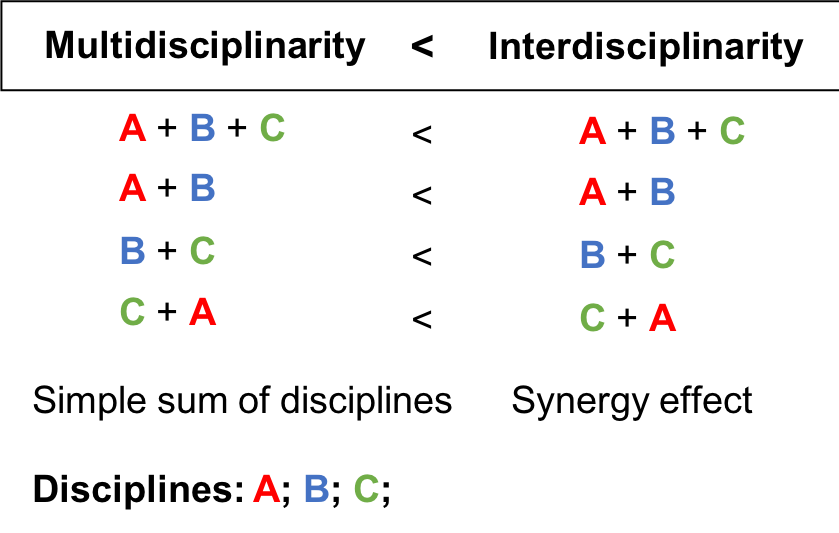
\includegraphics[width=0.6\linewidth]{figures-ext/multidisc} 

}

\caption[Symbolic illustration of sum (multidisciplinarity) versus synergy (interdisciplinarity)]{\textbf{Symbolic illustration of sum
(multidisciplinarity) versus synergy (interdisciplinarity)}, in an
interdisciplinary project sum of thee disciplines A, B, C should have
more value than a simple sum od disciplines: an interdisciplinary
project should have an added value compared to a multidisciplinary one.}\label{fig:multidisc}
\end{figure}







Why not all the labs are interdisciplinary?

\begin{quote}
\emph{Scientists tend to resist interdisciplinary inquiries into their
own territory. In many instances, such parochialism is founded on the
fear that intrusion from other disciplines would compete unfairly for
limited financial resources and thus diminish their own opportunity for
research} ---
\href{http://www.azquotes.com/author/28130-Hannes_Alfven}{Hannes Alfvén}
\end{quote}

Crossing frontiers is not an easy task, and it was quite difficult in
the beginnings of modern interdisciplinarity. Some examples of early
interdisciplinary efforts of 20th century are nicely described by
Ledford et al. \citep{Ledford2015} in \emph{Nature} special issue on
\href{https://www.nature.com/news/interdisciplinarity-1.18295}{Interdisciplinarity}.
It illustrates Theodore Brown in 1980s, while trying to organise a new
interdisciplinary research project and reorganise university space to
engage exchange between students of different faculties, he encounter a
lot of reluctance.

\begin{quote}
\emph{And then there was the stigma. ``Interdisciplinary research is for
people who aren't good enough to make it in their own field,'' an
illustrious physicist chided} \citep{Ledford2015}.
\end{quote}

The story seems to end up with a happy ending of 40-milion US dollars
grant and foundation of Beckman Institute for Advanced Science and
Technology. However, recruiting open-minded director to lead this
unconventional organisation was a struggle. Soon, the organisation
became a model for others and met a great scientific and technological
success.

Even though, since then the idea of interdisciplinary research spread
around the world. Still, not all problem got overcome.

\begin{quote}
\emph{``There's a huge push to call your work interdisciplinary,'' says
David Wood, a bioengineer at the University of Minnesota in Minneapolis.
``But there's still resistance to doing actual interdisciplinary
science''.}
\end{quote}

First, the institutions, universities where research is performed should
equip scientist with a passport to other disciplines, facilitate
exchange, funding the interdisciplinary research, accepting fusion of
disciplines as new ones. Then, a proper communication between
disciplines is necessary. Finally, forming interdisciplinary researches
is extremely challenging as it often requires extra effort from an
apprentice.

\emph{Are all the disciplines idependent units nowadays?}

Can we do molecular biology without technical, mathematical and
computational support? Can we study cognitive science without knowledge
of biology, physics and psychology? Can we advance medecine without
basic research in biology, physiology, electronics?

Bioinformatics and/or computational biology is an interesting case.
Working in this field being between biology, medecine, computer science,
mathematics and statistics, the role of a computational biologist is
sometimes reduced to a service. A biological lab may need a
computational biologist to perform an analysis, restructure the data,
that is needed for the biological discovery. Often, there is not enough
space for research in computational biology itself, where the discovery
does not depend on the original data but on tools and approaches to
complex, data-intensive biological problems. It may happen also the
other way round, when a computational biologist ask a bench researcher
to perform an experiment to prove his theoretical model. In both cases,
the long-term interdisciplinary partnership would probably fail. A wet
and dry researchers should collaborate as equal with important research
advances on both side to assure a long term equilibrium.

\emph{How interdisciplinarity changed over years? Are all disciplines
affected equally?}

From the chart (Fig. \ref{fig:interdisciplinary}) we can see that Social
Studies of Medicine seems to be the most interdisciplinary field. In
general Biology, Health and Biomedical Sciences seem to be more open
into flow of knowledge from other fields than humanities. On the extreme
opposite of health, Clinical Medecine appears to be very conservative
field.

\begin{figure}

{\centering 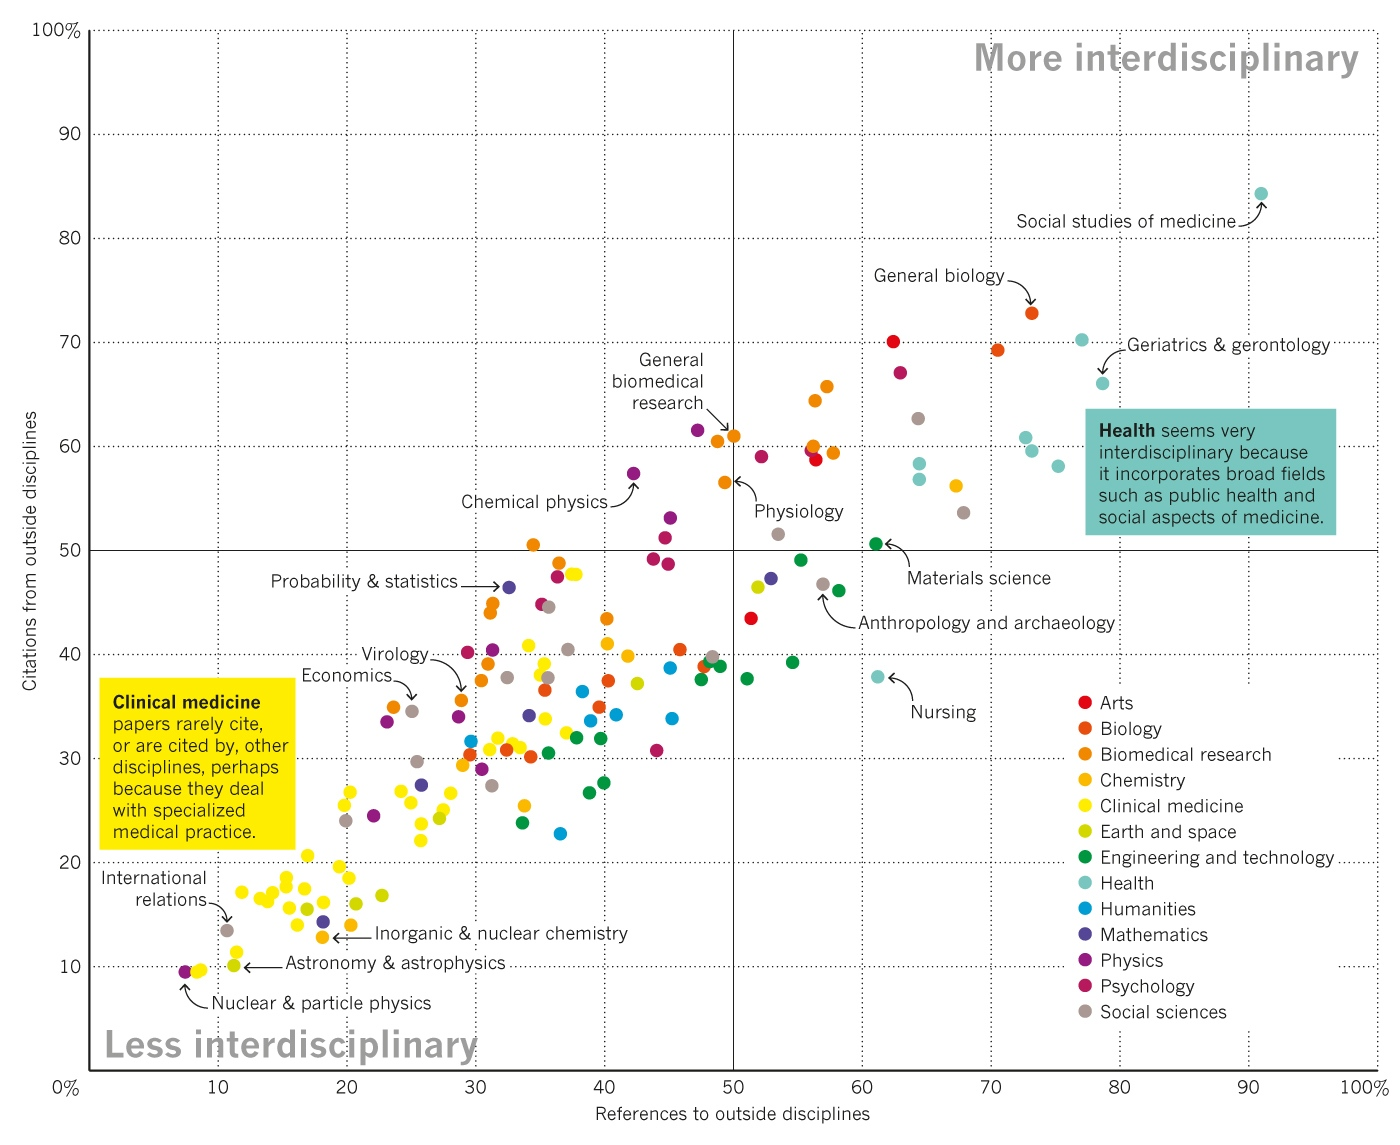
\includegraphics[width=0.9\linewidth]{figures-ext/interdisciplinary} 

}

\caption[Interdisciplnarity of different fields.]{\textbf{Interdisciplnarity of different
fields.} ``From 1950-2014, a field's position is determined by how much
its papers cite outside disciplines (x-axis), and by how much outside
disciplines subsequently cite its papers (y-axis). (Some years, certain
fields have too few references to be plotted.)''. Reprinted by
permission from Springer Nature \citep{VanNoorden2015} © 2015 Nature
America, Inc.~All rights reserved.}\label{fig:interdisciplinary}
\end{figure}









\hypertarget{strengths-weaknesses-opportunities-threats-swot-of-an-interdisciplinary-phd---personal-perspective}{%
\section*{Strengths, Weaknesses Opportunities, Threats (SWOT) of an
interdisciplinary PhD - personal
perspective}\label{strengths-weaknesses-opportunities-threats-swot-of-an-interdisciplinary-phd---personal-perspective}}
\addcontentsline{toc}{section}{Strengths, Weaknesses Opportunities,
Threats (SWOT) of an interdisciplinary PhD - personal perspective}

\begin{quote}
\emph{I'm not good enough to do well something I dislike. In fact, I
find it hard enough to do well something that I like} --- Jim Watson,
Succeeding In Science: Some Rules Of Thumb \citep{Csermely2007}
\end{quote}

Being formed first in double major in biology and mathematics, then
participating in interdisciplinary research projects during my master
studies, I can witness that the learning curve of multiple disciplines
can be steep. It is also often associated with frustration of not going
deep enough in all of disciplines or the feeling of being overwhelmed by
the amount of knowledge.

Coming with expertise of biology and mathematics, I got fascinated by
complex biological systems. One way of study high-dimensional data is to
reduce them into smaller interpretable units. This is what I tempted to
achieve in this thesis in order to enrich our knowledge about tumor
microenvironment and possible contribute to orienting future research on
immunotherapies.

However, being an interdisciplinary researcher was not always a
privilege. \emph{To which category do I belong?} \emph{To whom should I
present my work?} I often asked myself these questions. I also often
encountered lack of understanding where my methodological results were
not bringing enough of \emph{biological insights}. Or the constraints of
my biological application seemed very obscured and complicated for
mathematicians and my work often lacked \emph{important methodological
advances}.

\emph{Does it mean that my work is not accurate, useless?} Probably, for
many, it is not enough. However, I still hope that our findings will be
interesting to some. I enjoy working with data and statistics that serve
an actual purpose. The Tab. \ref{tab:SWOT} summarizes Strengths,
Weaknesses, Opportunities and Threats (SWOT analysis) of an
interdisciplinary projects, in the way I see it.

\rowcolors{2}{gray!6}{white}\begin{table}

\caption[SWOT analysis of Interdisciplinary research]{\label{tab:SWOT}\textbf{SWOT analysis of Interdisciplinary research}.
In SWOT analysis, Strengths, Weakenesses, Opportunities and Threats are
enumerated. Strengths and Wearknesses are internal and Opportunities and
Threats are external factors.}
\centering
\begin{tabular}[t]{|>{\centering\arraybackslash}p{9em}|>{\centering\arraybackslash}p{9em}|>{\centering\arraybackslash}p{9em}|>{\centering\arraybackslash}p{9em}|}
\hiderowcolors
\toprule
\rowcolor{Gray}  \textcolor{white}{\textbf{Strengths (internal, positive)}} & \textcolor{white}{\textbf{Weaknesses (internal, negative)}} & \textcolor{white}{\textbf{Opportunities (external, positive)}} & \textcolor{white}{\textbf{Threats (external, negative)}}\\
\midrule
\showrowcolors
Having a holistic view of the problem & Not seeing details of the problem & Mulitple possibilities to convey research & Spending too much time filling knowledge gap\\
Being supervised by multiple experts & Following multiple, sometimes contradictory,  advice on the same problem & Take advantage of synergistic effect of fields & Inhibiting effect of oppinions from different fields\\
Joining expertises of different fields & Not covering in details all the disciplines & Doing a new discovery & Obtaining too generic results\\
Using new/non standard approach & Experiencing steep learning curve & Raising interest in different expert domains & Not mastering the specific vocabulary of different fields\\
Having better understanding of complex processes & Being in constant need of help of domain experts & Making progress & Not being understood\\
\addlinespace
Higher creativity &  & Creating a new field & Being hard to classify/ fall into a category\\
Having great flexibility &  & Sovling many problems impossible to solve with traditional approach & Being considered as superficial\\
Feeling a thrill of adventure &  &  & \\
Being open &  &  & \\
\bottomrule
\end{tabular}
\end{table}\rowcolors{2}{white}{white}






Besides conducting research that crosses the boundaries of one
discipline, I also could meet and work with inspiring people coping like
me with filling the gap in understanding of an interdisciplinary work,
multiple supervisors and reporting to many institutions. I gained (even
if only superficial) understanding of many topics in mathematics,
statistics, data science, immunology, cancer but also oral and written
presentation skills, time and work management

Is my thesis really interdisciplinary? Does biology profits from
mathematics and mathematics from biology? I will let you judge it.

What impact had biology on the statistical/mathematical modelling ? The
practical problems, systems that go beyond theoretical formulations
challenge the theoretical tools. In my work, I did my best to fuse
theory and practice that should serve a biological application. I can
image the project more complete if the results of my work would inspire
changes in biological experiments, uncover new paths to follow for
experimental biologists or translational researchers.

\hypertarget{the-origins-of-the-phd-topic}{%
\section*{The origins of the PhD
topic}\label{the-origins-of-the-phd-topic}}
\addcontentsline{toc}{section}{The origins of the PhD topic}

\begin{quote}
\emph{The universe will lead me where I need to go. I am like a leaf in
the stream of creation} --- Dirk Gently, Holistic detective
\end{quote}

When finishing my master I was looking for an interdisciplinary subject
where I could deepen my quantitative skills and apply to a real-life
healthcare problem. I came across a project proposed by Andrei Zinovyev
in close collaboration with Vassili Soumelis. I was quite anxious that
my knowledge of cancer immunology would not be sufficient to lead the
project to a success. I recognise that the complexity and heterogeneity
of immune systems are is very complex and dynamic system and many years
of expertise are needed to really grasp the understanding of it. I had a
great chance to work hand in hand with domain experts that would suggest
me the direction I should take in my research.

The project started by causal exploration of different blind source
separation or dimension reduction techniques and their ability to
dissect bulk transcriptomic data into cell type-related units. We also
faced an important problem of lack of gold standard data that would
define efficiency and accuracy of different methods.

I have spent void efforts working on a bulk transcriptomic data
simulation framework, important statistical issues come into our way and
probably another Ph.D would be necessary to solve them. In the meantime,
many tools dissecting tumor bulk transcriptome were published. Serving a
similar purpose, they used different means and assumptions, which left a
space for my project to continue. In my third year, I am finally
publishing a tool that performs the analysis I developed together with
the Sysbio team members, and I can apply it to a corpus of publicly
available data to learn about actual question: the immune system
infiltrating cancers and the context-dependent signatures (see
\protect\hyperlink{deconica}{Chapters 4 \& 5}).

In a parallel project, I worked on exploration of brand new data type:
single cell transcriptomic (RNAseq) in the context of tumor
microenvironment (see \protect\hyperlink{map}{Chapter 6}).

We have also participated in Dream Idea Challenge, a project that aimed
to put closer experimental and theoretical researchers
\citep{Azencott2018}\href{}{Annexe1}.

I have collaborated in numerous projects within and outside my team.
Some of the projects resulted in publications, such as my work on
analysing pDC subsets of X cancer \href{}{Annexe2}. Others are in still
preparation.

Alongside with pursuing the compelling scientific research, I completed
a wide variety of courses. Thanks to this extensive (\textgreater{}300
hours of training over 3 years), I am equipped with soft skills that not
only helped me to shape my thesis project on the go but also, I hope,
will help me to succeed in my future career path.

\hypertarget{organisation-of-the-dissertation}{%
\chapter*{Organisation of the
dissertation}\label{organisation-of-the-dissertation}}
\addcontentsline{toc}{chapter}{Organisation of the dissertation}

\chaptermark{Organisation of the dissertation}

As it is a fruit of an interdisciplinary work, I decided to introduce
the topic from two perspectives: describe the biological and biomedical
dimension of the topic (see \protect\hyperlink{intro}{Chapter 1}), as
well as, the mathematical dimension of the problem of separation of
sources in complex mixtures (see \protect\hyperlink{methods}{Chapter
2}). I hope, it will make the subject of my thesis easy to understand
also for non-biologists or non-mathematicians. In the results part, I
compare reproducibility of blind source separation methods NMF and ICA
(see \protect\hyperlink{sens}{Chapter 4}), I cite our results on the
estimating the Most Reproductible Transciptomic Dimension (MSTD). I also
apply ICA-based deconvolution to Breast cancer transcriptomes to to
prove its reproducibility \protect\hyperlink{LVA}{Chapter 3}. Then I
introduce the DeconICA R package (see
\protect\hyperlink{deconica}{Chapter 5} ) and finally present results of
application of DeconICA and other tools to \textgreater{}100
transcriptomic datasets (see \protect\hyperlink{results}{Chapter 6}). A
second part of results is dedicated to my work on cell type
heterogeneity (see \protect\hyperlink{map}{Chapter 7}). The manuscript
finishes with \protect\hyperlink{conclusions}{Chapter 8} that contains
discussion, conclussions and perspectives. In annexes you can find
publications to which I contributed during my doctorate that are not
strictly linked with the topic of this thesis.

\textbf{INTRODUCTION}

\begin{itemize}
\item
  \protect\hyperlink{intro}{Chapter 1}: introduction to cancer biology
  and immunity, challenges in cancer immunotherapies and cancer immune
  phenotyping as well as data sources most commonly used to face the
  topic.
\item
  \protect\hyperlink{methods}{Chapter 2}: introduction to a problem of
  mixed sources in biological samples, overview of blind source
  separation methods and supervised deconvolution methods, with focus on
  those applied to bulk transcriptome to uncover and quantify immune
  compartments
\end{itemize}

\textbf{RESULTS}

\begin{itemize}
\tightlist
\item
  \href{}{Chapter 3}: Most Reproducible Transcriptome Dimension (MSTD)
\item
  \href{}{Chapter 4}: application of ICA-based deconvolution to six
  breast transcriptomes
\item
  \protect\hyperlink{sens}{Chapter 5}: comparison of reproducibility of
  NMF and ICA methods
\item
  \href{}{Chapter 6}: DeconICA R package
\item
  \href{}{Chapter 7}: application of DeconICA R package and other tools
  to analyse \textgreater{}100 transcriptome datasets of bulk cancer
  transcriptomes
\item
  \protect\hyperlink{map}{Chapter 8}: study of immune cell types
  heterogeneity in tumor microenvironment using innate immune map and
  scRNAseq data
\end{itemize}

\textbf{DISCUSSION}

\begin{itemize}
\tightlist
\item
  \protect\hyperlink{conclusions}{Chapter 9}: discussion, conclussions
  and perspectives
\end{itemize}

\textbf{ANNEXES}

\begin{itemize}
\tightlist
\item
  Other publicatons:

  \begin{itemize}
  \tightlist
  \item
    pDC subsets
  \item
    Idea Dream Challenge
  \end{itemize}
\end{itemize}

\hypertarget{part-introduction}{%
\part{Introduction}\label{part-introduction}}

\hypertarget{intro}{%
\chapter{Immuno-biology of cancer}\label{intro}}

This chapter will first introduce a short history of cancer with a focus
on discoveries linking cancer and its environment. It will also describe
participation of TME in cancer development, progression and response to
treatment. Most important types of data used to study cancer
microenvironment will be discussed. I also introduce a link between
tumor immune-biology and cancer phenotyping for development of
immunotherapies.

\hypertarget{cancer-disease}{%
\section{Cancer disease}\label{cancer-disease}}

According to
\href{http://globocan.iarc.fr/Pages/fact_sheets_cancer.aspx}{GLOBOCAN
study} \citep{GLOBOCAN}, 14.1 million cancer cases was estimated to
happen around the world in 2012. It touched 7.4 million men and 6.7
million women. It is estimated that the cancer cases will increase
almost two-fold to 24 million by 2035.

In France only, in 2012 there were 349426 cases of cancer, of which
leading is Prostate cancer (16,3\%) followed by Breast (14\%) and Lung
(11,5\%).

For a long time studying tumor was focused on tumor cells, their
reprogramming, mutations. Cancer was seen as disease of uncontrolled
cells by the mainstream research. At the same time, the idea of
importance of the impact of other cells and structures on cancer cells
was present but often not believed. Recent success of immunotherapies
moved research focus to tumor cells in their context: tumor
microenvironment. We will describe here what is the composition and role
of the TME in tumor progression, diagnosis and response to treatment.

\hypertarget{hist}{%
\subsection{Historical understanding of cancer}\label{hist}}

Cancer was historically described by a physician Hippocrates (460--370
B.C) \citep{Sudhakar2009}. Even though there exist even earlier evidence
of the disease. Hippocrates stated that the body contained 4 humors
(body fluids) : blood, phlegm, yellow bile and black bile. Any imbalance
of these fluids will result in disease. Particularly the excess of black
bile in an organ was meant to provoke cancer. For years, it was not
known what factors cause cancer and it was easily confounded with other
diseases. In the middle ages in the Renaissance Period it was believed
cancer is a punishment for the sins they committed against their god,
that they deserved it to some extend

Until 18th century it was believed that cancer is contagious and is
spread by parasites.

In the 19th century, tumor cells started to be analysed by pathologists.
They were strike with their ability to proliferate uncontrollably,
ability to spread and destroy the original tissue \citep{NPR2010}.
Around the same time leukocytes from the blood was first described by
Gabriel Andra and William Addison. Just a few years later, in 1845
Bennett and Virchow described blood cells in leukaemia (Fig.
\ref{fig:Virchow-cell}). Virchow is also a father of Chronic irritation
theory (nowadays calledl chronic inflammation) that says that cancer is
caused by local ``irritation'' and, incorrectly, that cancer cells
spread like liquid resulting in metastasis.

\begin{figure}

{\centering 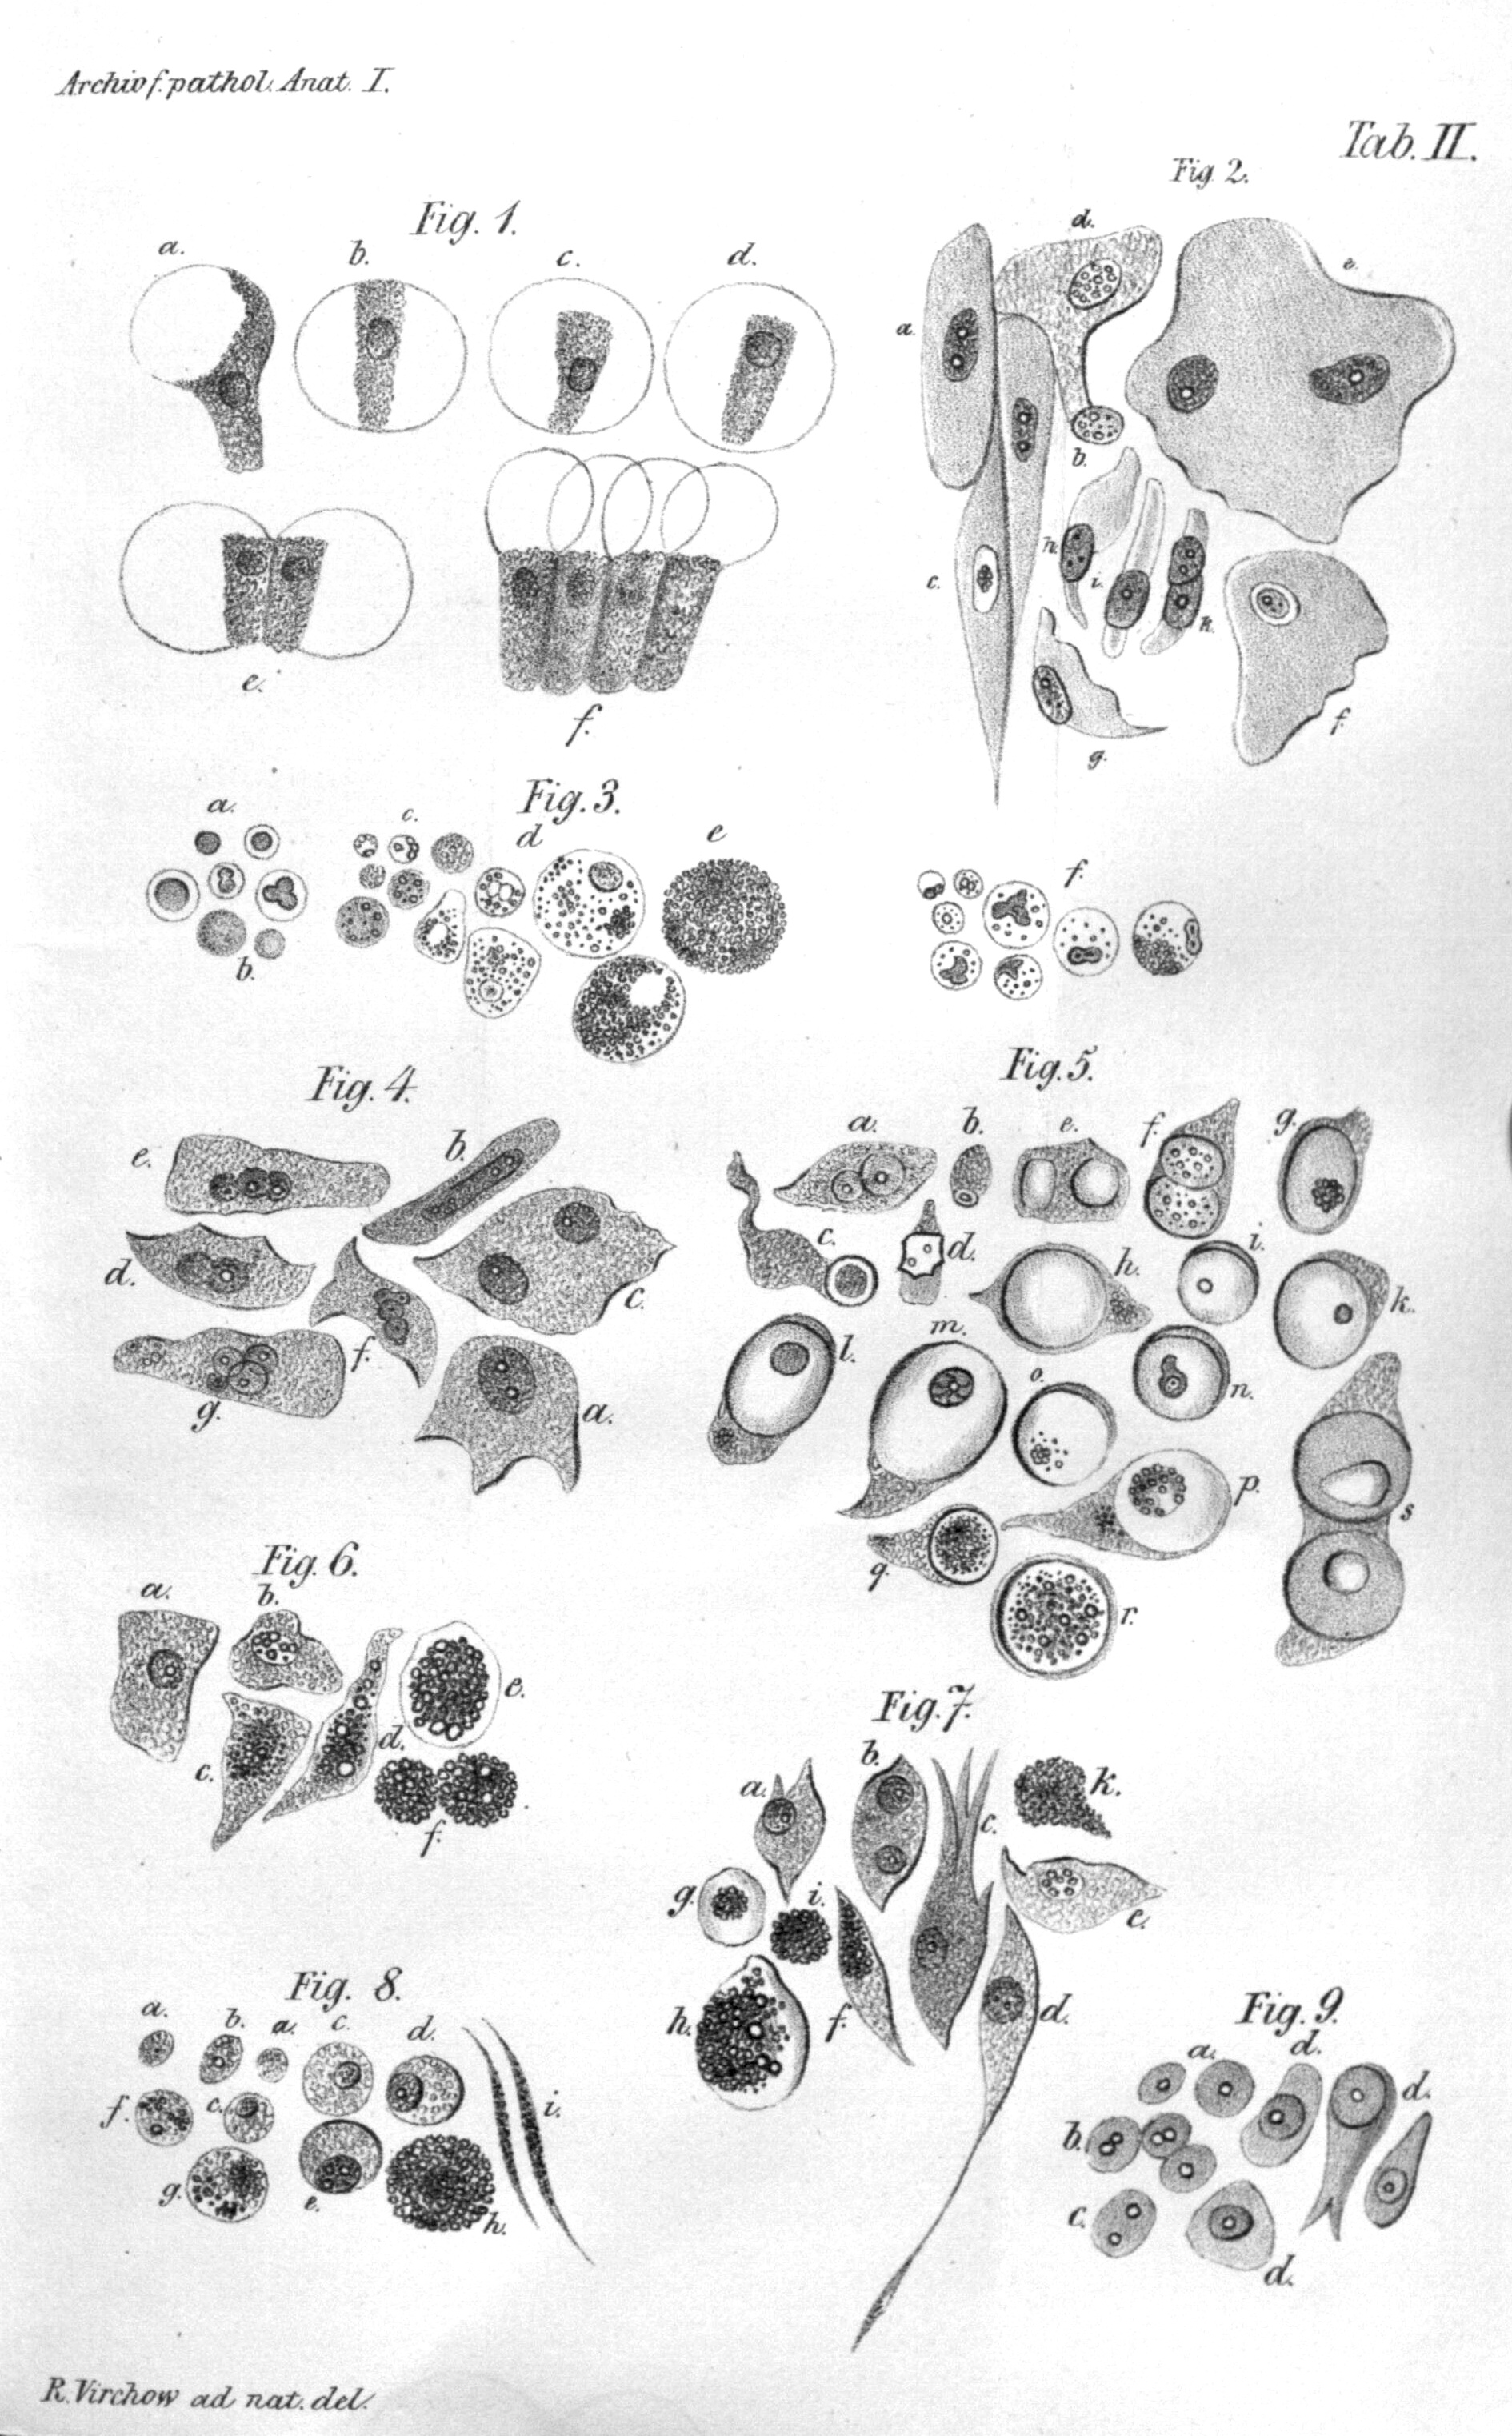
\includegraphics[width=1\linewidth]{figures-ext/01-Virchow-cell} 

}

\caption[Illustration of Virchow's cell theory]{\textbf{Illustration of Virchow's cell
theory}. Virchow depicted different cells transformation due to
irritation. \citep{VirchowRudolf1847}}\label{fig:Virchow-cell}
\end{figure}





In 1889, Stephen Paget introduced \emph{soil and seed} hypothesis of
metastases \citep{Paget1889}. He formulates it as follows

\begin{quote}
\emph{When a plant goes to seed, its seeds are carried in all
directions, but they can only live and grow if they fall on congenial
soil.}
\end{quote}

Which is a parallel to cancer cells disseminated by body fluids, and
they can grow only tissues - ``soil'' that is predisposed to host the
cancer cell - ``the seed''. He focused on the importance of tissue
characteristics that favorise tumor development as opposed to most
researchers of his time that were focusing on the ``seed'' itself.

In the 20th century, molecular causes started to be investigated. It was
discovered that cancer could be caused by environmental factors,
i.e.~chemicals (carcinogens), radiation, viruses and also inherited from
ancestors. Those factors would damage but contrary to a healthy
condition they would not die.

Also in 1909, Paul Ehrlich, called one of fathers of immunology and
Nobel Prize laureate, indicated a link between immune system and tumor
suppression \citep{Ehrlich1909}. One of remarkable first immontherapy
attempts can be attributed to William Coley, that practiced injecting
streptococcus bacteria directly into patients after cancer surgery in
1891, later called ``Colley vaccine''. However, the impact of this
procedure on patients recovery was judged by scientific community as
``unclear''.

In 1968, Melvin Greenblatt and Philippe Shubik showed that tumour
transplants secete a substance stimulating the growth of blood vessels
\citep{Greenblatt1968}, later identified as ``tumour angiogenic factor
(TAF)'' by Judah Folkman in 1971 \citep{Folkman1971}. Folkman also
suggested that TAF can be a target of a therapy itself. This was a
revolutionary idea, at the time, as it did not target the tumor cells
directly acted on thier environment.

During the 1970s, oncogenes and tumor suppressor genes were discovered.
Oncogenes are genes that allow a cell to become cancer cell, while the
tumor suppressor genes would repair DNA or execute cell death of a
damaged cell. A new dimension to cancer studies was added in the 1980s,
epigenetic changes was proven to occur to both oncogenes and tumour
suppressors \citep{Feinberg1983, Greger1989}, which are presently known
as epigenetic markers used for diagnostics and therapeutic targets for
cancer.

In 1982, Aline van Pel and Thierry Boon \citep{VanPel1982} discovered
that a specific immunity to spontanious tumor cells could be induced by
vaccinating mice with mutagenized tumour cells. This araised an
inspiration for many years of immune therapy developement.

In Napoleone Ferrara and colleagues identified gene encoding vascular
endothelial growth factor (VEGF) that was shown to stimulate growth of
enothelial cells proliferation \emph{in vitro} and angiogenesis (blood
vessels formation) \emph{in vivo} \citep{Leung1989}.

In 1999 for the first time, gene-expression was used to study cancer
(leukeamia) by Todd Golub, Donna Slonim and colleagues
\citep{Golub1999}.

Since the end of the 20th century, cancer screens are developed along
with multiple strategies to fight tumor. Most classical ones are based
on the idea of removing tumor cells (surgery), killing tumor cells with
DNA-blocking drugs (chemotherapy), radiation, inhibit cancer growth
(hormonal therapy, adjuvant therapy and immunotherapy). As non of those
methods is fully efficient, often a combination of treatments is
proposed. Nowadays, science is aming in the direction of trageted
therapies and personalized treatment.

The recent success of immunotherapies (discussed in
\protect\hyperlink{immunotherapies}{Immunotherapies section} attracted
the attention the scientific community again to the context in which
tumor cells are found. This context called Tumor Microenvironment, as
well as the communication that happens within it between different
agents, nowadays studied differently with available knowledge of
molecular biology, have become a popular scientific topics of 21st
century (Fig. \ref{fig:pubmedTME}).

\begin{figure}

{\centering 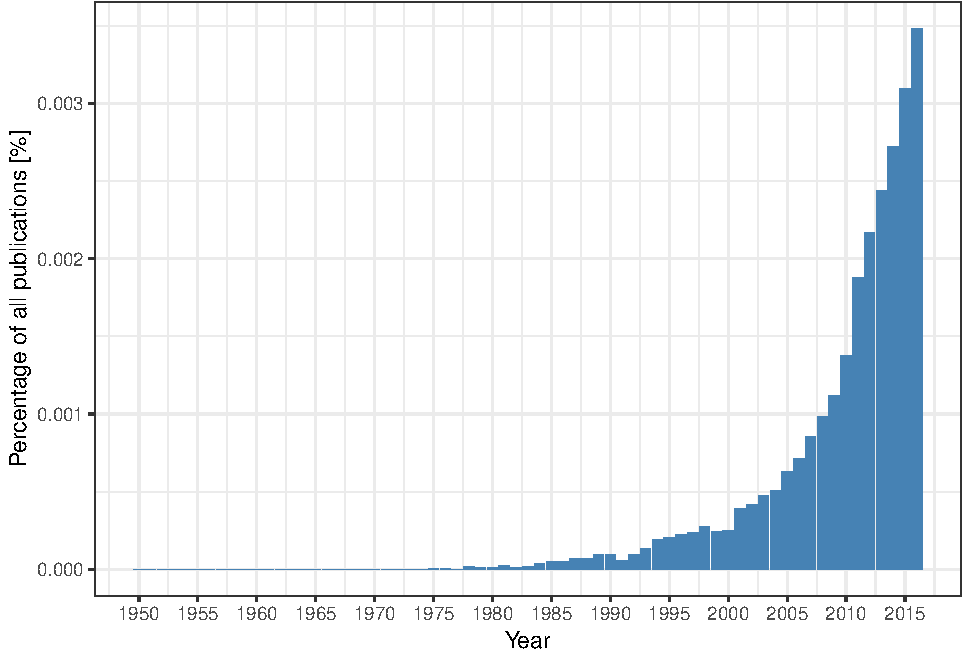
\includegraphics[width=0.7\linewidth]{UCzPhDThesis_files/figure-latex/pubmedTME-1} 

}

\caption[Percentage of publications containg phrase "tumor immunotherapy" is growing]{\textbf{Percentage of publications containg
phrase ``tumor immunotherapy'' is growing}, numbers retreived on
17.01.2018 from \href{http://dan.corlan.net/medline-trend.html}{Medline
Trends} \citep{Corlan2004}}\label{fig:pubmedTME}
\end{figure}






\hypertarget{tumor-microenvironment-as-a-complex-system}{%
\subsection{Tumor Microenvironment as a complex
system}\label{tumor-microenvironment-as-a-complex-system}}

Tumor Microenvironment is a complex tissue that surrounds tumor cells.
It is composed of different compartments (in solid tumors):

\begin{itemize}
\tightlist
\item
  Stroma: blood and lymphatics vessels, epithelial cells, mesenchymal
  stem cells, fibroblasts, adipocytes supported by extracellular matrix
  (EM)
\item
  Immune cells: T cells, B cells, NK cells, Dendritic cells,
  Macorphages, Monocytes etc.
\end{itemize}

Their proportion and specific roles vary significantly with tumor type
and stage. Communication between the environmental cells and the tumor
is critical for tumor development and its impact on patient's response
to treatment. These communication between different compartments is
bidirectional and all the players can influence each other. Depending on
the nature and prevailing direction of those interactions different
destiny is possible for each of the compartments, i.e.~immune cells can
be recruited to protect tumor cells or they can kill them directly. Many
of the signals can be contradictory, many can suppress each other. Then
is it possible to tilt this complex ecosystem into patients' favour? Can
we decipher the most important factors of this molecular knot and
manipulate it?

Next section describes different scenarios of interaction within TME in
order to illustrate the complexity of TME and possible targets for
cancer therapies.

\hypertarget{interactions-between-tme-and-tumor}{%
\subsubsection{Interactions between TME and
Tumor}\label{interactions-between-tme-and-tumor}}

Three scenarios can be considered to describe the relationship between
TME and tumor cells:

\begin{enumerate}
\def\labelenumi{\arabic{enumi}.}
\tightlist
\item
  TME stimulates tumor growth and/or progression and/or impact
  negatively the response to treatment
\item
  TME has no impact on tumor cells and disease development
\item
  TME has a tumor suppressive role and impact positively the response to
  treatment
\end{enumerate}

As can be seen partly in \protect\hyperlink{hist}{Historical
understanding of cancer} these three hypothesis were gaining and loosing
popularity in scientific and medical community over the decades.

\hypertarget{tme-as-a-foe-inflammation}{%
\paragraph{TME as a foe: inflammation}\label{tme-as-a-foe-inflammation}}

In 1863 Rudolf Virchow observed a link between chronic inflammation and
tumorigenesis. According to Virchov theory, genetic damage would be the
``match that lights the fire'' of cancer, and the inflammation or
cytokines produced by immune cells should be the ``fuel that feeds the
flames'' \citep{Balkwill2001}. Therefore lymphocyte infiltration was
confirmed by subsequent studies as a hallmark o cancer. The question one
may ask is why our immune system is not enough to defend the organism
from tumor cells as it does efficiently in a range of bacterial and
viral infections? It is mainly because of the ability of tumor cells to
inhibit immune response through activation of negative regulatory
pathways (so called immune checkpoints).

Many examples can be cited on how TME facilitates tumor development
(Fig. \ref{fig:met-dis}). For instance, in the early stages of
tumorigenesis some macrophage phenotypes support tumor growth and
mobility through TGF-beta signaling. Also, it was shown that NK cells
and myeloid-derived suppressor cells (MDSCs) have an ability to suppress
immune defence i.e.~immunosurveillance by dendritic cells (DCs), T cell
activation and macrophage polarisation and they promote tumor
vascularisation as well. \citep{Talmadge2013, Gabrilovich2012} They
create so-called niches that facilitates tumor colonization. Tregs and
myeloid-derived suppressor cells can negatively impact natural immune
defence and by these means allow growth and invasion of tumor cells
\citep{Taube2017a}. Another cell type, a part of ECM, fibroblast, or
more precisely Cancer Associated Fibroblasts (CAFs) have proven
pro-tumor functions in breast cancer where they enhance metastasis
\citep{Dumont2013}. The blood and lymphatic vessels maintain tumor
growth providing necessary nutritive compound to malignant cells.

\begin{figure}

{\centering \includegraphics[width=1\linewidth]{figures-ext/massive-dissemination} 

}

\caption[The microenvironment supports metastatic dissemination and colonization at secondary sites.]{\textbf{The microenvironment supports metastatic
dissemination and colonization at secondary sites.} Different tumor
sites can communicate through exosomes realized by tumor cells and also
immune and stromal cells such as NK cells, CAFs and DCs. Reprinted by
permission from Springer Nature \citep{Quail2013} © 2013 Nature America,
Inc.~All rights reserved.}\label{fig:met-dis}
\end{figure}








According to \citep{Hanahan2012} immune and stroma cells participate in
almost all of Cancer Hallmarks \citep{Hanahan2000, Hanahan2012}. Most of
the hallmarks of cancer are enabled and sustained to varying degrees
through contributions from repertoires of stromal cell types and
distinctive subcell types.

\hypertarget{tme-seen-as-neutral}{%
\paragraph{TME seen as neutral}\label{tme-seen-as-neutral}}

In front of lack of definitive proof that TME can positively or
negatively impact on tumor development, many scientist, in a long time,
ignored the importance of this factor. Until the early-mid eighties, the
TME research was mostly limited to angiogenesis and immune environment
and most areas that are now driving the field were not represented.

From early 70. until the end of the 90. the most accepted statement was
that genetic alterations in oncogenes and tumor suppressor genes are
both necessary and sufficient to initiate tumorigenesis and drive tumor
progression. Therefore TME was not seen as an important element of the
puzzle.

The cancer geneticists, at the time had a lot of influence on scientific
community diminishing the work of made on TME which were considered as
``uninteresting'' and definitely not ``mainstream''.

After 90s, with discovery of signalling molecules involved in
communication of TME like VEGF general opinion started to change. Also
discoveries made by developmental biology field supported the hypothesis
that microenvironment plays an important role in development which was
later shown for tumorigenesis. Also success of immune vaccines starting
with the tuberculosis vaccine Bacille Calmette-Guérin (BCG) in 1976 and
finishing, at the moment with checkpoint inhibitors did not leave the
scientific community indifferent.

\hypertarget{tme-as-a-friend-immunosurveillance}{%
\paragraph{TME as a friend:
immunosurveillance}\label{tme-as-a-friend-immunosurveillance}}

As mentioned in \protect\hyperlink{hist}{Section 1.1.1} Paget proposed a
hypothesis of ``seed and soil'' where the TME in a certain tissue (the
soil) can either stimulate or suppress the metastasis (the seed).
William Coley tested a possibility to trigger tumorsuppressive effect
via stimulation of the immune system with bacteria. In the 1960s, the
immune surveillance theory hypothesized ``the ability to identify and
destroy nascent tumors as a central asset of the immune system''
\citep{Sebeok1976, Burnet1970}. Thus, the hypothesis that TME can have a
positive role in tumor prognosis is not new.

In modern immuno-oncology, the term \emph{immune-eiditing} was
introduced by \citet{Dunn2002} in 2002, to describe~the relation between
the tumor cells and the immune system. The immunosurveillance through
immune-editing can be summarized in three processes: elimination,
equilibrium, and escape \citep{Dunn2002}.

The elimination is direct killing of cancer cells or growth inhibition
by immune system. The adoptive T cells and NK are actively involved in
tumor killing and stimulate other immune cells. The CD8 + cytotoxic
lymphocytes (CTLs) directly recognize tumor cells. Employing perforin-
and granzyme-dependent mechanisms they can lyze tumor cells. The CD4 + T
cells release factors to induce proliferation of B cells and to promote
their differentiation to antibody (Ab)-secreting plasma cells, activate
macrophages. Macrophages use phagocytosis to eliminate cancer cells
\citep{Vesely2011}.

The tumor-infiltrating lymphocytes (TILs) have been associated with an
overall good prognosis and better survival in different cancer studies.
Also, abundance of CD3 + and CD8 + T cells, NK cells, and
\(\gamma\delta\)T cells correlates with improved outcomes in epithelial
ovarian cancers \citep{Marquez-Medina2012}. Several studies report that
the presence of the abundant immune infiltrate is correlated with good
prognosis or better survival
\citep{Kornstein1983, Baxevanis1994, Naito1998, Pages2005}. Spontaneous
regression of human tumors has been reported in cutaneous melanoma,
retinoblastoma, osteosarcoma, etc. \citep{Aris2012}.

The equilibrium is the phase when cancer and immune cells coexist and
their crosstalk is preventing metastasis.

T cells are the main actor maintaining the equilibrium. Progressively,
the tumor cells become more immunogenic as they are not edited by the
immune system \citep{Bhatia2011}. The state of tumor cells is then
identified as ``dormant'' and active scientific reports investigate the
possible molecular pathways that maintain dormancy or lead to escape
\citep{Teng2008}.

The immune escape is the final process when tumor cells impair the
immune response.

\hypertarget{two-faced-nature-of-immune-cells-context-dependent-functional-plasticity}{%
\subsubsection{Two-faced nature of immune cells: context-dependent
functional
plasticity}\label{two-faced-nature-of-immune-cells-context-dependent-functional-plasticity}}

Modern vision of TME-tumor interactions assumes that tumor can be
directed to several molecular pathways. This direction is decided by
signals that are native of tumor cell and/or coming from the
microenvironment.

Recent studies unveil ambivalent nature of immune cells in TME. While
some as cytotoxic T cells, B cells and macrophages can manage to
eliminate tumor cells. Treg cells role is to regulate expansion and
activation of T and B cells. Depending on cancer type, they can be
either pro- or anti-tumor. For example, as it has been shown for T-regs,
usually associated with bad prognosis, they can be associated with
improved survival (i.e.~in colorectal cancer \citep{Frey2010}). For
innate immunity, there are widely accepted M1 (ani-tumor) and M2
(pro-tumor) extreme macrophages phenotypes in TME \citep{Qian2010}. Most
of the statements seem to be context dependent and not valid universally
across all cancer types. We already mentioned Macrophages phenotypic
plasticity as well as different behaviour of EMC depending on tumor
stage.

From more general point of view, it has been observed that
immunodeficiency can correlate with high cancer incidence. Results of
analysis based on observations of 25,914 female immunosuppressed organ
transplant recipients, the tumor incidence was higher than predicted for
multiple cancers. However, the number of breast cancer cases decreased
which can be really disturbing if we need to decide on the role of
immune defence in tumor progression \citep{Stewart1995}. This indicates
that immune microenvironment can be cancer stimulating or inhibiting
depending on the type of cancer and/or other factors.

\hypertarget{immune-cell-subtypes-in-tme}{%
\subsubsection{Immune cell (sub)types in
TME}\label{immune-cell-subtypes-in-tme}}

We are taught that a cell is the basic structural, functional, and
biological unit of all known living organisms. Human body contains
around \(10^{14}\) which is three order of magnitude more than number of
stars in the Milky Way. This ensemble of cells are traditionally
classified into cell types based on their phenotypical variety.

\begin{quote}
\emph{for their immense number, the variety of cells is much smaller:
only about 200 different cell types are represented in the collection of
about \(10^{14}\) cells that make up our bodies. These cells have
diverse capabilities and, superficially, have remarkably different
shapes\ldots{}.} \citet{Boal2002}
\end{quote}

In the description of TME, I have referred to cell types of immune cells
as well-established entities of immune system. However, the definition
of cell types remains controversial and there is no consensus among
researchers how exactly a cell type should be defined. The notion of the
cell-subtypes is even more vague. The problem does not only concerns
immune cells, most of cell types of our organism, classified initially
according to their morphology, seem to fulfil multiple functions. One
can also relate cell-type problem to species problem where scientist
also debate about where to draw the borders between species. This
problem is widely generalized as ``theory of types'' \citep{Slater2013}
in many disciplines as philosophy, linguistics, mathematics.

In this chapter I will limit the description to immune cell types.

An immune cell can be described nowadays along many axes:

\begin{itemize}
\tightlist
\item
  Phenotype /surface markers
\item
  Stability
\item
  Morphology (expressed proteins)
\item
  Ultrastructure (electron microscopy)
\item
  Molecular data (gene expresson, genotype, epigenome)
\item
  Cell fate
\item
  Cell of origin
\item
  Function
\end{itemize}

Depending how well a cell is different from all other cells along those
axes, it will (or not) be defined as a distinct cell type. However, this
comes with more or less subjective threshold on where the cells become
\emph{significantly different}. This thresholds can be established
computationally or by an expert. Usual practice is a mix of both
methods.

Since the beginning of immunology, there were disagreement between
pre-defined cell types and cell functions.

\begin{quote}
\emph{Cette espèce de leucocytes a une grande ressemblance avec certains
éléments fixes du tissu conjonctif, ainsi qu'avec des cellules
endothéliales et des cellules de la pulpe splénique. On est donc souvent
embarrassé, surtout lorsqu'on trouve ces leucocytes mononucléaires en
dehors des vaisseaux, pour les distinguer des autres espèces de cellules
mentionnées.} --- Elie Metchnikoff, Leçons sur la pathologie comparée de
l'inflammation, 1891
\end{quote}

The definition of cell types and subtypes is widely discussed today with
arrival of single cell technologies that allow a change of paradigm in
cell classifications. Up to now, the top-down approach was mostly used.
Pre-defined set of parameters describing a cell was fixed in order to
select cells and then other parameters were measured. Now, it is
possible to practice bottom-up approach where all (or some) parameters
are measured for a single cell and then, depending on its distance from
other cells, cell types are defined \citep{Satija2014}.

\begin{quote}
\emph{The concept of ``cell type'' is poorly defined and incredibly
useful}\\
--- Allon Klein, Harvard Medical School
\end{quote}

Researchers agree that the concept of cell type is artificial and a
continuum of cell types is closer to the reality. According to Susanne
Rafelski,

\begin{quote}
\emph{A useful way to classify cells might thus be a multiscale and
multi- parameter cell-type space that includes vectors for key
intracellular organizational, dynamic, and functional features as well
as tissue location, gene expression etc.}
\end{quote}

Some, as Allon Klein, propose to introduce a concept of \emph{cell
states} which would better describe a cell depending on its context and
function. However, an emerging challenge would be to connect \emph{cell
states} with historical \emph{cell types.}
\citep{EdiorialCellSystems2017} .

Another aspect of cells, that I am not approaching in this thesis is
time. Cells are shaped by thier environment, intrinsic and extrinsic
events and can change states, functions etc. Can one cell belong to
different cell types depending on its trajectory? How to include the
dynamic aspect of the cells into the classification?

Thus, most scientist agree that used convention of cell types is not
ideal and it is more matter of convenience than biological reality. This
leaves a room to study cells and challenge existing classification.
Describing cell types or cell states in tumor micorenvironment is
extremely interesting as still little is know about the diversity of
cell infiltrated in solid tissues.

\hypertarget{summary}{%
\subsubsection{Summary}\label{summary}}

Cancer is a disease concerning milliards of people with a long history.
Scientific community recognises role of the environment where the tumor
cells find themselves as an important factor influencing tumor
development, prognosis and response to treatment. TME is a complex
environment that constantly interacts with tumor cells, where both tumor
and TME influence and shape each other.

Over the years, many interactions are being discovered and cell types
re-defined and described in their context. However, lots of mechanisms
and interactions of TME remains unknown due to very heterogeneous nature
of this micro environment. This leaves room to more extensive
investigation of TME.

A therapeutic goal are target interactions that would be able to pivot
the essential processes in tumorigenesis or tumor escape in order to put
the cells ``back on track'' and facilitate anti-tumor therapies.

These goals can be meet thanks to improvement of investigation methods,
data quality and abundance. I will discuss the most important data types
used in this project to investigate the TME.

\hypertarget{quantifying-and-qualifying-immune-infiltration-data}{%
\section{Quantifying and qualifying immune infiltration
(data)}\label{quantifying-and-qualifying-immune-infiltration-data}}

Nowadays, more and more biological data is produced. However, this
proliferation of accessible resources is not proportional to generated
insights and wisdom. In this thesis, I aim to generate \emph{Knowledge}
and \emph{Insights} and we hope to generate some \emph{Wisdom} (Fig.
\ref{fig:information-power}). In this section, we will introduce the
foundation of our analysis: different data types that will be further
discussed and explored in chapters that follow.

\begin{figure}

{\centering 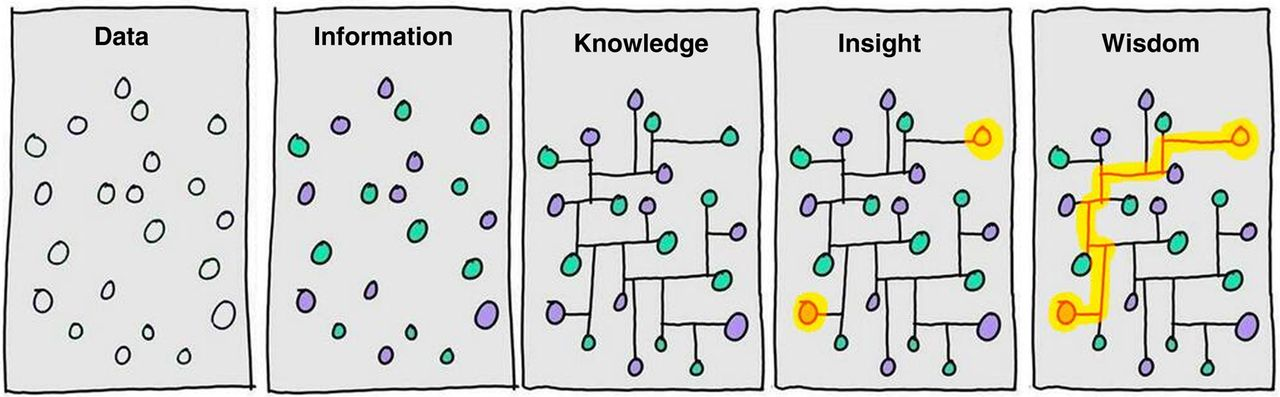
\includegraphics[width=0.8\linewidth]{figures-ext/01-Information_power} 

}

\caption[From Data to Wisdom]{\textbf{From \emph{Data} to
\emph{Wisdom}}. Illustration of different steps that it takes to go from
\emph{Data} to generating \emph{Wisdom}. It highlights that generating
data is not equal to understanding it and additional efforts are needed
to generate value. Image authored by Clifford Stoll and Gary Schubert
published by Portland Press Limited on behalf of the Biochemical Society
and the Royal Society of Biology and distributed under the
\href{https://creativecommons.org/licenses/by/4.0/}{Creative Commons
Attribution License 4.0 (CC-BY)} in \citep{Ponting2017}.}\label{fig:information-power}
\end{figure}











We will introduce most relevant data types that are used to study immune
infiltration of tumors.

\hypertarget{facs}{%
\subsection{Cell sorting}\label{facs}}

\hypertarget{flow-cytometry}{%
\subsubsection{Flow cytometry}\label{flow-cytometry}}

Flow cytometry is a laser-based technology. It uses marker genes: cell
surface proteins to sort cells in different compartments. Nowadays, it
permits quantification of the abundance of up to 17 cell surface
proteins using fluorescently labelled antibodies \citep{Papalexi2017}.
However this techniques is not free from bias, our knowledge about cell
markers is limited and several markers may not be relevant in some
context. Moreover, the scientific community did not clearly agree on the
marker choice even for popular and well studied cell types which
introduced additional heterogeneity when independent studies are
compared. Also the quality of antibodies may influence the results of
the FACs analysis. Besides those limitations FACs remains quite popular
method for analysing cells in complex tissues. It was among first
methods that allowed molecular phenotyping of immune cells, a discovery
of numerous subsets and thier further functional interpretation.

\hypertarget{mass-cytometry}{%
\subsubsection{Mass cytometry}\label{mass-cytometry}}

Mass cytometry (also known as CyTOF allows for the quantification of
cellular protein levels by using isotopes. It allows to quantify up to
40 proteins per cell \citep{Papalexi2017}. It also demands lower
starting number of cells (1000 - 1000000), a realistic number that can
be extracted from patient biopsy \citep{Lyons2017}.

\hypertarget{staining}{%
\subsection{Microscope Staining}\label{staining}}

Using microscope technics, histopathological cuts are analysed. The
number of cells per a unit of area (i.e.~mm\(^2\)) is defined either
manually by human or though diverse image analysis algorithms.

Current pathology practice utilises chromogenic immunohistochemistry
(IHC) \citep{RamosVara2010}. Multiplexed approaches allow to identify
multiple markers in the same histopathology cut. Modern techniques as
imaging mass cytometry using FFPE tissue samples uses fluorescence and
mass cytometry to identify and quantify marker proteins
\citep{Giesen2014}.

The main advantage of aforementioned technics the number of cells that
can be analysed and the information about spatial distribution of the
different cell types. The limiting factor, as for
\protect\hyperlink{facs}{cell sorting methods}, is the number of markers
(\textasciitilde{}10-100) and consequently number of cell types that can
be identified \citep{Schelker2017}.

The \protect\hyperlink{facs}{cell sorting methods} and
\protect\hyperlink{staining}{microscope staining} are usually considered
as a gold standard for multidimensional data techniques. The reason why
they are not applied at large scale is the cost but also quite laborious
and time consuming sample preparation demanding a fresh sample. In
contrast, the \protect\hyperlink{omics}{-omics methods} propose more
scalable way to measure tumor micro environment.

\hypertarget{tissue-microarrays}{%
\subsubsection{Tissue Microarrays}\label{tissue-microarrays}}

Tissue Microarrays aim to automatize ``staining'' techniques. A large
number of small tissue segments can be organised in a single paraffin
block where 100 tissue samples can be easily examined on one slide. A
variety of molecular or microscopic method can be then applied to FFPE
tissue including immunohistochemistry, FISH, and in situ hybridization
\citep{Wilczynski2009}. It is a technique in between traditional imaging
and omic high-throughput.

\hypertarget{omics}{%
\subsection{omics}\label{omics}}

In biological systems information is coded in a form of DNA that do not
vary a lot between different individuals of the same species. In order
to trigger a function in an organism, a part of the DNA is transcribed
to RNA, depending on the intrinsic and extrinsic factors, and after
additional modification messenger RNA (mRNA) is translated into a
protein (i.e.~digestive enzyme) that fulfill a role in the organism. The
mRNA information (also called transcriptome) can be captured with
experimental methods at high throughput (transcriptomics) and provides
an approximation of the state of the studied system (i.e.~a tissue).
There is also information, not coded on the DNA sequence but in a
pattern of chemical species that can regulate the state transition of
DNA information. This additional regulators are called collectively
epigenome and some of them, like methylation, can be also measured at
high-throughput.

\hypertarget{transcriptome}{%
\subsubsection{Transcriptome}\label{transcriptome}}

Transcriptomics measures the number of counts of mRNA molecules using
high-throughput techniques. mRNA is the part of genetic information that
should be translated to proteins. It reflects the activity of ongoing
processes in a cell. In contrast to DNA, mRNA concentration can be
highly variable \citep{Velculescu1997}. This variability can be either
``intrinsic'' that reflect the stochastic process of cell machinery or
``extrinsic'' reflecting impact of factors upstream to mRNA synthesis
\citep{Satija2014}.

Transcriptome can be measured by microarrays or RNA-seq NGS technology.
Microarrays remain cost-efficient and popular technique designed in 90.
There exist two and one color fluorescent probes, both representing
different challenges in experimental design for batch effect removal.
RNA-seq, in contrast, uses sequenced RNA to quantify the expression. As
not only selected genes (probes) are quantified it can be used to study
unknown parts of the genome. RNA-seq is also characterised by lower
background noise than microarrays.

Bulk transcriptome data are quite accessible nowadays. They can be
obtained from either flash-frozen or formalin-fixed, paraffin-embedded
(FFPE) tissue samples, including both surgically resected material and
core needle biopsies \citep{Schelker2017}.

The main flaw of transcriptomic data is that the reproducibility between
different platforms is limited. As a result, direct comparison (direct
merging, statistical difference tests) between two datasets produced by
different platforms is not advised. There are 12 thousands genes that
are matching between four sequencing platforms. Through gene names
conversions a lot of information is lost and bias is introduced.

Different strategies can be adapted to analyse bulk transcriptome.

\citet{Cieslik2017} describes five groups of most popular approaches
that can be applied to study transcriptome (Fig.
\ref{fig:transcriptome-methods}). Despite a diversity of bioinformatic
and statistical tools, the most popular differential approaches, mainly
differential gene expression (DGE) based on difference between two
experimental conditions.

\begin{figure}

{\centering 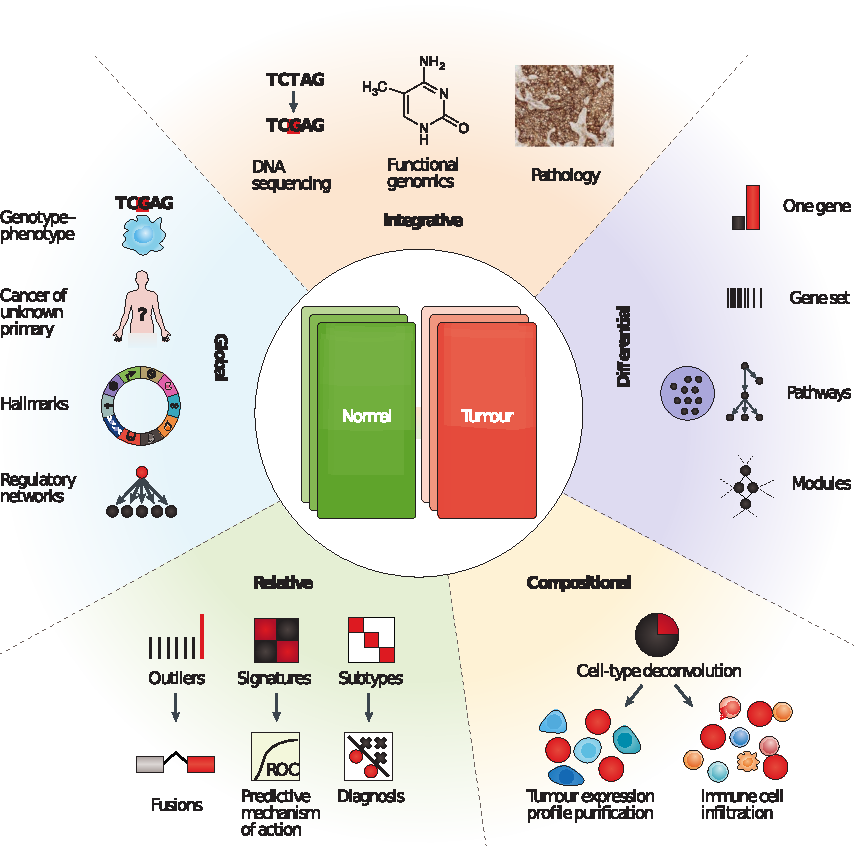
\includegraphics[width=1\linewidth]{figures-ext/transcriptome-methods} 

}

\caption[Five categories of RNA-seq data analysis.]{\textbf{Five categories of RNA-seq
data analysis.} Differential analyses: comparing two (or more)
conditions, Relative analyses: comparing to an internal refernce
(average, base level), Compositional analyses: inferring cell types or
groups of cell types (i.e.~tumor purity), Global analyses: pan-tissue
and pan-cancer analyses and Integrative analyses: compiling
heterogneious data types. Reprinted by permission from Springer Nature
\citep{Cieslik2017} © 2018 Macmillian Publishers Limited, part of
Springler Nature. All rights reserved.}\label{fig:transcriptome-methods}
\end{figure}











RNA-seq data was proven to be a useful indicator for clinical
applications \citep{Mody2015, Oberg2016, Robinson2017}. Its utility for
immune profiling was demonstrated in may studies through a use of
transcriptomic signatures to predict immunotherapy response or survival
\citep{Chen2016}.

In this work transcriptome data analysis fails into multiple categories:
Compositional, Relative and aims to construct a Global-level
conclusions.

\hypertarget{single-cell-rna-seq}{%
\subsubsection{Single cell RNA-seq}\label{single-cell-rna-seq}}

Described above methods of process DNA from hundreds of thousands of
cells simultaneously and report averaged gene expression of all cells.
In contrast, scRNA-seq technology allows getting results for each cell
individually. This is tremendous step forward enhancement of our
understanding of cell heterogeneity and opens new avenues of research
questions.

Continuous discovery of new immune subtypes has proven that cell surface
markers that are used for phenotyping by techniques like
\protect\hyperlink{facs}{FACS} and
\protect\hyperlink{staining}{immunohistochelistry} cannot capture the
full complexity. ScRNA-seq methods allow to cluster known cell types in
subpopulations based on their genetic features. ScRNA-seq is also able
to capture particularly rare cell types as it requires much less of RNA
material (1 ng isolated from 100-1000 cells) compared to `bulk' RNA-seq
( \textasciitilde{} 1 μg of total mRNA transcripts ). It also allows to
study cells at high resolution capturing the phenotypes in much more
refined scale than previously \citep{Papalexi2017}.

This new data type also brings into the field new challenges related to
data processing due to the volume, distribution, noise, and biases.
Experts highlight as the most ``batch effect'', ``noise'' and ``dropout
effect'' \citep{Perkel2017}. So far, there are no official standards
that can be applied which makes data comparison and post-processing even
more challenging. Up to date, there are around 70 reported tools and
resources for single cell data processing \citep{Davis2016} . A limited
number of single-cell datasets of tumors are made publicly available and
more are to come.

One can ask why then developing computational deconvolution of bulk
transcriptome if we can learn relevant information from single-cell
data. Firstly, that single cell data do not provide a straightforward
answer to the estimation of cell proportions. The coverage is not full
and sequenced single cells are not fully representative of the true
population. For instance, neutrophiles are not found in scRNA-seq data
because of they are ``difficult to isolate, highly labile \emph{ex vivo}
and therefore difficult to preserve with current single-cell methods''
\citep{Schelker2017}. In addition, a number of patients included in
published studies of range \textless{}100 cannot be compared to thousand
people cohorts sequenced with bulk transcriptome methods. This is mostly
because single cell experiments are challenging to perform, especially
in clinical setting as fresh samples are needed \citep{Schelker2017}.
Today, single cell technology brings very interesting ``zoom in''
perspective, but it would be incautious to make fundings from a
restricted group of individuals universal to the whole population. Major
brake to the use of single cell technology more broadly might be as well
the price that is nearly 10x higher for single cell sample compared to
bulk \citep{Cedar2018}.

In this work, we are using single cell data in two ways. Firstly, in
\protect\hyperlink{results}{Chapter 5} we compare immune cell profiles
defined by scRNA-seq, blood and blind deconvolution (problem introduced
in \protect\hyperlink{immune-signatures}{Immune signatures section}).
Secondly, in \protect\hyperlink{map}{Chapter 6} we use single call data
of Metastatic melanoma generated by \citet{Tirosh2016} to demonstrate
heterogeneity of subpopulations of Macrophages and NK cells.

\hypertarget{epi}{%
\subsubsection{Epigenome}\label{epi}}

An epigenome can be defined as a record of the chemical changes to the
\textbf{DNA and histone proteins} of an organism. Changes to the
epigenome can provoke changes to the structure of chromatin and changes
to the function of the genome \citep{Bernstein2007}. Epigenome data
usually contains information about methylation \textbf{CpG island
changes}. In cancer, global genomic hypomethylation, CpG island promoter
hypermethylation of tumor suppressor genes, an altered histone code for
critical genes, a global loss of monoacetylated and trimethylated
histone H4 were observed. Methylome profiles can be also use as
molecular signature of disease and potential diagnostic or predictive
biomarker \citep{Jeschke2017}.

\hypertarget{copy-number-variation-cnv-and-copy-number-aberration-cna}{%
\subsubsection{Copy number variation (CNV) and Copy number aberration
(CNA)}\label{copy-number-variation-cnv-and-copy-number-aberration-cna}}

The differences between human genome comes in majority from \textbf{Copy
Number Variation }\citep{McCarroll2007}. CNV regions constitute
~4.8--9.7\%~ of the whole human genome \citep{Zarrei2015}. They can be
reflected in structural variation that are duplication or a deletion of
DNA bases. CNV can affects a lot of base pairs of DNA code (deletion of
more than 100 genes) and result in a phenotype change.

In addition, there can be distinguished, \textbf{Copy number
alterations/aberrations (CNAs)}~that are changes in copy number that
have arisen in~\textbf{somatic}~tissue (for example, just in a tumor),
in contrast to~CNV that~originated from changes in copy number
in~\textbf{germline}~cells (and are thus in all cells of the organism)
\citep{McCarroll2007}. CNV and CNA profiles can be associated with
diseases or cancer subtypes.

There exist disease-related exome panels that focus on regions with high
copy variation or the full exome can be sequenced using whole-exome
sequencing (WES) \citep{Yamamoto2016}.

\hypertarget{spatial-transcriptomics}{%
\subsubsection{Spatial transcriptomics}\label{spatial-transcriptomics}}

\begin{quote}
Spatial transcriptomics provides quantitative gene expression data and
visualization of the distribution of mRNAs within tissue sections and
enables novel types of bioinformatics analyses, valuable in research and
diagnostics \citep{Stahl2016}
\end{quote}

It combines RNA-seq technology with spatial labelling which allows to
have a bulk gene expression of 10-20 cells with given space coordinates
within the sample. It allows to localize regions of highest gene
expression and perform \emph{Spatially Variable Genes}
(\citet{Svensson2018}). Some attempts were already made to combine
Spatial Transcriptomics and scRNA-seq \citep{Moncada2018}. It remains an
early-stage technique and so far it is not widely used but it might be a
future of omics to add a spatial information as it can be essential for
many research problems.

\hypertarget{immunotherapies}{%
\section{From cancer phenotyping to immune
therapies}\label{immunotherapies}}

This section outlines different methods of cancer immune phenotyping and
progress in cancer therapies with a focus on immune therapies. It will
link the ongoing research on TME with therapeutical potential.

\hypertarget{cancer-immune-phenotypes}{%
\subsection{Cancer immune phenotypes}\label{cancer-immune-phenotypes}}

Since 20s century physicians decided on common nomenclature that
classify tumors into distinct groups that are relatively homogenous or
that share common characteristic important for treatment and prognosis.
Tumor typing should help to better predict prognosis, to adapt a therapy
to the clinical situation, to enable therapeutic studies which are
essential in proving any therapeutic progress.

Most of the classifications are based on clinical data. Most common
factors taken into account are: the degree of local invasion, the degree
of remote invasion, histological types of cancer with specific grading
for each type of cancer, possibly various tumour markers, general status
of the patient.

However, cancers with similar morphological and histopathological
features reveal very distinct patterns of progression and response to
therapy \citep{Galon2014}. In the era of gene sequencing, gene and
protein expression as well as epigenome can provide an important
complementary information. Therefore gene markers or proteomic
abnormalities can integrated into classification panel. One popular
example is a gene signature \emph{PAM50} \citep{Parker2009} used for
prediction of patients' prognosis in breast cancer, patented as a tumor
profiling test.

Since the increase of importance of the immunotherapies, researches
proposed several ways to classify tumors based on their
microenvironment. Given different parameters describing TME, cancers can
be sorted into groups that show similar characteristics. We will discuss
most common frameworks that allow to phenotype cancers based on the TME.

The localisation of the immune cells can be an indicator of the state
and response to the therapy \citep{Bindea2013}.

The most standard approach is to convey an analysis of histopathological
cuts to asses the number of infiltrating lymphocytes (TILs). Two typical
patterns are usually identified: ``hot'' - immune inflamed and ``cold''
- no active immune response \citep{Berghoff2018}.

\citet{Chen2017} describe classification into inflamed and non-inflamed
tumors, where non-inlamed phenotypes: can be further split into the
immune-desert phenotype and the immune-excluded phenotype (Fig.
\ref{fig:immune-phenotypes}). The inflamed phenotype is characterised by
rich presence of immune cells : T cells, myeloid cells, monocytes in
tumor margin. Along with the immune cels, due to their communication, a
high expression of cytokines is characteristic for this phenotype.
According to \citet{Chen2017}, this is a mark that an anti-tumor
response was arrested by tumor. The inflamed phenotype has shown to be
most responsive to immunotherapies. In the immune-excluded phenotype,
the immune cells are present as well but located in the stroma
\citep{Herbst2014}, sometimes penetrating inside tumor. However, when
exposed to check point immuotherapy, T cells does not gain the ability
to infiltrate the tumor, therefore the treatment is inefficient. The
immune-desert main features is little or no presence of immune cells,
especially T cells. Surprisingly, this tumors have been to proven to
rarely respond to the checkpoint therapy \citep{Herbst2014}. In
non-inflamed tumours cytokines associated with immune suppression or
tolerance are expressed.

\begin{figure}

{\centering 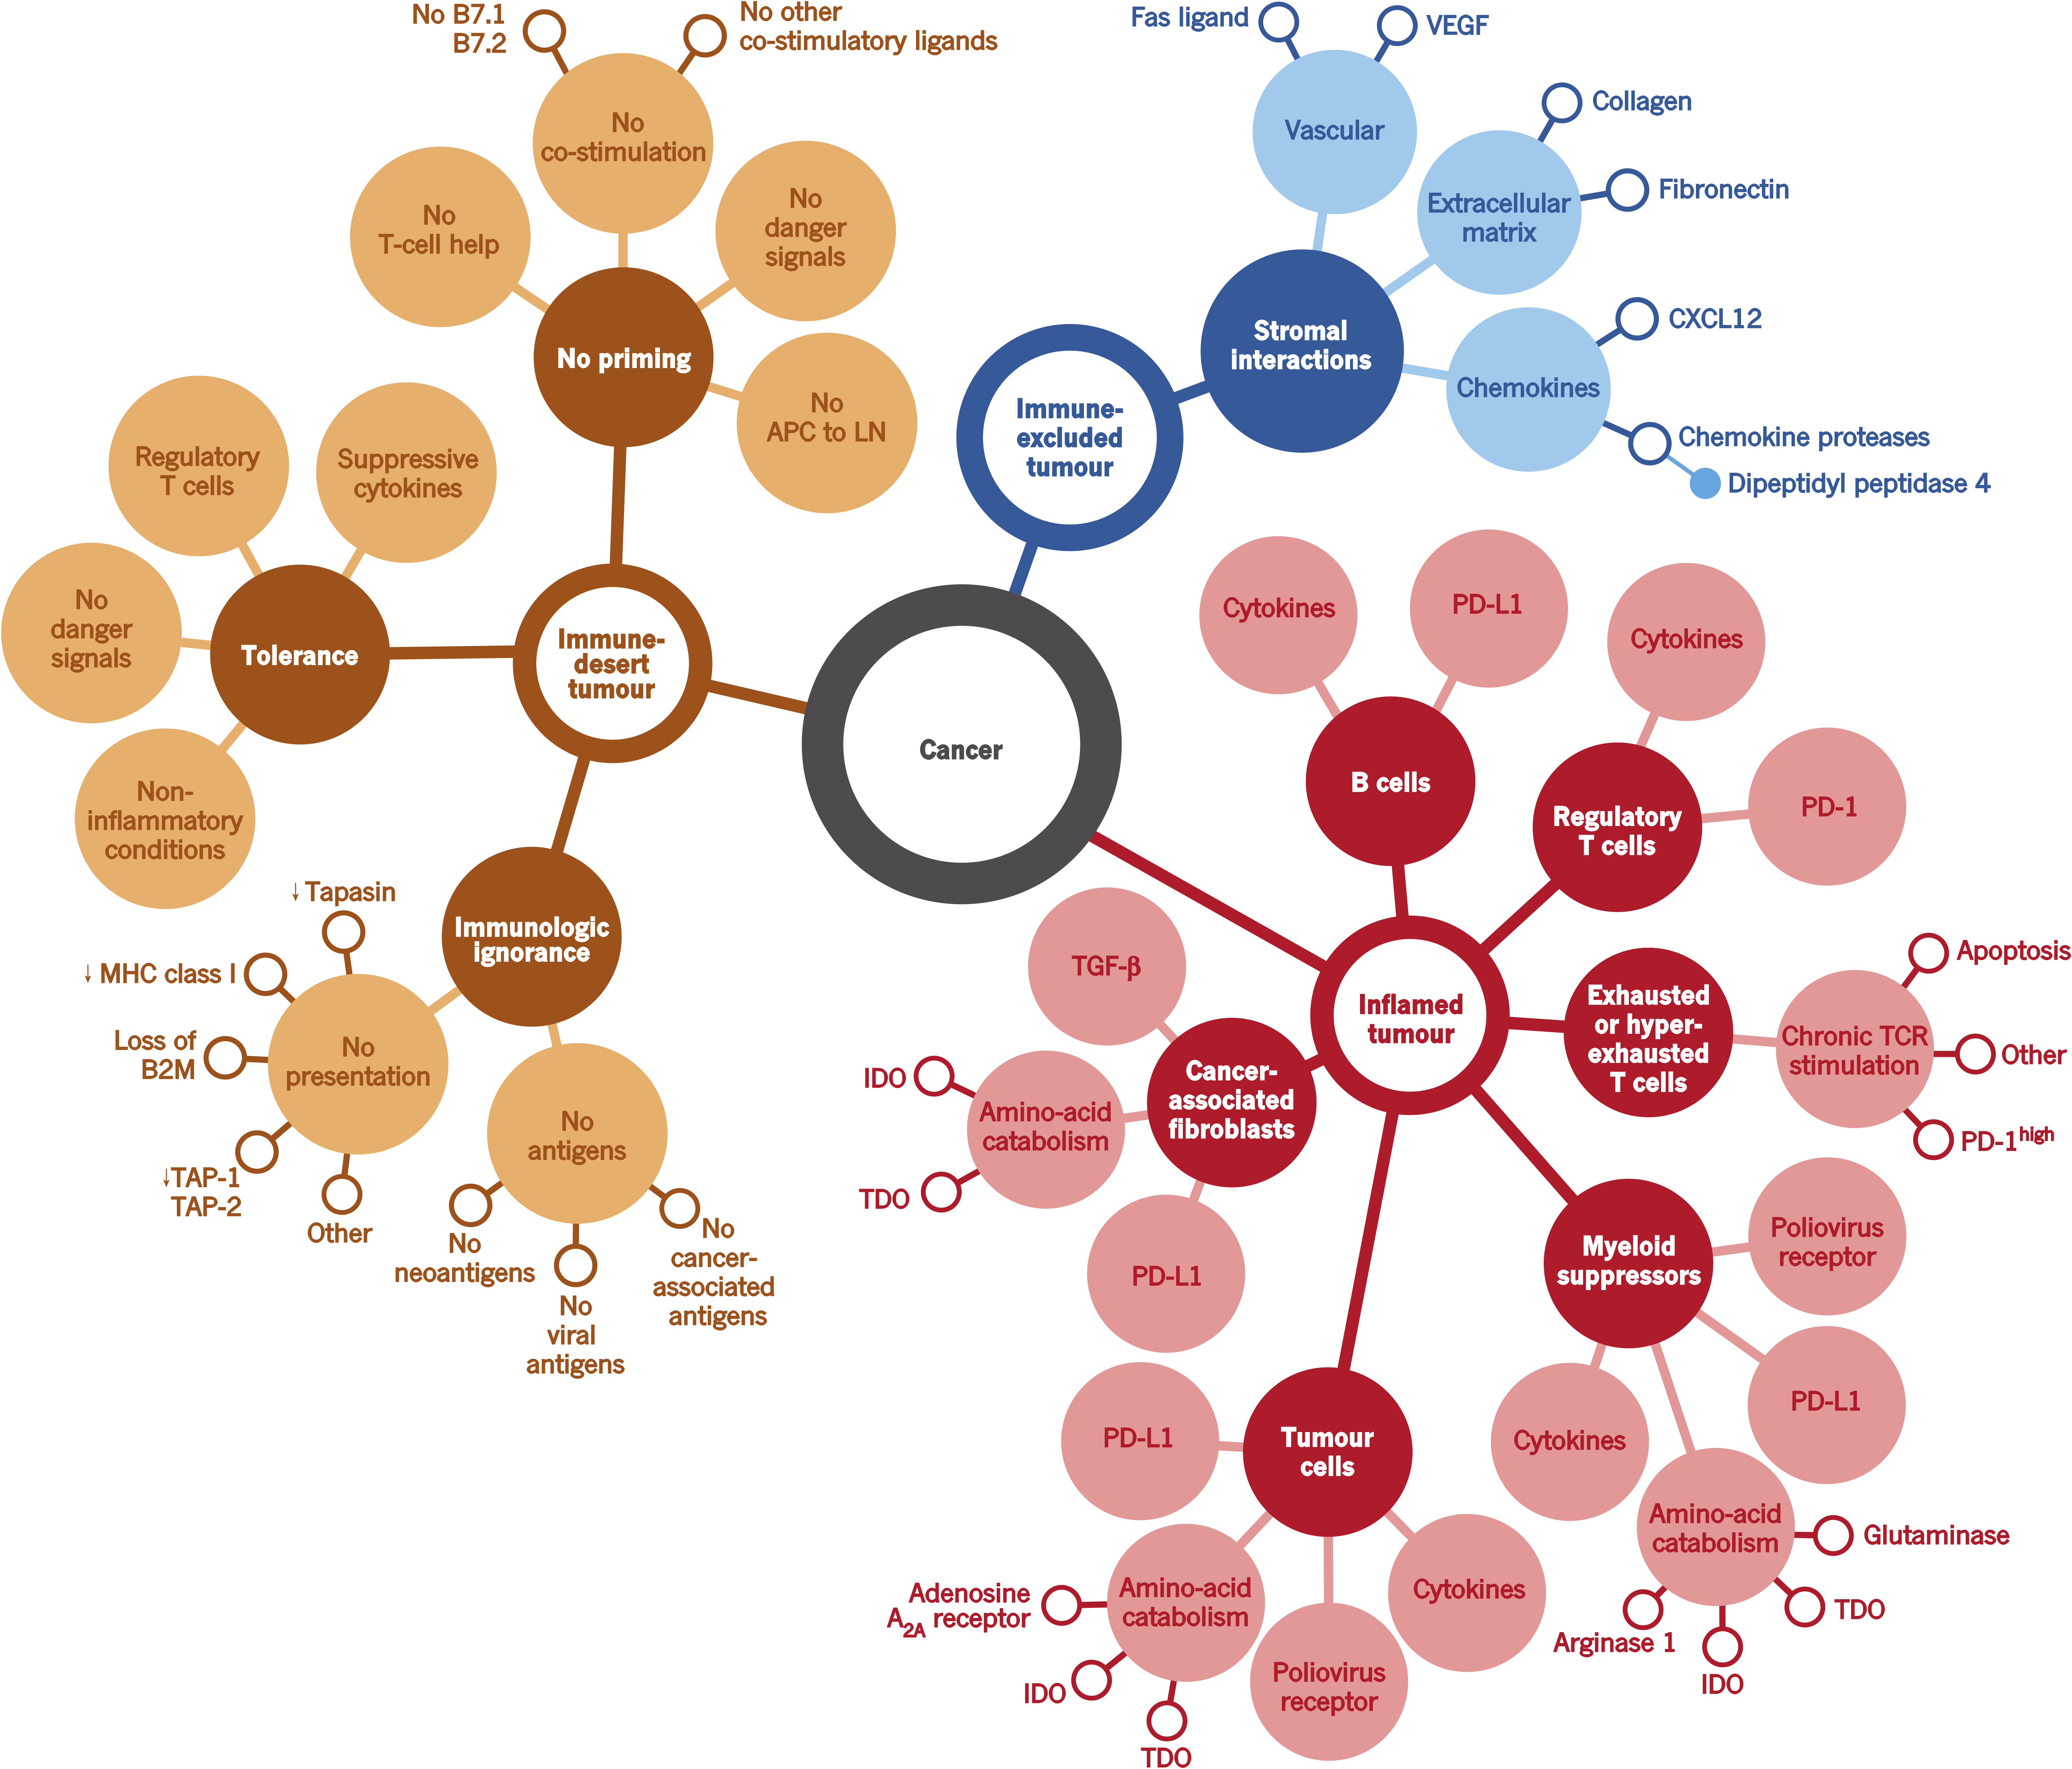
\includegraphics[width=1\linewidth]{figures-ext/immune-phenotypes} 

}

\caption[Cancer-immune phenotypes: the immune-desert phenotype, the immune-excluded phenotype and the inflamed phenotype.]{\textbf{Cancer-immune phenotypes: the
immune-desert phenotype (brown), the immune-excluded phenotype (blue)
and the inflamed phenotype (red).} The immune-desert phenotype is
characterised by paucity of immune cells and cytokines. In the
immune-excluded phenotypes the T cells are often present but trapped in
stroma, enabled to migrate to the tumor site. The immune-inflamed
phenotype is rich in immune cells and the most responsive to the immune
check point therapies. Reprinted by permission from Springer Nature
\citep{Chen2017} © 2017 Macmillian Publishers Limited, part of Springler
Nature. All rights reserved.}\label{fig:immune-phenotypes}
\end{figure}












A presence of immune phenotypes was confirmed by for example by
\citet{Becht2016} in colorectal cancer, where after deconvolution of
bulk tumor profiles, pattern of immune and stroma cells abundance was
matching four cancer subtypes. The good prognosis was related to
cytotoxic response and bad prognosis to lymphocytes and cells of
monocytic origin.

According to \citet{Gajewski2006}, the immunogenicity of the tumors can
be explained by tumor-intrinsic factors and tumor-extrinsic factors.
Tumor-intrinsic factors are: the neoantigen load and frequency, the
mutational load, the expression of immunoinhibitors and
immunostimulators (e.i. PD-L1), and alteration of HLA class I molecules.
Tumor-extrinsic factors include chemokines regulating T cell
trafficking, infiltration of effector TILs and immunosuppressive TILs,
and soluble immunomodulatory factors (cytokines).

\hypertarget{scoring-the-immune-infiltration}{%
\subsection{Scoring the immune
infiltration}\label{scoring-the-immune-infiltration}}

Experimental techniques and computational tools enabled us to
characterize and classify TME with multi-omics data. Here I present a
short list of most influencing and complete analysis aiming to redefine
tumor phenotypes based on the immune infiltration, with a focus on
computational techniques.

\hypertarget{immunoscore}{%
\subsubsection{Immunoscore}\label{immunoscore}}

One of the most recognised scoring method, based on fluorescent images
is authored by Jerôme Galon lab in Paris and names
\href{http://www.haliodx.com/clinical-research-services/immunoscorer/}{Immunoscore}.
The Immunoscore ranges from 0 to 4 and it is based on the density of
lymphocyte populations CD3/CD45RO, CD3/CD8, or CD8/ CD45RO. It also
takes into account the spacial position of the cells: the tumor core and
margins \citep{Galon2012}. It was successfully applied to colorectal
cancer to predict patients' survival \citep{Anitei2014} . Since it
resulted in numerous application to many cancer types. Immunoscore has
been recently validated in big cohort international independent study
(14 centres in 13 countries) as a relevant prognostic score of time to
recurrence, defined as time from surgery to disease recurrence
\citep{Pages2018}.

The immunoscore is an interesting indicator, especially in the scope of
clinical applications, although it does not tell us a lot about
underlying biology. It is also limited to a few cell types while it may
be that in some cancer types or patients, the system requires more
detailed or rich analysis of larger panel of cells.

\hypertarget{spatiotemporal-dynamics-of-intratumoral-immune-cells-of-colorectal-cancer}{%
\subsubsection{Spatiotemporal dynamics of Intratumoral Immune Cells of
Colorectal
Cancer}\label{spatiotemporal-dynamics-of-intratumoral-immune-cells-of-colorectal-cancer}}

\citet{Bindea2013} published very complete, and supported with strong
experimental evidence, immune landscape of colorectal cancer. Authors
introduced \emph{the immunome compendium} containing 577 cell-type
specific genes, derived from analysis of big corpus of publicly
available data. They used it to analyse CRC large transcriptomic data
(105 patients). Using qPCR (more sensitive technique than microarray)
expression of 81 ``representative'' genes from the compendium was
investigated in 153 CRC patients. This study validated correlation of
markers of the same type and also revealed correlation of different
cell-type markers (i.e.~Tcells and NK or Th and macrophages). The data
matrix was grouped into 3 clusters which were corresponding to 1) tumor
2) adaptive 3) innate imune repsonses. In addition spatial positioning
of markers was visualized thanks to Tissue Microarray technology in
samples from 107 CRC patients distinguishing marker densities in tumor
center and tumor margin areas. This was followed by in deep study of
chemokines expression and genomic alterations. In addition, authors
validated potential prognostic biomarkers in murine orthotopic CRC
models.

In summary, using marker genes measured and visualized with different
data types of CRC, a high inter-patient heterogeneity was observed. It
was confirmed that the immune landscape evolves over time (tumor
stages). Adaptive immunity cells were associated with core of the tumor
and the innate ones with the tumor margin. A mechanism involving CXCL13,
Tfh cells, B cells and IL-21 was identified as associated with good
prognosis.

\hypertarget{immunophenoscore}{%
\subsubsection{Immunophenoscore}\label{immunophenoscore}}

Different approaches, sub-typing oriented, are based essentially on gene
expression patterns. Most commonly, machine learning supervised
algorithms are trained to match known phenotype (established with
microscopy or with clinical features) to genetic patterns or an
unsupervised clustering is used to discover new classification.

An example of well-formulated classification framework is
Immunophenoscore \citep{Charoentong2017}, based on publication of
\citet{Angelova2015}, where methylome, transcriptome and mutation of
TCGA CRC dataset (n = 598) was used to describe \emph{immunophenotypes}.
Later on, it was reduced to gene expression indicator and summarised in
a form of a score. This scoring scheme is based on the data of 20 solid
tumors, using expression of marker genes selected by a machine learning
algorithm (random forest) for best prediction in each cancer. These
indicators can be grouped into four categories:

\begin{itemize}
\tightlist
\item
  MHC molecules (MHC)
\item
  Immunomodulators (CP)
\item
  Effector cells (EC)
\item
  Suppressor cells (SC)
\end{itemize}

The immunophenscore (IPS) is calculated on a 0-10 scale based on the
expression of genes in each category. Stimulatory factors (cell types)
impact the score positively and inhibitory factors (cell types)
negatively. Z-scores ≥ 3 were designated as IPS10 and z-scores ≤ 0 are
designated as IPS0. A similar conceptual framework called \emph{cancer
immunogram} was proposed by \citet{Blank2016} included seven parameters:
tumor foreignness (Mutational load), general immune status (Lymphocyte
count), immune cell infiltration (Intratumoral T cells), absence of
checkpoints (PD-L1), absence of soluble inhibitors (IL--6, CRP), absence
of inhibitory tumor metabolism (LDH, glucose utilisation), tumor
sensitivity to immune effectors (MHC expression, IFN-γ sensitivity).
\citet{Charoentong2017} claim that the immunophenoscore can predict
response to CTLA-4 and anti-PD-1.

Nonetheless, the details of the use of \emph{cancer immunogram} in
practice remain unclear and result could be sensitive to patients' and
data heterogeneity as no standardisation was proposed. It should be also
validated in a systematic independent study.

\hypertarget{the-immune-landscape-of-cancer}{%
\subsubsection{The immune landscape of
cancer}\label{the-immune-landscape-of-cancer}}

\rowcolors{2}{gray!6}{white}\begin{table}

\caption[Six immunological subtypes of cancer]{\label{tab:C6}\textbf{Six immunological subtypes of cancer}. General
characteristic of subtypes generated by \citet{Thorsson2018} as
described in the original publication.}
\centering
\resizebox{\linewidth}{!}{
\begin{tabular}[t]{|>{}c|>{}c|>{}c|>{}c|>{}c|>{}c|>{}c|}
\hiderowcolors
\toprule
\rowcolor{Gray}  \textcolor{white}{\textbf{Cluster}} & \textcolor{white}{\textbf{Features}} & \textcolor{white}{\textbf{Macrophage..lymphocyte}} & \textcolor{white}{\textbf{Th1.Th2}} & \textcolor{white}{\textbf{Proliferation}} & \textcolor{white}{\textbf{Intratumoral.heterogeneity}} & \textcolor{white}{\textbf{Other}}\\
\midrule
\showrowcolors
C1 & Wound healing & Balanced & Low & High & High & \\
C2 & IFN-$\gamma$ dominant & Lowest & Lowest & High & Highest & Highest M1 and CD8 T cells\\
C3 & Inflammatory & Balanced & High & Low & Lowest & Highest Th17\\
C4 & Lymphocyte depleted & High & Minimal Th & Moderate & Moderate & \\
C5 & Immunologically quiet & Highest & Minimal Th & Low & Low & Highest M2\\
C6 & TGF-$\beta$ dominant & High & Balanced & Moderate & Moderate & Highest TGF-β signature\\
\bottomrule
\end{tabular}}
\end{table}\rowcolors{2}{white}{white}

\citet{Thorsson2018} performed a multi-omic analysis of TCGA datasets
that allowed them to define 6 subtypes that are valid across cancer
types (see Tab. \ref{tab:C6} ).





Authors selected eight indicators to define these six phenotypes:

\begin{enumerate}
\def\labelenumi{\arabic{enumi}.}
\tightlist
\item
  differences in macrophage or lymphocyte signatures
\item
  Th1:Th2 cell ratio
\item
  extent of intratumoral heterogeneity
\item
  aneuploidy
\item
  extent of neoantigen load
\item
  overall cell proliferation
\item
  expression of immunomodulatory genes
\item
  prognosis
\end{enumerate}

These indicators were selected among many other indicators though
machine learning (elastic net regression) for the best predictive power
of survival.

All the data and computed parameters can be accessed at
\href{https://isb-cgc.shinyapps.io/shiny-iatlas/}{CRI iAtlas Portal}.
Among the six phenotypes C3 (Inflammatory) has the best associated
prognosis while C1 (wound healing) and C2 (IFN-\(\gamma\) dominant),
much less favourable outcome. This again illustrates the ambivalent
nature of the immune system as the best and the worst prognosis are
associated with immunologically active tumors. C4 (lymphocyte depleted)
and C6 (TGF-\(\beta\) dominant) subtypes had the worst prognosis. The
content of immune cells was determined using different tools and data
types (expression, DNA methylation, images etc.) We can learn a lot from
the study, however, it seems difficult to integrate the methods to an
ordinary practice because different data levels are necessary for the
same samples to compute all the indicators.

\hypertarget{a-pan-cancer-landscape-of-immune-cancer-interactions-in-solid-tumors}{%
\subsubsection{A pan-cancer landscape of immune-cancer interactions in
solid
tumors}\label{a-pan-cancer-landscape-of-immune-cancer-interactions-in-solid-tumors}}

A different classification was proposed by \citet{Tamborero2018}, also
using TCGA data. They distinguished 17 immune infiltration patters based
on the immune cell proportions and 6 different clusters based on
cytotoxicity measure across all cancer types (named immune-phenotypes)
that were finally summarized in three groups: cytotoxic immune
infiltrate, infiltrate with more immune-suppressive component and poor
immune infiltrate. According to the analysis, one of the most important
factors is cytotoxicity. Tumors with high cytotoxicity were
characterized by low clonal heterogeneity, with gene alterations
regulating epigenetic, antigen presentation and cell-cell communication.
The medium-level cytotoxic tumors had activated invasion and remodelling
of adjacent tissue, probably favourable to immune-suppressive cells. The
low cytotoxicity subgroup of tumors had altered: cell-cycle, hedgehog,
\(\beta\)- catenin and TGF-\(\beta\) pathways. This result roughly
overlaps with the one of \citet{Thorsson2018}. The survival analysis
based on the 6 immune-phenotypes revealed that for most cancer types,
high cytotoxic tumors are associated with better survival. To evaluate
tumor environment cells authors used gene set variation analysis
\citep{Hanzelmann2013} with a set of pre-defined cell-type markers.
Another important conclusion of \citet{Tamborero2018} is that tissue of
origin is not the only important factor shaping cell-type patterns in
tumors. However, the least infiltrated tumors were lung, uterine and
bladder cancers, while the most infiltrated were pancreatic, kidney,
skin cancers and glioblastoma. They also analysed cancer cell pathways
after computational purification of tumor samples (subtraction of the
immune signal) in order to better understand cancer signalling.

A different approach, is to characterize tumors based on signaling
pathways organized in functional modules.

\hypertarget{immune-maps}{%
\subsubsection{Immune maps}\label{immune-maps}}

Another way to summarize tumor phenotype can be though use of molecular
maps. \href{https://acsn.curie.fr/}{Atlas of Cancer Signaling Network
(ACSN)} \citep{Kuperstein2013, Kuperstein2015} is a pathway database
that contains a collection of interconnected cancer-related signalling
network maps. An additional feature is ACSN web-based Google-maps-like
visualisation of the database. User data can be projected on the
molecular map (for example gene/protein expression from user data can be
paired with entities on the map ). ACSN 2.0 contains Cancer cell map and
TME map (at the time: angiogenesis, innate immune map, T-cell signaling
maps). All separate maps are available in
\href{https://navicell.curie.fr/pages/maps.html}{Navicell website}.
Through projection of the data on the innate immunity map, one can see
if a tumor sample is characterised by pro- or anti-tumor activated
pathways due to the organisation of the map layout. Also, different CAF
subtypes were characterised with the CAF specific map in
\citep{Costa2018}. Kondratova and colleagues (including myself) used
innate immune map to characterize NK and Macrophages subtypes
(\protect\hyperlink{map}{see Chapter Z}).

\hypertarget{summary-1}{%
\subsubsection{Summary}\label{summary-1}}

Despite all scientific efforts, the gene expression based
classifications are not yet used in clinics. The measured multi-panel
mRNA expression, that can be included into category of In Vitro
Diagnostic Multivariate Index Assay (IVDMIA)
\citep{Gyorffy2015, Ross2008}, may be a future of TME-based cancer
classification, diagnosis and treatment recommendation
\citep{Gnjatic2017}. For this best tools need to be used to properly
evaluate the state of TME and tumor-stroma-immune cells communication.

\hypertarget{immune-signatures}{%
\subsection{Immune signatures - biological
perspective}\label{immune-signatures}}

A gene signature is

\begin{quote}
\emph{a single or combined group of genes in with a uniquely
characteristic pattern of gene expression that occurs as a result of an
altered or unaltered biological process or pathogenic medical condition}
\citep{Itadani2008, Liu2008}.
\end{quote}

They can be classified based on their form:

\begin{itemize}
\tightlist
\item
  metagene
\item
  gene list
\item
  weighted gene list
\end{itemize}

A term \textbf{metagene} or \emph{eigen gene} describes an aggregated
pattern of gene expression. The aggregation can correspond to simple
mean of samples or can be obtained though matrix factorisation or source
separation techniques, clustering. A metagene usually provides values
for all measured genes (all probes) in contrast to a wighted gene list
where weights are associated with selected genes.

\textbf{Gene lists} are simple enumeration of transcripts names or gene
identifiers. Application of gene list is often limited to gene
enrichment analysis tools or gene selection from the data.

An alternative is a \textbf{weighted gene list} or ranked gene list,
where genes are ranked according to their importance. Often the ranks is
obtained though comparison between two conditions or test/control. They
can be also based on absolute gene expression values\citep{Lyons2017}.
One possible problem with this weighted gene list can be platform
dependence.

There exist a big choice of databases storing collections of signatures.
They contain gene expression and other genomic data such as genotype,
DNA methylation, and protein expression data attributed to some
condition of reference. A big collection of immune signatures are
regrouped by \href{https://www.immgen.org/}{Immunological Genome Project
(IGP, ImmGen)} \citep{Heng2008}. Gene expression of protein coding genes
measure in mice immune cells, ex vivo, in different conditions (drug
treatment, perturbations) were regrouped in this ressource. A different
ressource
\href{https://sysimm.ifrec.osaka-u.ac.jp/immuno-navigator/}{Immuno-navigator}
\citep{Vandenbon2016} that stores information about human and murine
immune genes and co-expression networks.
\href{http://software.broadinstitute.org/gsea/msigdb/collections.jsp}{ImmuneSigDB}
is a collection of gene-sets that describe immunity and inflammation in
transcriptomic data \citep{Godec2016} and a part of popular MSigDB
ressource used commonly for gene set enrichment analysis (GSEA)
\citep{Subramanian2005}.

They can also be classified based on their use:

\begin{itemize}
\tightlist
\item
  prognostic signatures
\item
  predictive signatures
\item
  diagnostic signatures
\item
  specific signatures
\end{itemize}

The \emph{prognostic} signatures can distinguish between patients with a
good or from patients with bad prognosis when deciding to assign a
patient to a therapy.

The \emph{predictive} signatures are able to predict treatment benefit
between experimental and/or nontraditional treatment groups vs.~control,
i.e.~in clinical trials \citep{Michiels2016}.

The \emph{diagnostic} signature, also called \emph{biomarkers} can be
used for detection of a disease in a patient, like for example in blood
tests.

The \emph{specific} signatures should describe with robustness and
reproducibility the same group of cells, or patients, or condition with
respect to other considered groups. For instance, in the context of
cell-types, among studied cell-types a specific signature will
distinguish only one cell type. In the context of cancer subtypes, it
will indicate clearly one subtype among others.

Examples of predictive and prognostic gene signatures, used in clinical
practice are Oncotype DX, EndoPredict, PAM50, and Breast Cancer Index
for breast cancer \citep{Harris2016}.

Studies discussed in this Chapter showed plausible importance of
immune-related signals in cancer therapy. However, there is no no
immune-related gene signatures used in clinical practice currently. This
can be because of the lack of consistency of genes, both within the same
tumor type and among different tumors that can be found in the
signatures \citep{Chifman2016}. Difference in gene expression of
different cell populations were found even intra- and interlabs. This
difference can be due to confounding factors like stress or to
contamination \citep{Heng2008}.

In many studies \emph{specifc} signatures of cell types are used. They
seem to be good in discriminating between broad lineages of cell type,
such as lymphoid and myeloid. Although thier capacity to describe cell
states and cell subtypes is more discutable \citep{Chifman2016}. Another
matter is that cell type signatures are often obtained in model
organisms or extracted from different tissue (i.e.~blood-derived
signatures vs cancer-derived signatures).

\begin{quote}
\emph{the gene expression profiles of tumour-associated immune cells
differ considerably from those of blood derived immune cells}
\citep{Schelker2017}
\end{quote}

With emergence of single-cell signatures, there are new horizons of gene
signatures to be discovered. Especially signatures of rare cell types in
solid tissues. Yet, it is up to researches to cross validate single cell
signatures with different types of data as scRNA-seq is not free of
platform and post-processing bias.

Immune signatures will be also discussed as a part of deconvolution
pipeline in the \protect\hyperlink{methods}{Chapter 2} under the section
about \emph{basis matrix} in mathematical terms.

\hypertarget{cancer_Therapies}{%
\subsection{Cancer therapies}\label{cancer_Therapies}}

Cancer is a complex disease. Up to date, no uniform and fully effective
treatment was proposed and usually different strategies are tested to
kill tumor cells. \textbf{Surgery} is one of the oldest methods. The
cancer is removed from the patient body. There are different ways, more
or less invasive, that it can be performed. it is usually applied for
solid tumor contained in a small area. \textbf{Radiation Therapy} uses
high doses of radiation to eliminate tumor cells and shrink tumor mass.
It can be applied externally or internally. \textbf{Chemotherapy} uses a
drug (or a combination of drugs) that kill cancer cells, usually
altering cell proliferation and growth. The drawback of radiotherapy and
chemotherapy are strong side effects. \textbf{Hormone therapy } modulate
hormone levels in the body in order to inhibit tumor growth in breast
and prostate cancers. In leukemia and lymphoma, can be applied
\textbf{stem cell transplants} that restore blood-forming stem cells
destroyed by the very high doses of chemotherapy or radiation therapy
that are used to treat certain cancers.

Alternatively, \textbf{targeted therapies} represent more focused
strategy that aims to be more effective and cause less side effects than
systematic therapies. Two main types of targeted therapies are
small-molecule drugs and monoclonal antibodies. Targeted therapies
usually aim to stimulate/inhibit a selected molecular function. A
special types of targeted therapies are \textbf{Immunotherapies}.
Through adtivation/inhibition of immune regulatory pathways, it
stimulates immune system to destroy malignant cells. A continuation of
targeted therapies is \textbf{precision medecine approach}. It is based
on genetic information to specify patient's profile and find adapted
treatment. A number of innovative treatments targeting a specific change
in tumor ecosystem are being tested presently in precision medicine
clinical trials \citep{NCI2018}.

\hypertarget{recent-progress-in-immuno-therapies}{%
\subsection{Recent progress in
immuno-therapies}\label{recent-progress-in-immuno-therapies}}

The immunotherapies, in contrast with other types of cancers therapies
discussed in \protect\hyperlink{cancer_Therapies}{the previous section},
aim to trigger or restart the immune system to defend the organism and
attack the malignant cells without provoking persisting inflammation
state \citep{Predina2013}

The idea of stimulating immune system to fight malignant cell was not
born recently. Since a long time a possibility of development of an
anti-cancer vaccine has been investigated. Unfortunately, this idea
faced two important limitations 1) lack of knowledge of antigens that
should be used in vaccine to successfully stimulate cytotoxic T cells 2)
the ability of cancer to block the immune response also called
\emph{immunostat}. Despite those impediments works on anti-tumor
vaccines do not cease \citep{Palucka2013}. A very recent promising an
in-situ ani-tumor vaccine was proposed by Sagiv-Barfi et al.
\citep{Sagiv-Barfi2018}. The therapy tested in mice, would be based on
local injections of the combination of ``unmethylated CG-enriched
oligodeoxynucleotide (Cp-G) - a Toll-like receptor 9 (TLR9) ligand and
anti-OX40 antibody. Low doses of CpG injected into a tumor induce the
expression of OX40 on CD4+ T cells in the microenvironment in mouse or
human tumors. An agonistic anti-OX40 antibody can then trigger a T cell
immune response, which is specific to the antigens of the injected
tumor''. Sagiv-Barfi et al.~claim this therapy could be applied to all
tumor types, as long as they are leucocyte-infiltrated. As a local
therapy, in situ vaccination should have less side-effects than
systematic administration. It is now undergoing clinical trials to test
its efficiency in human patients.

Another idea involving using immune system as a weapon to fight cancer,
would be the use of genetically modified patient's T-cells, carrying
\emph{CARs} (chimeric antigen receptors) \citep{Jackson2016}. After a
long period of small unsuccessful trials, recently in 2017, two CAR
T-cell therapies were accepted, one to ``treat adults with certain type
of large B-cell lymphoma'' \citep{FDACARTadult}, other to treat
``children with acute lymphoblastic leukemia (ALL)'' \citep{FDACARTALL}
, which are, at the same time, the first two gene therapies accepted by
FDA.

However, the two most promising immuno-related strategies with proven
clinical efficiency are based on blocking so called immune check point
inhibitors: cytotoxic T-lymphocyte protein 4 (CTLA4) and programmed cell
death protein 1 (PD-1). The anti-CLTA4 antibodies blocks repressive
action of CLTA4 on T-cells and they become therefore activated. It was
shown efficient in melanoma patients and accepted by FDA in 2015 as
adjuvant therapy for stage III metastatic melanoma patients
\citep{FDACTLA4}. PD-1 is a cell surface receptor of T cells, that binds
to PD-L1/PD-L2. After binding, an immunosuppressive pathway is activated
and T cells activity is dampened. An action of an anti-PD-L1 antibody is
to prevent this immune exhaustion \citep{Chen2017}. A stepping stone for
anti-PD-L1 therapies was approval of Tecentriq (atezolizumab) for
Bladder cancer \citep{FDAPDL1Bladder} and anit-PD1 Keytruda
(pembrolizumab) initially accepted for NSCLC and further extended to
head and neck cancer, Hodgkin's lymphoma, gastric cancer and
microsatellite instability-high cancer \citep{FDAPDL1NSCLC}. Since other
anti-PD-L1 or anti-PD1 antibodies were accepted or entered advanced
stages of clinical trials \citep{Wolchok2015}. A short history of
immunotherapy FDA-accepted treatments can be found in Fig.
\ref{fig:timeline-immunotherapies}

\begin{figure}

{\centering 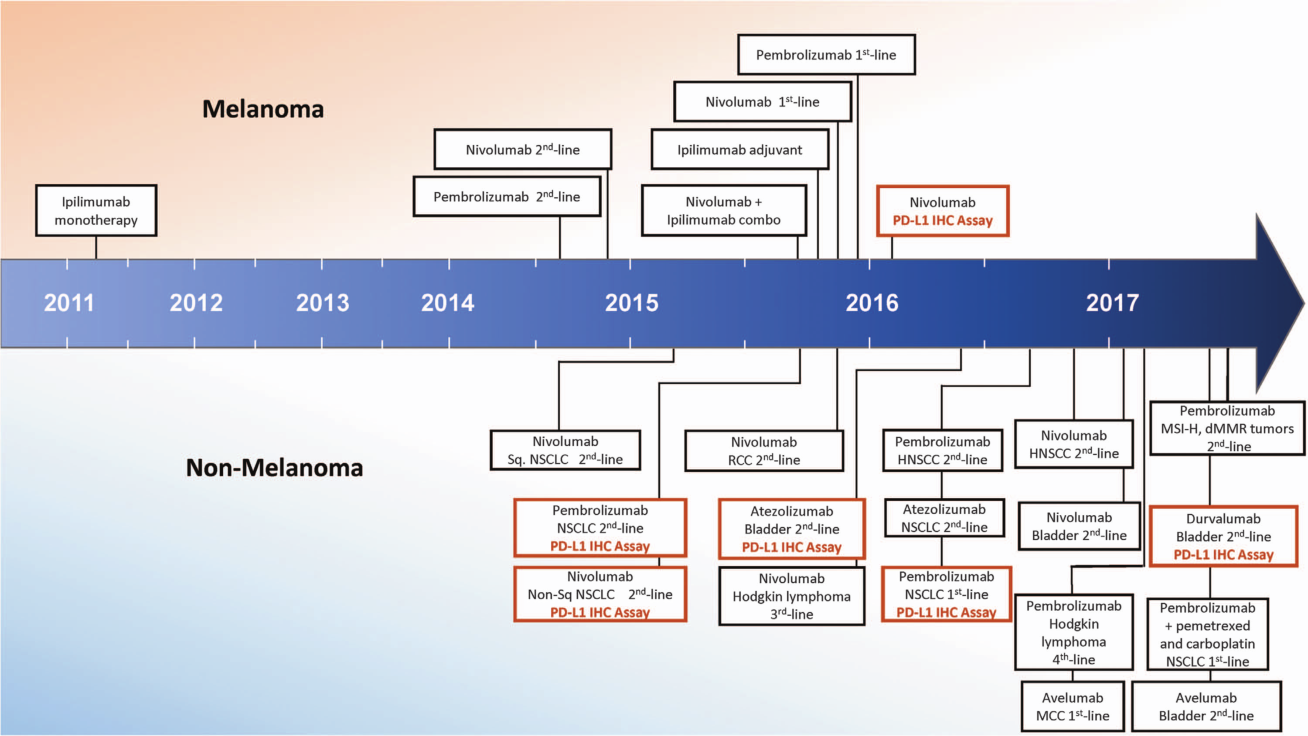
\includegraphics[width=1\linewidth]{figures-ext/02-timeline-immunotherapies} 

}

\caption[This timeline describes short history of FDA approval of checkpoint blocking immunotherapies up to 2017.]{\textbf{This timeline describes
short history of FDA approval of checkpoint blocking immunotherapies up
to 2017.} Reprinted by permission from Springer Nature
\citep{Taube2017a} Macmillan Publishers Limited, part of Springer
Nature. All Rights Reserved.}\label{fig:timeline-immunotherapies}
\end{figure}







The main drawback of immunotherapies is a heterogeneity of response
rate, which can vary i.e.~from 10--40\% in case of PD-L1blocking
\citep{Zou2016}, suggesting that some patients can have more chances
than others to respond to an immune therapy. So far, it has been shown
that anti PD-L1 therapies works more effectively in T cell infiltrated
tumors with exclusion of Tregs because of lack of difference in
expression of FOXP3 in responding and non-responding group of patients
\citep{Herbst2014}. Also some light has been shade by \citet{Rizvi2015}
who connected mutational rate of cancer cells to the chances of response
to an immunotherapy.

Despite those fundings, the precise qualifications of patients that
should be sensitive to an immunotherapy are not defined
\citep{Pitt2016}. As most patients do not answer to immunotherapies, it
stimulates researches to look for better biomarkers and patient
stratifications, and pharmaceutical industries to discover new immune
checkpoints based therapies.

\hypertarget{summary-of-the-chapter}{%
\section{Summary of the chapter}\label{summary-of-the-chapter}}

Cancer remains an important health problem of our era that touches many
people. Tumor cells are interacting with their mircoenvironement (called
Tumor Microenvironment (TME)) including normal cell, stroma cells and a
variety of immune cells. These cells can have a role in disease
progression and response to treatment. A modern approach to modulate TME
was proposed through application of immune therapies.

Many researches aim to link the composition and state of TME with
patients clinical features and survival. It has been shown that in some
cases certain cell types are beneficial to tumor development and some
are not. However a case by case approach of personalized medecine may be
necessary to fully understand the inter-patient heterogeneity.

A new way to classify cancers based on their TME is called
immunophenotyping. There is no well establish procedures to perform it
yet, but it can be integrated in the near future into the clinical
classification of tumors. It is a subject of active research to find new
biomarkers and signatures of different factors gouvening the TME. Lot of
interest is directed nowadays towards immune cells. Given that
traditional cell-type definitions can be questioned in the cancer
context, new cell states and functional subtypes are being redefined by
researchers.

There are many experimental techniques, as for instance immune staining
and FACS, that allow the in deep study of the immune system. They
require an important preparation steps and fresh samples. Also, a
limited number of variables can be observed through this techniques and
knowledge-based hypotheses are necessary. On the other hand,
high-throughput omic data allow to measure of the all system at the same
time as they can measure all referenced units (genes/methylaton sites/
copy number aberrations) from FFPE samples that can be stocked for a
long time. A discovery-type studies are then favoured and new biomarkers
can be discovered. Particularly suited for studying complex biological
systems is scRNA-seq as it provides gene expression profile of each cell
without a compulsory use of marker genes, indispensable in other
techniques to define cell-types. However, this technique remains quite
costly and it is not yet optimized.

Therefore to have very detailed system-level view of the TME with
traditional experimental techniques an uncountable amount of work and
resources would be necessary. Using omic techniques system approach is
possible, however to embrace fully the data complexity a computational
tools are needed. From data generation to analyzis different statistical
and mathematical challenges need to faced before arriving to valid
biological results and interpretations.

As I will present in the next chapter, in order to solve the problem of
extraction of cell-type heterogeneity from cancer bulk omic data, a
number of approaches was developed.

\hypertarget{methods}{%
\chapter{Mathematical foundation of cell-type deconvolution of
biological data}\label{methods}}

\chaptermark{Mathematical introduction}

In the previous chapter I presented state-of-art of the current
immuno-oncology research that has to embrace great complexity of cancer
disease and the immune system. One part of this complexity can be
explained by the presence and quantities of tumor-infiltrating immune
cells, their interactions with each other and the tumor.

In this chapter, I will discuss how mathematical models can be used to
extract information about different cell-types from `bulk' omics data or
how to de-mix mixed sources composing the bulk samples. To start with, I
will introduce you to basic concepts of machine learning. Then I will
focus on approaches adapted for cell-type deconvolution. In a literature
overview, I will depict the evolution of the field as well as discuss
the particularities of different tools for estimating presence and
proportion of immune cells within cancer bulk omic data.

\hypertarget{introduction-to-supervised-and-unsupervised-learning}{%
\section{Introduction to supervised and unsupervised
learning}\label{introduction-to-supervised-and-unsupervised-learning}}

Machine learning (ML) is a filed of computer science where system is
able to learn and improve given an objective function and the data.

A popular definition of machine learning has been given by Mitchell in
1997:

\begin{quote}
Machine learning: \emph{A computer program is said to learn from
experience E with respect to some class of tasks T and performance
measure P if its performance at tasks in T, as measured by P, improves
with experience E}.

--- Mitchell in 1997 \citep{Mitchell1997}
\end{quote}

Term \emph{Artificial intelligence} (AI) is often used by the media or
general public to describe machine learning. Indeed ML can be considered
as a branch of AI, together with computer vision and deep neural
networks applications. However, commonly ML and AI are used
interchangeably by the wide public.

ML is applied commonly in many fields of science and industry. I will
not discuss here a subtle differences between machine learning,
statistical learning, computational statistics and mathematical
optimisation.

In general, algorithms can be divided into groups given the application:

\begin{itemize}
\tightlist
\item
  classification - aims to assign observations to a group (discrete
  variable)
\item
  regression - aims to predict a continuous response of an input
  (continuous variable)
\item
  clustering - aims to divide data into groups that are related to each
  other based on a distance
\end{itemize}

Another important distinction can be made given the inputs to the
algorithm. Here, I present the differences between supervised and
unsupervised learning.

\hypertarget{supervised-learning}{%
\subsection{Supervised learning}\label{supervised-learning}}

Supervised learning can be described as ``the analysis of data via a
focused structure'' \citep{Piegorsch}. The main task is to predict an
output given the inputs. In the statistical language, the inputs are
often called the predictors or the independent variables. In the pattern
recognition literature the term features is preferred. The outputs are
called the responses, or the dependent variables. \citep{Hastie2009}

The initial data is divided into two sets: training and test. First the
model is trained with correct answers on the training data (learning to
minimise the error) , and then its performance is evaluated on the test
data.

Among widely used classifiers there are Support Vector Machines (SVM),
partition trees (and their extension random forests), and neural
networks. For regression it is common to encounter linear regression,
boosted trees regression,

\hypertarget{unsup}{%
\subsection{Unsupervised learning}\label{unsup}}

In Unsupervised learning is given the data and is asked to divide the
data given a certain constraint. However, the correct division of the
data is not known. Therefore an unsupervised algorithms aims to unveil
the ``hidden structure'' of the data, or latent variables.

One group of unsupervised learning are descriptive statistic methods,
such as: principal components, multidimensional scaling, self-organizing
maps, and principal curves. This methods aim to represent to the data
most adequately in low-dimensional space \citep{Hastie2009}.

Another group are clustering algorithms. Clustering is the way to create
groups (multiple convex regions) based on the intrinsic architecture of
the data. These groups are not necessarily known beforehand, but can
validated with the domain knowledge. Popular clustering algorithms are
knn, k-means, hierarchical clustering.

In both descriptive statistics and clustering, one important parameter
(often called \(k\)) is number to which we want to decompose the data
(number of factors, variables, clusters). Different algorithms and
applications can propose an automatic choice of \(k\) based on formal
indexes or previous knowledge, in others, user need to provide the
\(k\).

\hypertarget{low-dimensional-embeddingfor-visualization}{%
\subsection{Low-dimensional embedding~for
visualization}\label{low-dimensional-embeddingfor-visualization}}

There is a common confusion, often seen in computational biology,
between dimension reduction and clustering. This confusion is highly
pronounced with, a popular in biology, algorithm: T-distributed
Stochastic Neighbor Embedding (t-SNE) \citep{VanDerMaaten2008}. t-SNE
works in 2 main steps: (1) a~probability distribution~over pairs of
high-dimensional objects is computed in such a way that similar objects
have a high probability of being picked, whilst dissimilar points have
an extremely small probability of being picked, (2) t-SNE defines a
similar probability distribution over the points in the low-dimensional
map, and it minimizes the~Kullback--Leibler divergence between the two
distributions with respect to the locations of the points in the map. It
is not reliable to use t-SNE for clustering as it does not preserve
distances. It can also easily overfit the data and uncover `fake' or
`forced' patterns. Therefore, a clustering should not be applied to
t-sne reduced data. An alternative to t-SNE method is recently published
Uniform Manifold Approximation and Projection for Dimension Reduction
(UMAP) \citep{Mcinnes201}-- that is based on Laplacian eigenmaps, highly
scalable, reproducible and recently applied to biological data
\citep{Becht2018}. Older used alternatives are ISOMAPS (non linear
dimension reduction) or PCA (Principal components analysis). For any
non-linear dimension reduction method, it is not recommended to use
clustering \emph{a posteriori}. Clusters should be computed on original
data and then the cluster labels can be visualized in low-dimentional
embedding.

\hypertarget{section}{%
\section{}\label{section}}

\hypertarget{types-of-deconvolution}{%
\section{Types of deconvolution}\label{types-of-deconvolution}}

One specific application of mathematical/statistical tools is
deconvolution of mixed signals.

According to mathematical definition:

\begin{quote}
Deconvolution : \emph{the resolution of a convolution function into the
functions from which it was formed in order to separate their effects}
\end{quote}

Or in plain English:

\begin{quote}
\emph{a process of resolving something into its constituent elements or
removing complication}
\end{quote}

The similar problem of mixed sources can be encountered in other fields,
i.e.~signal processing, known also under the name of ``\textbf{cocktail
party problem}''. In the cocktail party problem, at a party with many
people and music, sound in recorded with several microphones. Through
blind source separation, it is possible to separate the voices of
different people and the musical background (Fig.
\ref{fig:cocktailparty}) \citep{Cherry1953}.

\begin{figure}

{\centering \includegraphics[width=1\linewidth]{figures-ext/cocktailparty} 

}

\caption[illutration of the cocktail party problem]{\textbf{Illutration of the cocktail party
problem}. During a cocktail party voices of participalnts can be
recorded with a set of microphones and then recovered though blind
source separation. Fot the illustration purposes only four sources are
mixed with three microphones, in reality the analysis can be performed
with many sources. However, number of samples (microphones) should be
higher than numer of sources (contrary to the illustration).}\label{fig:cocktailparty}
\end{figure}









The same concept can be transposed to the bulk omic data, each
biological species (like gene) is a cocktail party where each sample is
a microphone that gathers mixed signals of different nature. The signals
that form the mixtures can be different depending on the data type and
scientific question asked.

In general, the total bulk data can be split into three abundance
components \citep{Shen-Orr2013}:

\begin{enumerate}
\def\labelenumi{\arabic{enumi}.}
\tightlist
\item
  sample characteristic (disease, clinical features)
\item
  individual variation, genotype-specific or technical variation
\item
  presence and abundance of different cell types expressing set of
  characteristic genes
\end{enumerate}

Many scientists invested their efforts in order to dissect the bulk omic
data into interpretable biological components.

In scientific literature, there can be encountered three main
understanding of tumor deconvolution:

\begin{itemize}
\tightlist
\item
  \textbf{estimating clonality}: using genomic data is it possible to
  trace tumor phylogeny raised from mutations and aberrations in tumor
  cells; therefore it is dissecting \emph{intra}-tumor heterogeneity
  (i.e.~using transcriptomic data \citep{Schwartz2015}, or more often
  CNA data (see \protect\hyperlink{otherDecon}{Section X})
\item
  \textbf{estimating purity}: deconvolution into tumor and immune/stroma
  compartments, often aiming to ``remove'' not-tumor signal from the
  expression data, can be performed with different data types, the most
  reliable estimations are obtained usually from CNA data (see
  \protect\hyperlink{otherDecon}{Section X})
\item
  \textbf{estimating cell-type} proportions and/or profiles from bulk
  omics data, most of works were performed on transcriptome data (see
  \protect\hyperlink{cellTypeTrans}{Section A}) and some on the
  methylome data (see \protect\hyperlink{otherDecon}{Section X})
\end{itemize}

These three types of deconvolution can be performed on the bulk omics
data. Here we will focus on cell-type deconvolution models using bulk
transcriptome. I will also briefly introduce deconvolution models
applied to other data types (methylome and CNA).

\hypertarget{cellTypeTrans}{%
\section{Cell-type deconvolution of bulk
transcriptomes}\label{cellTypeTrans}}

The idea of un-mixing the bulk omic profiles is documented to first
appear in an article of \citet{Venet2001} as a way to

\begin{quote}
\emph{infer the gene expression profile of the various cellular types
(\ldots{}) directly from the measurements taken on the whole sample}
\end{quote}

In the basic hypothesis \citep{Abbas2009}, mixture of signals from TME
in transcriptomic samples can be described as a linear mixture.

\begin{equation} 
X = SA  \label{eq:linear}
\end{equation}

\eqref{eq:linear}

Where in Equaltion \eqref{eq:linear} \(X\) is microarray data matrix of
one biological sample, \(A\) are mixing proportions and \(S\) is the
matrix of expression of genes in each cell type.

Algebraically the same problem can be formalized as latent variable
model:

\begin{equation} 
\begin{aligned}
\forall i \in \{1,M\},  \forall  j \in \{1,N\} \\
x_{ij}= \sum_{k=1}^K a_{kj} *s_{ik}+ e_{ij} \label{eq:algebraic}
\end{aligned}
\end{equation}

Where \(x_{ij}\) is expression of gene \(i\) in sample \(j\), \(a_{kj}\)
is the proportion of cell type \(k\) in sample \(j\) and \(s_{ik}\) is
the expression of the gene \(i\) in the cell type \(k\), \(K\) total
number of cell types, \(N\) total number of samples, \(M\) total number
of genes. The error term \(e_{ij}\) cannot be directly measured.

The goal of deconvolution is to reverse these equations and starting
from the mixture infer the \(A\) (or \(a_{kj}\)) and \(S\) (or
\(s_{ik}\)).

Graphically the deconvolution of bulk gene expression can be depicted as
in Fig. \ref{fig:deconvolution-cartoon}.

\begin{figure}

{\centering 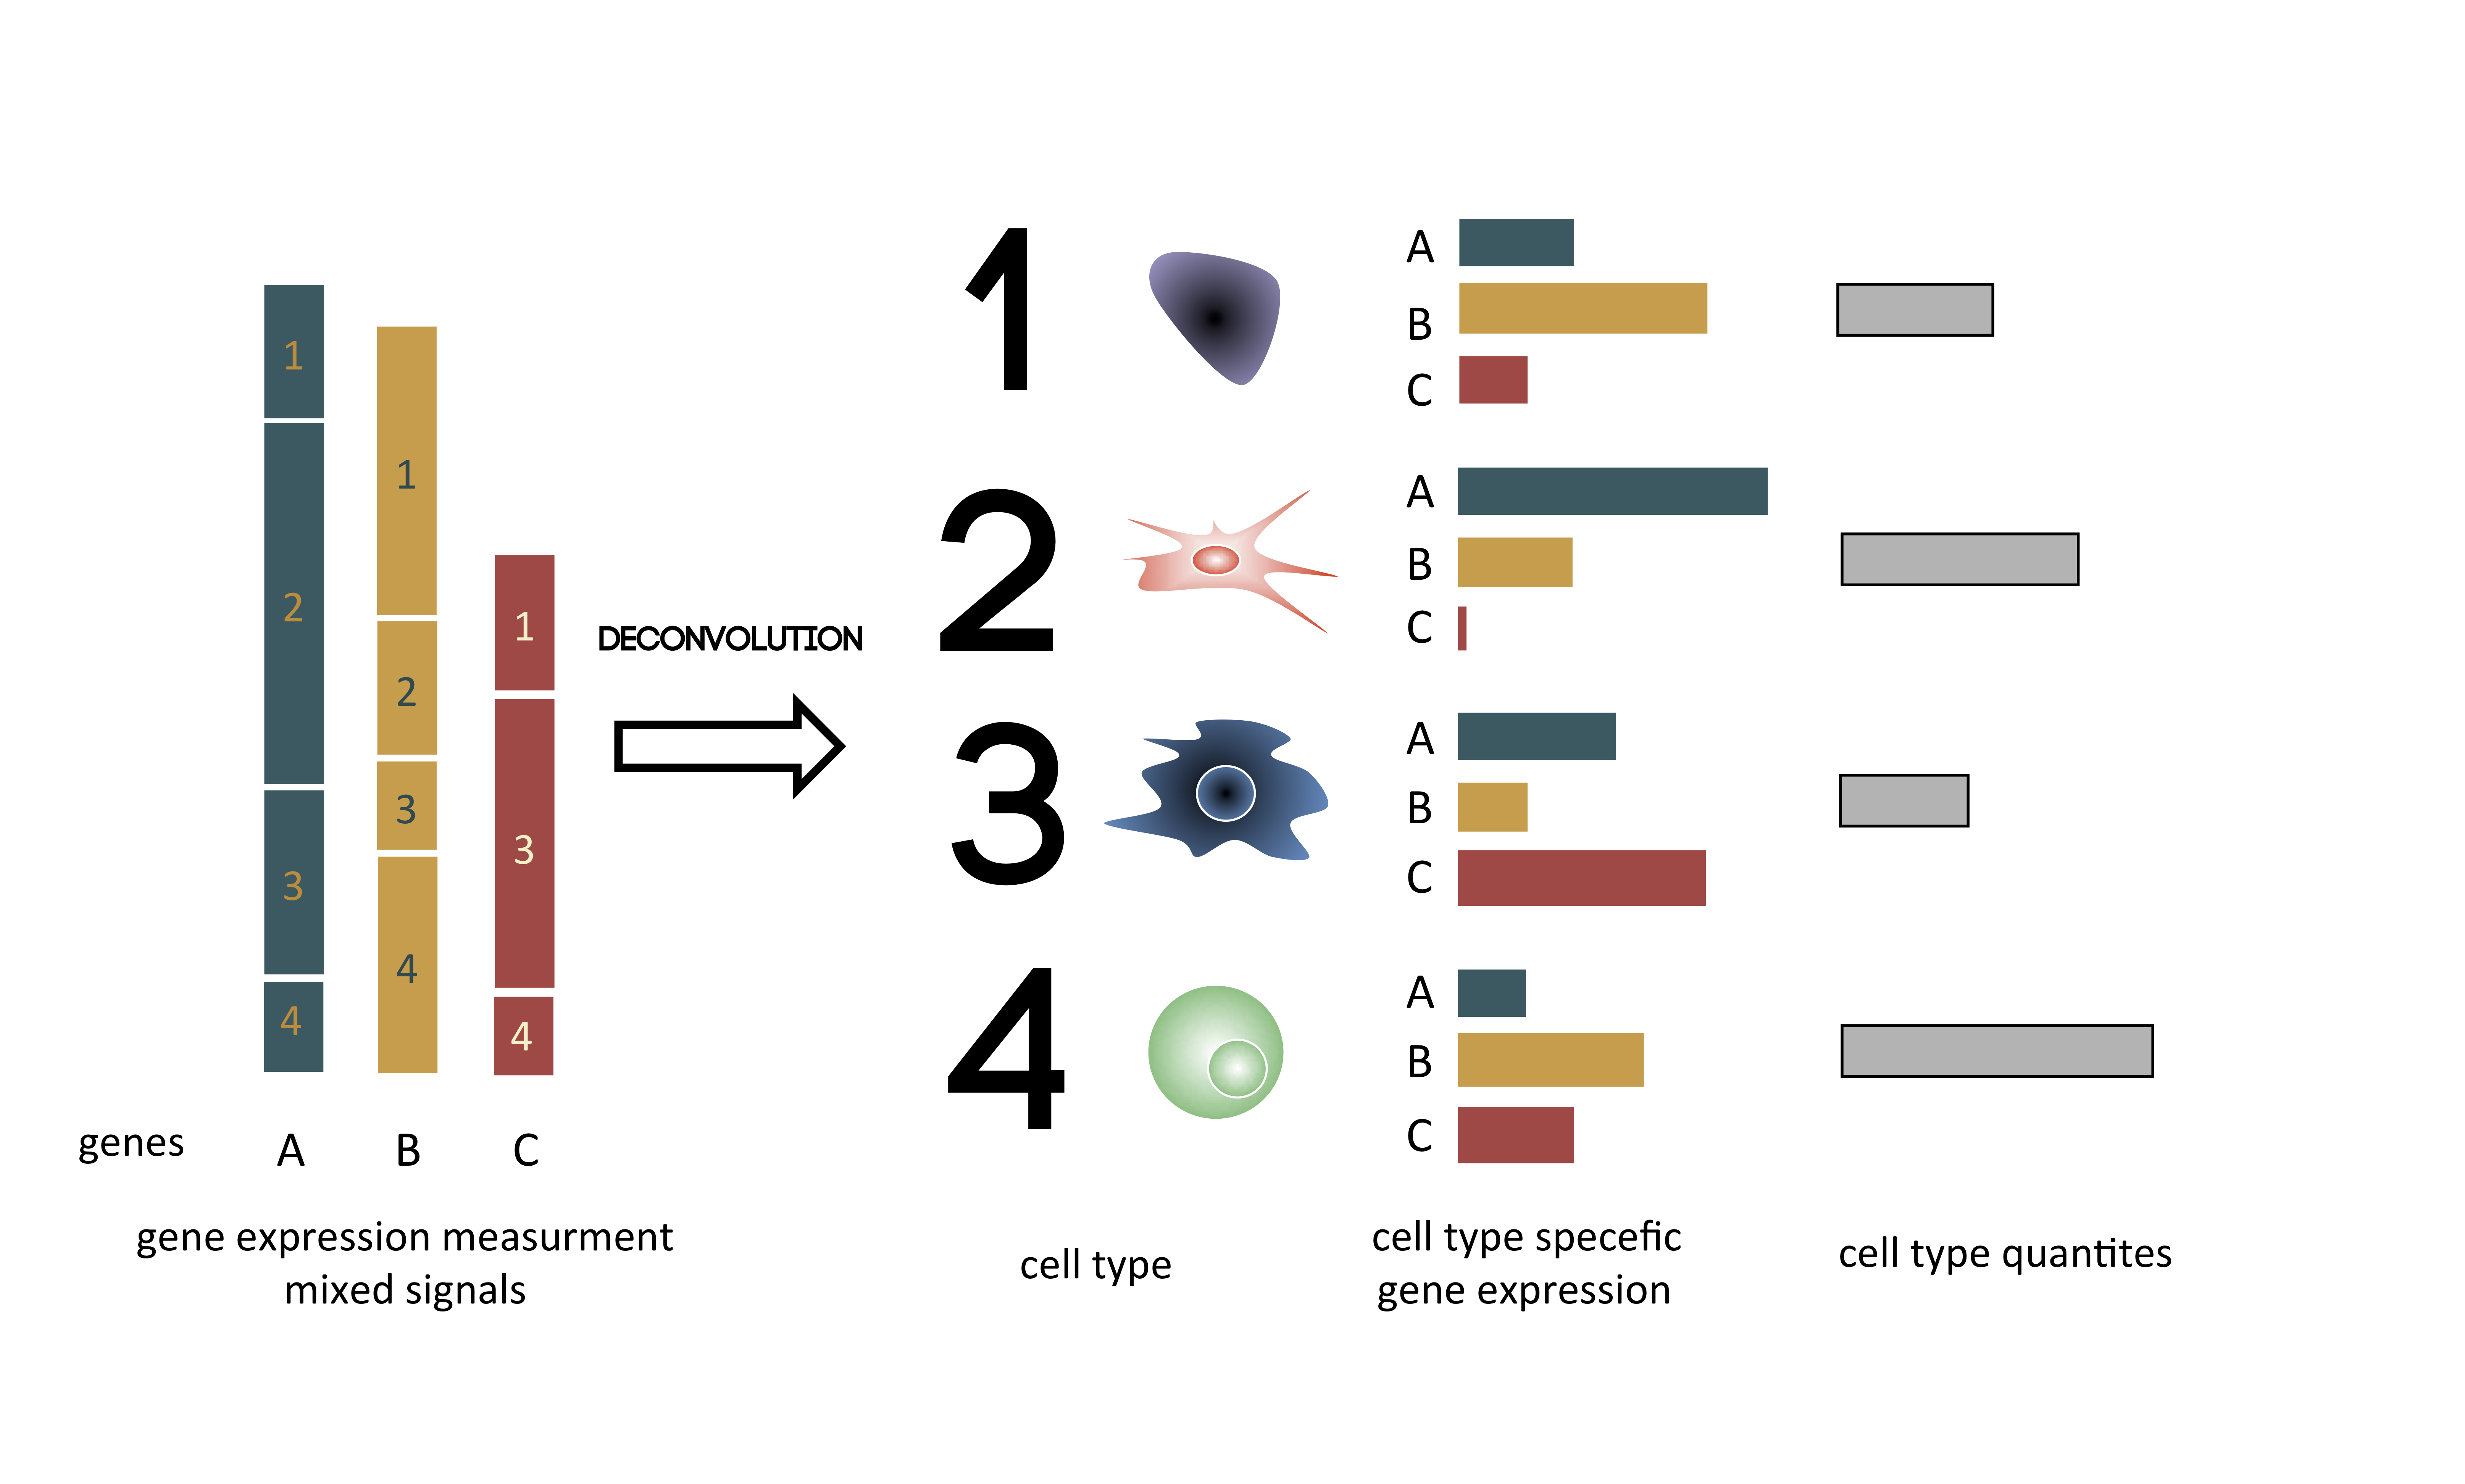
\includegraphics[width=1\linewidth]{figures-ext/deconv} 

}

\caption[Principle of the deconvolution applied to transcriptome]{\textbf{Principle of the
deconvolution applied to transcriptome} Graphical illustration of the
deconvolution of mixed samples. Starting from the left, gene expression
of genes A B C is a sum of expression of cell types 1, 2, 3, 4. After
deconvolution, cell types are separated and gene expression of each cell
type is estimated taking into account cell type proportions.}\label{fig:deconvolution-cartoon}
\end{figure}








However, in this model, either the mixing proportions, number of mixing
sources or an array of specific genes need to be know. While, in the
real-life case, only \(X\) is truly known. Therefore, developed models
proposed various manners for estimating number of mixing sources and
their proportions, or the specific cell type expression.

Why there is a need for cell-type deconvolution approaches?

\begin{itemize}
\item
  for differential gene expression analysis, to avoid confusion between
  a feature and cell-type abundance
\item
  difference in gene expression in one cell type can be blurred by
  presence of other cells expressing the gene
\item
  to obtain information about a fraction of given component in the
  sample
\item
  to infer context-specific profile or signature
\end{itemize}

\hypertarget{literature-overview}{%
\subsection{Literature overview}\label{literature-overview}}

In order to answer general and specific need for cell-type deconvolution
of bulk transcriptomes researches produced a large collection of tools.
I have collected all (to my knowledge) articles published in journals or
as a pre-print (up to May 2018) that propose original models/tools of
cell-type deconvolution of bulk \textbf{transcriptomes} (Tab.
\ref{tab:mytab}). Therefore clonal deconvolution methods are not
included in this overview. The transcriptome-based purity estimation
methods are included as many of them proposed an initial 2-sources model
that could be, at least in theory, extended to multiple sources model.
Also, I did not included cell-type deconvolution methods of other data
types (such as methylome). A separate (section X){[}\#otherDecon{]} is
dedicated to non-transcriptome methods.

\begin{landscape}\rowcolors{2}{gray!6}{white}
\begin{table}

\caption[Summary of methods for cell-type deconvolution of bulk transcriptome]{\label{tab:mytab}\textbf{Summary of methods for cell-type
deconvolution of bulk transcriptome}. Data gathered based on pubmed and
google scholar search in May 2018.}
\centering
\resizebox{\linewidth}{!}{
\begin{tabular}[t]{cccccccccccccc}
\hiderowcolors
\toprule
name & data & type & doi & year & application & availability & out.profiles & out.proportions & category & language & citations & pop.index & previously.covered\\
\midrule
\showrowcolors
GSVA scores & RNA-seq & supervised & https://doi.org/10.1158/1078-0432.CCR-17-3509 & 2018 & Cancer transcriptome & NA & FALSE & TRUE & enrichment & unknown & 1 & 1.00 & FALSE\\
MySort & MA & supervised & https://doi.org/10.1186/s12859-018-2069-6 & 2018 & Blood & https://testtoolshed.g2.bx.psu.edu/repository?repository\_id=6e9a9ab163e578e0\&changeset\_revision=e3afe097e80a & FALSE & TRUE & regression & R, web tool & 0 & 0.00 & FALSE\\
ADVOCATE & RNA-seq & supervised & https://doi.org/10.1101/288779 & 2018 & Cancer transcriptome & NA & TRUE & TRUE & probabilistic & R & 0 & 0.00 & FALSE\\
DTD & scRNA-seq & supervised & https://arxiv.org/abs/1801.08447v1 & 2018 & Cancer transcriptome & NA & FALSE & TRUE & regression & unknown & 0 & 0.00 & FALSE\\
CellDistinguisher & MA + RNA-seq & unsupervised & https://doi.org/10.1371/journal.pone.0193067 & 2018 & yeast cell cycle & https:// github.com/GeneralElectric/CcellDdistinguisher & TRUE & TRUE & convex hull & R & 0 & 0.00 & FALSE\\
\addlinespace
dtangle & MA + RNA-seq & supervised & https://doi.org/10.1101/290262 & 2018 & Blood & https://cran.r-project.org/package=dtangle & FALSE & TRUE & regression & R & 0 & 0.00 & FALSE\\
DeconICA & MA + RNA-seq & unsupervised & https://doi.org/10.5281/zenodo.1250069 & 2018 & Cancer transcriptome & https://urszulaczerwinska.github.io/DeconICA/ & TRUE & TRUE & matrix factorisation & R, matlab & 0 & 0.00 & FALSE\\
xCell & MA + RNA-seq & supervised & https://dx.doi.org/10.1186\%2Fs13059-017-1349-1 & 2017 & Cancer transcriptome & http://xcell.ucsf.edu/; https://github.com/dviraran/xCell & FALSE & TRUE & enrichment & R, web tool & 15 & 7.50 & FALSE\\
BioQC & MA + RNA-seq & supervised & https://doi.org/10.1186/s12864-017-3661-2 & 2017 & Gene expression & https://www.bioconductor.org/packages/release/bioc/html/BioQC.html & FALSE & FALSE & enrichment & R & 6 & 3.00 & TRUE\\
EPIC & RNA-seq & supervised & https://dx.doi.org/10.7554\%2FeLife.26476 & 2017 & Cancer transcriptome & https://github.com/GfellerLab/EPIC & FALSE & TRUE & regression & R & 4 & 2.00 & FALSE\\
\addlinespace
Estimation of immune cell content & scRNA-seq & supervised & https://doi.org/10.1038/s41467-017-02289-3 & 2017 & Cancer transcriptome & NA & FALSE & TRUE & regression & unknown & 3 & 1.50 & FALSE\\
Enumerateblood & MA & supervised & https://doi.org/10.1186/s12864-016-3460-1 & 2017 & Blood gene expression & https://github.com/cashoes/enumerateblood & TRUE & TRUE & probabilistic & R & 2 & 1.00 & TRUE\\
ImmunoStates & MA & supervised & https://doi.org/10.1101/206466 & 2017 & Blood, solid tissue, disease & NA & FALSE & TRUE & regression & R & 1 & 0.50 & FALSE\\
quanTIseq & RNA-seq + Images & supervised & https://doi.org/10.1101/223180 & 2017 & Cancer transcriptome & http://icbi.at/software/quantiseq/doc/index.html & FALSE & TRUE & regression & web tool & 1 & 0.50 & FALSE\\
SMC & MA & unsupervised & https://doi.org/10.1371/journal.pone.0186167 & 2017 & Tissue mixtures & https://github.com/moyanre/smcgenedeconv & TRUE & TRUE & probabilistic & matlab & 1 & 0.50 & FALSE\\
\addlinespace
Modular discrimination index & MA + RNA-seq & supervised & https://doi.org/10.1371/journal.pone.0169271 & 2017 & Skin tuberculosis & https://github.com/MJMurray1/MDIScoring & FALSE & TRUE & enrichment & R & 1 & 0.50 & FALSE\\
DemixT & MA + RNA-seq & supervised & https://doi.org/10.1101/146795 & 2017 & Cancer transcriptome & https://github.com/wwylab/DeMixT & TRUE & TRUE & probabilistic & R & 0 & 0.00 & FALSE\\
Post‐modified non‐negative matrix factorization & RNA-seq & unsupervised & https://doi.org/10.1002/cem.2929 & 2017 & Cancer transcriptome & NA & TRUE & TRUE & matrix factorisation & matlab & 0 & 0.00 & FALSE\\
Infino & RNA-seq & supervised & https://doi.org/10.1101/221671 & 2017 & Cancer transcriptome & https://github.com/hammerlab/infino & TRUE & TRUE & probabilistic & Stan & 0 & 0.00 & FALSE\\
MCPcounter & MA & supervised & https://doi.org/10.1186/s13059-016-1070-5 & 2016 & Cancer transcriptome & https://github.com/ebecht/MCPcounter & FALSE & TRUE & enrichment & R & 42 & 14.00 & TRUE\\
\addlinespace
ssGSEA applied to renal cell
carcinoma & RNA-seq & supervised & https://doi.org/10.1186/s13059-016-1092-z & 2016 & Cancer transcriptome & NA & FALSE & TRUE & enrichment & R & 40 & 13.33 & TRUE\\
CAM & MA & unsupervised & https://doi.org/10.1038/srep18909 & 2016 & yeast cell cycle & http://mloss.org/software/view/437, & TRUE & TRUE & convex hull & R-java & 12 & 4.00 & TRUE\\
Immune  Quant & undefined & supervised & https://doi.org/10.1093/bioinformatics/btw535 & 2016 & Human tissues & http://csgi.tau.ac.il/ImmQuant/ & FALSE & TRUE & regression & web tool & 5 & 1.67 & TRUE\\
VoCAL & MA, GWAS & supervised & https://doi.org/10.1371/journal.pcbi.1004856 & 2016 & Lung tissue & https://cran.r-project.org/web/packages/ComICS/index.html & FALSE & TRUE & regression & R & 5 & 1.67 & TRUE\\
CellMapper & MA & semi-supervised & https://doi.org/10.1186/s13059-016-1062-5 & 2016 & Brain tissue & http://bioconductor.org/packages/release/bioc/html/CellMapper.html & TRUE & FALSE & matrix factorisation & R & 5 & 1.67 & TRUE\\
\addlinespace
contamDE & RNA-seq & supervised & https://doi.org/10.1093/bioinformatics/btv657 & 2016 & Tumor purity & https://github.com/zhanghfd/contamDE/ & TRUE & TRUE & probabilistic & R & 4 & 1.33 & TRUE\\
ImSig & RNA-seq & supervised & https://doi.org/10.1101/077487 & 2016 & Cancer transcriptome & NA & FALSE & TRUE & enrichment & unknown & 0 & 0.00 & FALSE\\
CIBERSORT & MA & supervised & https://doi.org/10.1038/nmeth.3337 & 2015 & Cancer transcriptome & http://cibersort.stanford.edu/ & FALSE & TRUE & regression & R, web tool & 343 & 85.75 & TRUE\\
Virtual Microdissection & MA & supervised & https://doi.org/10.1038/ng.3398 & 2015 & detection of cancer and stroma in PDAC (TCGA) & NA & TRUE & TRUE & matrix factorisation & matlab & 86 & 21.50 & TRUE\\
CellCODE & MA & semi-supervised & https://doi.org/10.1093/bioinformatics/btv015 & 2015 & Blood & http://www.pitt.edu/\textasciitilde{}mchikina/CellCODE/ & TRUE & TRUE & matrix factorisation & R- C-C++- Fortran & 28 & 7.00 & TRUE\\
\addlinespace
CoD & RNA-seq & supervised & https://doi.org/10.1093/bioinformatics/btv498 & 2015 & Mice diseased tissues & http://www.csgi.tau.ac.il/CoD/ & FALSE & TRUE & regression & web tool & 4 & 1.00 & TRUE\\
DCQ & RNA-seq & supervised & https://dx.doi.org/10.1002\%2Fmsb.134947 & 2014 & Mice blood under flu infection & http://www.dcq.tau.ac.il/ & FALSE & TRUE & regression & web tool & 32 & 6.40 & TRUE\\
UNDO & MA & unsupervised & https://doi.org/10.1093/bioinformatics/btu607 & 2014 & Cancer transcriptome & https://www.bioconductor.org/packages/release/bioc/html/UNDO.html & TRUE & TRUE & matrix factorisation & R & 18 & 3.60 & TRUE\\
ESTIMATE & MA + RNA-seq & supervised & https://doi.org/10.1038/ncomms3612 & 2013 & Cancer transcriptome & https://sourceforge.net/projects/estimateproject/ & FALSE & TRUE & enrichment & R & 266 & 44.33 & TRUE\\
DeconRNASeq & RNA-seq & supervised & https://doi.org/10.1093/bioinformatics/btt090 & 2013 & Tissue mixtures & https://www.bioconductor.org/packages/release/bioc/html/DeconRNASeq.html & FALSE & TRUE & regression & R & 52 & 8.67 & TRUE\\
\addlinespace
DSA & MA & supervised & https://dx.doi.org/10.1186\%2F1471-2105-14-89 & 2013 & Cancer transcriptome & https://github.com/zhandong/DSA & TRUE & TRUE & regression & R & 52 & 8.67 & TRUE\\
ISOpure & MA & supervised & https://doi.org/10.1186/gm433 & 2013 & Cancer transcriptome & https://qlab.faculty.ucdavis.edu/isopure/ & TRUE & TRUE & probabilistic & matlab, R & 44 & 7.33 & TRUE\\
DeMix & MA & supervised & https://doi.org/10.1093/bioinformatics/btt301 & 2013 & Cancer purity & http://odin.mdacc.tmc.edu/∼wwang7/DeMix.html. & TRUE & TRUE & probabilistic & C, R & 38 & 6.33 & TRUE\\
Nanodissection & MA & supervised & https://doi.org/10.1101/gr.155697.113 & 2013 & Chronic kidney disease (Cell lineages) & http://nano.princeton.edu/ & FALSE & TRUE & regression & web tool & 33 & 5.50 & TRUE\\
TIMER & MA + RNA-seq & supervised & https://doi.org/10.1186/s13059-016-1028-7 & 2013 & Cancer transcriptome & http://cistrome.org/TIMER/ & FALSE & TRUE & regression & web tool & 33 & 5.50 & TRUE\\
\addlinespace
Self-directed Method for Cell-Type Identification & MA & unsupervised & https://doi.org/10.1371/journal.pcbi.1003189 & 2013 & Cancer transcriptome & NA & TRUE & TRUE & matrix factorisation & matlab & 18 & 3.00 & TRUE\\
MMAD & MA & BOTH & https://doi.org/10.1093/bioinformatics/btt566 & 2013 & in vitro tissue mlxtures & http://sourceforge.net/projects/mmad/ & TRUE & TRUE & regression & matlab & 11 & 1.83 & TRUE\\
Statical mechanics approach & undefined & unsupervised & https://arxiv.org/abs/1210.7508v1 & 2013 & Udefined & NA & TRUE & TRUE & probabilistic & unknown & 2 & 0.33 & FALSE\\
TEMT & RNAseq & supervised & https://bmcbioinformatics.biomedcentral.com/articles/10.1186/1471-2105-14-S5-S11 & 2013 & in vitro cell mixtures & https://github.com/uci-cbcl/TEMT & FALSE & TRUE & probabilistic & python & 0 & 0.00 & TRUE\\
Semi-supervised Nonnegative Matrix Factorization & MA & semi-supervised & https://doi.org/10.1016/j.meegid.2011.08.014 & 2012 & Blood & https://web.cbio.uct.ac.za/\textasciitilde{}renaud/CRAN/web/CellMix/ & TRUE & TRUE & matrix factorisation & R & 61 & 8.71 & TRUE\\
\addlinespace
PERT & MA & supervised & https://doi.org/10.1371/journal.pcbi.1002838 & 2012 & blood & https://github.com/gquon/PERT & TRUE & TRUE & probabilistic & octave & 33 & 4.71 & TRUE\\
CTen & MA & supervised & https://doi.org/10.1186/1471-2164-13-460 & 2012 & Infected lung tissue & http://www.influenza-x.org/\textasciitilde{}jshoemaker/cten/ & TRUE & FALSE & enrichment & web tool & 31 & 4.43 & TRUE\\
PSEA & MA & supervised & https://doi.org/10.1038/nmeth.1710 & 2011 & Brain tissue & https://bioconductor.org/packages/release/bioc/html/PSEA.html & FALSE & TRUE & regression & R & 96 & 12.00 & TRUE\\
Quadratic programming & MA & supervised & https://doi.org/10.1371/journal.pone.0027156 & 2011 & Blood & NA & FALSE & TRUE & regression & unknown & 76 & 9.50 & TRUE\\
SPEC & MA & supervised & https://doi.org/10.1186/1471-2105-12-258 & 2011 & Blood & http://clip.med.yale.edu/SPEC/ & FALSE & TRUE & enrichment & R & 39 & 4.88 & TRUE\\
\addlinespace
csSAM & MA & supervised & https://doi.org/10.1038/nmeth.1439 & 2010 & Blood & https://github.com/shenorrLab/csSAM & TRUE & FALSE & regression & R & 286 & 31.78 & TRUE\\
Statistical expression deconvolution & MA & supervised & https://doi.org/10.1093/bioinformatics/btq097 & 2010 & Cancer xenografts & NA & FALSE & TRUE & regression & unknown & 53 & 5.89 & TRUE\\
DSection & MA & supervised & https://doi.org/10.1093/bioinformatics/btq406 & 2010 & Tissue mixtures & http://informatics.systemsbiology.net/DSection & TRUE & FALSE & probabilistic & matlab & 52 & 5.78 & TRUE\\
deconf & MA & unsupervised & https://doi.org/10.1186/1471-2105-11-27 & 2010 & Blood & https://static-content.springer.com/esm/art\%3A10.1186\%2F1471-2105-11-27/MediaObjects/12859\_2009\_3484\_MOESM1\_ESM.ZIP & TRUE & TRUE & matrix factorisation & R & 41 & 4.56 & TRUE\\
Abbas regression & MA & supervised & https://doi.org/10.1371/journal.pone.0006098 & 2009 & Blood & NA & FALSE & TRUE & regression & R & 207 & 20.70 & TRUE\\
\addlinespace
ISOLATE & MA & supervised & https://dx.doi.org/10.1093\%2Fbioinformatics\%2Fbtp378 & 2009 & Cancer transcriptome & https://qlab.faculty.ucdavis.edu/isolate/ & TRUE & TRUE & matrix factorisation & matlab & 37 & 3.70 & TRUE\\
Electronical substraction & MA & supervised & https://doi.org/10.1093/bioinformatics/btm508 & 2007 & Infected macrophages & NA & TRUE & TRUE & regression & unknown & 30 & 2.50 & TRUE\\
Computational expression deconvolution & MA & supervised & https://doi.org/10.1186/1471-2105-7-328 & 2006 & Murine mammary gland & NA & FALSE & TRUE & regression & unknown & 36 & 2.77 & TRUE\\
Robust Computational Reconstitution & MA & supervised & https://doi.org/10.1186/1471-2105-7-369 & 2006 & Synovial tissue (cell types in silico) & NA & FALSE & TRUE & regression & unknown & 6 & 0.46 & TRUE\\
MHMM & MA & unsupervised & https://doi.org/10.1089/cmb.2006.13.1749 & 2006 & Yeast cell cycle & NA & TRUE & TRUE & probabilistic & unknown & 4 & 0.31 & TRUE\\
\addlinespace
In silico microdissection & MA & unsupervised & https://doi.org/10.1186/1471-2105-6-54 & 2005 & In vitro tissue mixtures & NA & TRUE & TRUE & probabilistic & unknown & 45 & 3.21 & TRUE\\
Mixture models & MA & supervised & https://doi.org/10.1093/bioinformatics/bth139 & 2004 & Cancer transcriptome & broken link & TRUE & TRUE & probabilistic & R & 66 & 4.40 & TRUE\\
DECONVOLUTE & MA & supervised & https://doi.org/10.1073/pnas.1832361100 & 2003 & yeast cell cycle & broken link & FALSE & TRUE & regression & Java 2 & 135 & 8.44 & TRUE\\
Direct method & MA & unsupervised & https://www.ncbi.nlm.nih.gov/pubmed/11473019 & 2001 & cander and normal tissue & NA & TRUE & TRUE & matrix factorisation & unknown & 96 & 5.33 & TRUE\\
\bottomrule
\end{tabular}}
\end{table}
\rowcolors{2}{white}{white}
\end{landscape}





The Table \ref{tab:mytab} contains 64 (including mine) deconvolution
methods. It can be observed (Fig. \ref{fig:pubyear}) that since the
begging of my thesis (2015) the number of publications has doubled (64
publications in 2018 vs.~33 in 2014). Also, since 2014 more methods are
published every year. In Fig. \ref{fig:pubyear} \emph{hallmark}
publications are indicated in red above their year of publication. The
three most popular methods (based of number of citations/number of years
since publication) are CIBERSORT \citep{Newman2015} (2015, total number
of citations: 343 and 88.75 citations per year), ESTIMATE
\citep{Yoshihara2013} (2013, total number of citations: 266 and 44.33
citations per year), and csSAM \citep{ShenOrr2010} (2010, total number
of citations: 286 and 31.77 citations per year). It can be noticed that
the high impact of the journal plays a role, the top 3 cited methods
were published in \emph{Nature Methods} and \emph{Nature Communications}
followed by Virtual Microdissection method \citep{Moffitt2015} (2015)
published in \emph{Nature Genetics}. However, the fifth most cited
publication \citet{Abbas2009} (2009, total of 207 citations) appeared in
\emph{PLOS ONE}. As the index is a bit penalizing for recent
publications, among commonly cited tools after 2015 are MCPcounter with
42 citations (2016, 32 without self-citations) and xCell with 14
citations (2017, 11 without self-citations). A big number of
publications with low number of citations were published in \emph{Oxford
Bioinformatics} or \emph{BMC Bioinformatics} which underlines importance
of publishing a computational tool along with an important biological
message rather than in a technical journal in order to increase a chance
to be used by other researchers.

Another important aspect is availability of the tool. One-third (in
total 21) methods do not provide source code or a user-interface tool to
reproduce their results. Among those articles, 13 was published before
2015. Therefore, it can be concluded that the pressure of publishers and
research community on reproducibility and accessibility of bioinformatic
tools gives positive results. \citet{Shen-Orr2013}, authors of
semi-supervised NMF method \citep{Gaujoux2012}, published \emph{CellMIx:
a comprehensive toolbox for gene expression deconvolution} where he
implements most of previously published tools in R language and group
them in the same R-package. This work tremendously increased the
usability of previously published deconvolution methods. The CellMix
package is one of the state-of-the-art work on deconvolution that
regroups algorithms, signatures and benchmark datasets up to 2013.

The most popular language of implementation of published methods is R
(49.2 \%), followed by Matlab (11.11\%), only one tool so far was
published in Python.

Also, most of methods were designed to work with microarray data. There
is a high chance that some of them are adaptable to RNA-seq. However,
little number of older methods was tested in a different setup. For some
method, as CIBERSORT, demonstrated to work with microarray and applied
commonly to RNA-seq by other researchers, the validity of results
remains unclear as some studies claim that CIBERSORT performs accurately
applied to RNA-seq \citep{Thorsson2018} and other opt agains it
(\citet{Li2017}; \citet{Tamborero2018}). Most of newer methods
(i.e.~EPIC \citep{Racle2017}, quanTIseq \citep{Finotello2017} or Infino
\citep{Zaslavsky2017}) are specifically designed for RNA-seq
TPM-normalized data. Some methods, mostly enrichment-based methods, are
applicable to both technologies (i.e.~xCell \citep{Aran2017}).

It is remarkable that the general aim of the cell-type deconvolution
changed with time. The earlier methods aimed to improve the power of
differential expression analysis though \emph{purification} of the gene
expression. For example, to compare differentially expressed genes (DEG)
in T-cell from the blood in two conditions. However, the obtained
purified profiles from complex mixtures were often uncertain
\citep{Onuchic2016}. Recently, the most mentioned goal of deconvolution
is quantification of proportions of different cell types, especially in
the context of cancer transcriptomes motivated by redefinition of
immunophenotypes discussed in the previous chapter. The most popular
tissue of interest for deconvolution algorithms are cancer tissues and
blood, other applications are cell-cycle time dependent fluctuations of
yeast, brain cells and glands .

Mathematically speaking, I have divided methods into four categories:
probabilistic, regression, matrix factorisation and convex hull
depending on the nature of approach. Most of the methods (48 - 74.6\%)
are working within a supervised framework and only 20\% (14) are
unsupervised. The approaches will be described in detail in the
following section.

There are numerous practical differences between the methods.
\citet{Shen-0rr2013} in his review of deconvolution tools, grouped the
tools depending on their inputs and outputs. Given type of outputs
deconvolution can be considered as complete (proportions and cell
profiles) or partial (one of those). Moreover, the inputs of the
algorithms can be important to evaluate how practical the tool is. The
most popular tools and the most recent tools ask minimal input from the
user: the bulk gene expression matrix, or even raw sequencing data
\citep{Finotello2017}. Older methods usually request either at least
approximative proportions of mixed cells or purified profiles to be
provided. The newer methods include the reference profiles in the tool
if necessary. Some tools, including most of purity estimation tools,
demand an additional data input as normal samples or another data type
such as CNA data (Timer \citep{Li2013}, VoCAL \citep{Steuerman2016}{]}
or image data (quanTIseq \citep{Finotello2017}). An important parameter
is also a number of sources (\(k\)) to which the algorithm deconvolutes
the mixture. In many methods it should be provided by the user, which
can be difficult in a case of complex mixtures of human tissues. In
addition, type of method can also limit the number of sources, for
example, a probabilistic framework privilege lower number of sources
(2-3) due to the theoretical constraints. In regression depending on
provided reference the output number of estimated sources is imposed.
Because of the problem of collinearity and similarity of immune cell
profiles, it is hard to distinguish between cell sub-types,
deconvolution into fine-grain cell subtypes is often called often deep
deconvolution. Some methods (i.e.~CIBERSORT, Infino, xCell) give a
specific attention to deconvolution of cell-subtypes. An absolute
presence of a cell type in the mixture can be also an important factor,
if it is too low it can reach a detection limit, Electronic subtraction
\citep{Gosink2007} discuss specifically the detection of rare cel-types.

Running time and necessary infrastructure are another way to
characterize the methods. Although it is hard to compare objectively the
running time simultaneously of all the tools because of the
heterogeneity of methods and different datasets analysed, some
tendencies can be observed. If one thinks about applying deconvolution
methods to big cohorts, regression and enrichment-based methods should
be well suited. As far as matrix factorisation is concerned, it is
depending on implementation (i.e.~R vs Matlab) and if number of sources
needs to be estimated (multiple runs for different \(k\) parameter) or
if a stabilisation needs to applied (multiple runs for the same \(k\)
parameter). Finally, probabilistic tools seem to be difficult to scale,
i.e.~authors of Infino admit that their pipeline is not yet applicable
at high-throughput.

In order to let user better understand the differences between different
mathematical approaches, I will introduce shortly the types of
approaches used for cell-type deconvolution of transcriptomes as well as
their strong and weak points.

\begin{figure}

{\centering 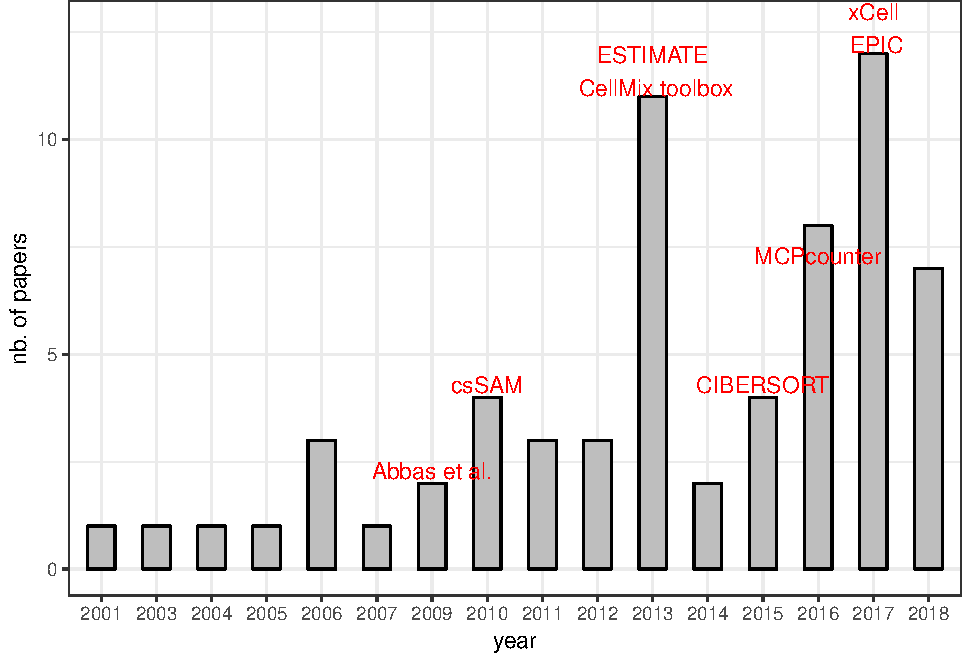
\includegraphics[width=0.7\linewidth]{UCzPhDThesis_files/figure-latex/pubyear-1} 

}

\caption[Distribution of publications of cell-type deconvolution of bulk transcriptome over the years]{\textbf{Distribution of publications of cell-type
deconvolution of bulk transcriptome over the years}. In red: hallmark
publications. Data gathered based on pubmed and google scholar search in
May 2018.}\label{fig:pubyear}
\end{figure}






\begin{figure}
\subfloat[approach type\label{fig:languages1}]{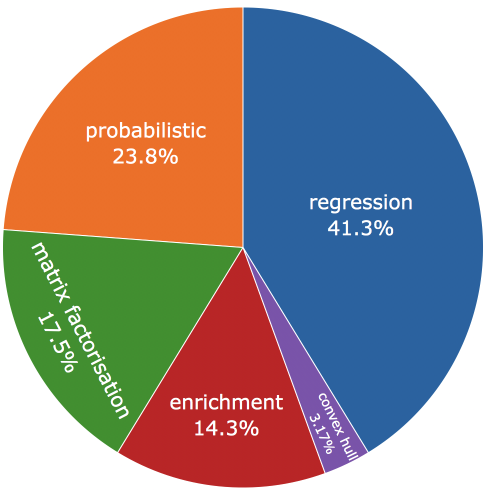
\includegraphics[width=0.33\linewidth]{./figures-ext/piechartA} }\subfloat[supervised/unsupervised\label{fig:languages2}]{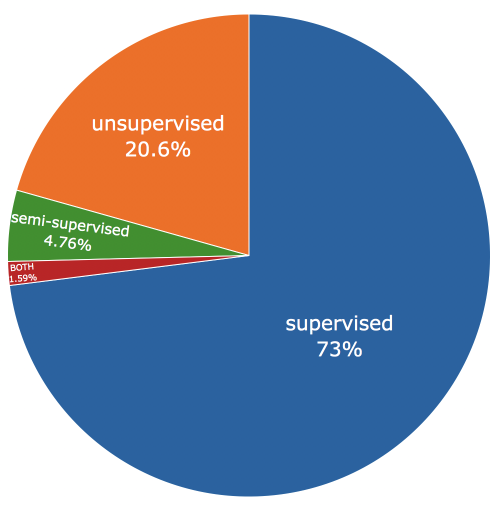
\includegraphics[width=0.33\linewidth]{./figures-ext/pichartB} }\subfloat[programming language\label{fig:languages3}]{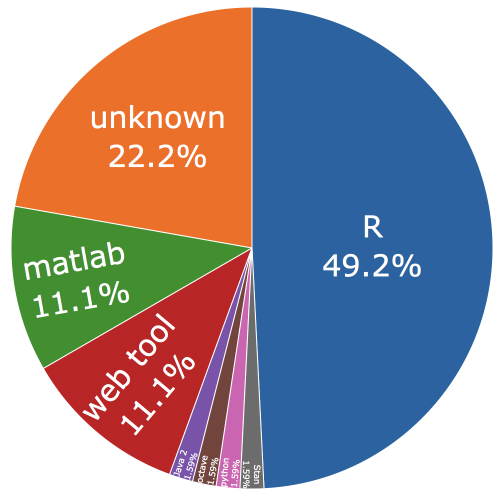
\includegraphics[width=0.33\linewidth]{./figures-ext/pirChart} }\caption[Simple statistics illustrating characteristics of published cell-type deconvolution tools]{\textbf{Simple statistics illustrating
characteristics of published cell-type deconvolution tools}:
\ref{fig:languages1} - Percentage of used approach type,
\ref{fig:languages2} - Percentage of supervised/unsupervised tools,
\ref{fig:languages3} - Percentage of the programming languages of
implementation. Data gathered based on pubmed and google scholar search
in May 2018.}\label{fig:languages}
\end{figure}









\hypertarget{regression-based-methods}{%
\subsection{Regression-based methods}\label{regression-based-methods}}

Regression models are the most popular methods for bulk gene expression
deconvolution. They use estimated pure cell profiles as depending
variables (or selected signature genes) that should explain the mixed
profiles choosing best \(\beta\) parameters (\eqref{eq:regLin}) that can
be interpreted as cell proportions.

A standard type of regression is called linear regression. It reflects
linear dependence between independent and dependent variables. The
linear regression was developed in the \emph{precoputer age of
statistics} \citep{Hastie2009}.

In linear regression, we want to predict a real-valued output \(Y\),
given a vector \(X^T = (X_1,X_2,… ,X_p)\). The linear regression model
has the form:

\begin{equation}
f(X) = \beta_0 + \sum_{j=1}^{p} X_j\beta_j \label{eq:regLin}
\end{equation}

Where the \(\beta_j\)s are unknown parameters or coefficients, and
\(X_j\)s are the explaining variables. Given pairs of
(\(x_1\),\(y_1\))\ldots{}(\(x_N\) ,\(y_N\) ), one can estimate
coefficients \(\beta\) with an optimization of an objective function
(also called cost function).

The most popular estimation method is \textbf{least squares}, the
coefficients \(\beta = (\beta_0, \beta_1, ..., \beta_n)\) are computed
to minimize the residual sum of squares (RSS):

\begin{equation}
RSS(\beta) = \sum_{i = 1}^{N}(y_i - f(x_i))^2 = \sum_{i = 1}^{N}(y_i - \beta_0 - \sum_{j=1}^p x_i\beta_j)^2 \label{eq:rss}
\end{equation}

\textbf{Ordinary least squares regression} is using Eq.\eqref{eq:rss} to
compute \(\beta\).

\textbf{Ridge regression} (Equation \eqref{eq:ridge}) adds a regularizer
(called \(L2\) norm) to shrink the coefficients (\(\lambda \geq 1\))
through imposing a penalty on their size.

\begin{equation}
\hat{\beta}^{ridge} = \underset{\beta}{\text{argmin}}\{\sum_{i = 1}^{N}(y_i - f(x_i))^2 + \lambda\sum_{j=1}^{p}\beta^2_j\}\label{eq:ridge}
\end{equation}

Similarly \textbf{Lasso regression} (Equation \eqref{eq:lasso}) adds a
regularization term to RSS (called \(L1\) norm), it may set coefficients
to 0 and therefore perform feature selection.

\begin{equation}
\hat{\beta}^{ridge} = \underset{\beta}{\text{argmin}}\{\sum_{i = 1}^{N}(y_i - f(x_i))^2 + \lambda\sum_{j=1}^{p}\lvert\beta_j\rvert\}\label{eq:lasso}
\end{equation}

In \textbf{Elastic net regression} both penalties are applied.

\textbf{Support Vector Regression (SVR)} is regression using
\textbf{Supported Vector Machines (SVM)}. In SVR \(\beta\) can be
estimated as follows:

\begin{equation}
H(\beta,\beta_0) = \sum_{i=1}^{N} V (y_i − f(x_i)) +\frac{λ}2\lVert\beta\rVert^2 \label{eq:svr1}
\end{equation}

where error is measured as follows:

\begin{equation}
V_\epsilon(r) = \begin{cases}
    0, & \text{if $\lvert r \rvert < \epsilon$,}\\
    \rvert r\lvert - \epsilon, & \text{otherwise}. 
  \end{cases}  \label{eq:svr2}
\end{equation}

with \(\epsilon\) being the the limit of error measure, meaning errors
of size less than \(\epsilon\) are ignored.

In the SVM vocabulary, a subset of the input data that determine
hyperplane boundaries are called the \textbf{support vectors}
(Fig.\ref{fig:svr}). SVR discovers a hyperplane that fits maximal
possible number of points within a constant distance, \(\epsilon\), thus
performing a regression.

In brief, in SVR, RSS is replaced by a linear \(\epsilon\)-insensitive
loss function and uses \emph{L}2-norm penalty function. There exist
variants of SVR algorithm, i.e. \(\epsilon\)-SVR \citep{drucker1997} and
\(\nu\)-SVR \citep{Scholkopf2000}. \(\epsilon\)-SVR allows to control
the error, this favorizes more complex models. In the \(\nu\)-SVR the
distance of the \(\epsilon\) margin can be controlled and therefore
number of data points used for regression can be controlled.
\citet{Ju2013} used SVM-based method to define cell type specific genes.
A model using \(\nu\)-SVR with linear kernel was used by
\citet{Newman2015} in CIBERSORT.

\begin{figure}

{\centering 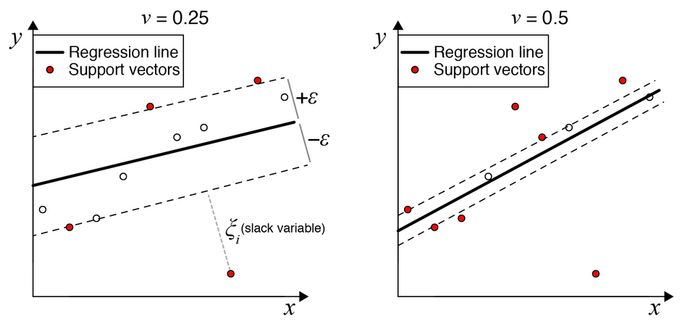
\includegraphics[width=1\linewidth]{figures-ext/vSVR} 

}

\caption[Priciple of the SVR regression]{\textbf{Priciple of the SVR regression}. In SVR
regression \(\epsilon\) represents limit of error measure, input data
points higher than \(+\epsilon\) or lower than \(-\epsilon\) are called
support vectors. The \(\nu\) parameter in \(\nu\)-SVR regression
controls the distance of training error bonds: left - lower \(\nu\)
value larger bound, right - higher \(v\) margin, smaller bound.
Reprinted by permission from Springer Nature \citep{Newman2015} © 2018
Macmillan Publishers Limited, part of Springer Nature. All rights
reserved.}\label{fig:svr}
\end{figure}











As unconstrained optimization of the objective function can result in
negative coefficients. In the context of cell-type deconvolution,
authors often aim to avoid as it complicates the interpretation.
Therefore, different constraints can be imposed to the \(\beta\)
coefficients. The most common conditions are
\(\beta_0 +\beta_1+ ...+\beta_n =1\) and \(\forall\beta_i \geq 0\).
Solution respecting the non-negativity condition is also called
non-negative least squares (NNLS) to contrast with ordinary least
squares (OLS). NNLS was adapted by many authors
\citep{Venet2001, Abbas2009, Repsilber2010, Zuckerman2013, Wang2016}.

The task can be also solved differently from computational perspective.
\citet{Lu2003} and \citet{Wang2006} propose to use simulated annealing
to minimize the cost function. \citet{Gong2011} proposed to solve task
using quadratic programming.

An extensive review on optimisation of the objective function for
regression methods in cell-type deconvolution was published by
\citet{Mohammadi2017}. Authors carefully consider different
possibilities of parameter choice in the loss and regularization
fomulations and its performance. They present as well recommendations
for construction of basis matrix and data pre- and post-processing.
Digital tissue deconvolution (DTD) \citep{Gortler2018} aims to train the
loss function with \emph{in silico} mixtures of single cell profiles
resulting in improved performance of rare cell types (present in small
proportion). However, the training is computationally heavy and the
proper training data for bulk transcriptomes are not available.

Since the publication of CIBERSORT \citep{Newman2015} some authors
\citep{Chen2018, Schelker2017} used the \citet{Newman2015}
implementation directly with pre/post modifications or different
signature matrix or re-implemented the SVR regression \citep{Chen2018}.

Another recent method EPIC \citep{Racle2017} introduced weights related
to gene variability. In their constrained regression, they add it
explicitly in the cost function modifying RSS (Eq.\eqref{eq:rss}):

\begin{equation}
RSS^{weighted} (\beta) = \sum_{i = 1}^{N}(y_i - \beta_0 - w_i \sum_{j=1}^p x_i\beta_j)^2  \label{eq:epic}
\end{equation}

with the negativity and sum constraints we discussed above. The \(w_i\)
weights are corresponding to variance of the given gene measure in the
same cell type. It aims to give less importance to the variant genes.
EPIC also allows a cell type that is not a referenced in the signature
matrix with an assumption that the non-referenced cell type is equal to
1- sum of proportions of other cell types (Eq.\eqref{eq:tumorcoeff}). This
non-referenced cell type is interpreted by authors as the tumor
fraction:

\begin{equation}
\beta_m = 1 - \sum_{j=1}^{m-1}\beta_j \label{eq:tumorcoeff}
\end{equation}

An additional feature of EPIC is advanced data normalisation and an
estimation of mRNA produced by each cell to adjust cell proportions,
which was previously proposed by \citet{Liebner2013} in the context of
microarray data:

\begin{equation}
p_j=\alpha \frac{\beta_j}{r_j} \label{eq:norm}
\end{equation}

where \(p_j\) are actual cell proportions that are `normalized' with
empirically derived coefficient \(\alpha\) and measured \(r_j\) is the
amount of RNA nucleotides in cell type~\(j\).

Recently CIBERSORT proposed an \emph{absolute mode} where the
proportions are not relative to the leucocyte infiltration but to the
sample. It can be obtained with assumption that the estimation of
proportion of all genes in CIBERSORT matrix is corresponding to sample
purity. This functionality was not yet officially published and it is
still in experimental phase \citep{Newman}.

Regression methods combined with pre- and post-processing of data can
result in estimation of proportions that can be interpreted directly as
a percentage of cells in mixed sample. It is an important feature hard
to achieve with other methods. Some methods provide relative proportions
of the immune infiltrate \citep{Newman2015} and other aim to provide
absolute abundance \citep{Racle2017}. The absolute proportions are
easily comparable between data sets and cell types. Regression based
methods are usually quite fast and can process big transcriptomic
cohorts. However, as I will discuss in
\protect\hyperlink{Validation}{Validation} section, they pose on the
hypothesis that the reference profiles available in some context
(i.e.~blood) are valid in a different one (i.e.~tumor) or that profiles
extracted from one data type (scRNA-seq) are adapted to deconvolute bulk
RNAseq. Most of recent regression methods focused on estimating
proportions and do not estimate context specific profiles and can
process as little as one sample.

\hypertarget{enrichment-based-methods}{%
\subsection{Enrichment-based methods}\label{enrichment-based-methods}}

\rowcolors{2}{gray!6}{white}\begin{table}

\caption[Contangency table]{\label{tab:contangency}\textbf{Contangency table} is the count of overlap of
genes present in a certain codition (Y) vs not present (Y-Z) and
association to a pathway X (in X or not in X). Contangency table is used
in frequency based test as Fisher exact test.}
\centering
\begin{tabular}[t]{|>{}l|>{}c|c}
\hiderowcolors
\toprule
\rowcolor{Gray}  \textcolor{white}{\textbf{ }} & \textcolor{white}{\textbf{Y}} & \textcolor{white}{\textbf{Z-Y}}\\
\midrule
\showrowcolors
in X & a & b\\
not in X & c & d\\
\bottomrule
\end{tabular}
\end{table}\rowcolors{2}{white}{white}






Enrichment-based methods aim to evaluate an amount of activity of a
given list of genes within the data. This can be obtained though
calculating a score based on gene expression. Traditionally enrichment
methods were used to analyse set of DEG. Different statistical
approaches were adapted: like fisher exact test giving a p-value that
estimated the chance a given list of genes is over/under present in the
input list of DEGs and therefore characterise the condition vs.~control
expressed genes.

Let's take an example, if one wants to compute enrichment in pathway X
of the list of DEG genes Y with total number of tested genes Z, a
contingency table need to be constructed (Tab. \ref{tab:contangency}).

In the Fisher exact test formula (Eq. \eqref{eq:fisher}) the \(a\),
\(b\),\(c\) and \(d\) are the individual frequencies, i.e.~number of
genes in of the 2X2 contingency table, and \(N\) is the total frequency
(\(a + b + c + d\)).

\begin{equation} 
p= \frac{( ( a + b ) ! ( c + d ) ! ( a + c ) ! ( b + d ) ! )}{a ! b ! c ! d ! N ! } \label{eq:fisher}
\end{equation}

Another famous (\textgreater{}14000 citations) algorithm computing such
a score (enrichment score ES) is named gene set enrichment analysis
(GSEA) \citep{Subramanian2005} uses sum-statistics. The list of genes
user wants to test for enrichment is usually ranked by fold change odd
or p-value of DGE analysis.

The high score indicated high activity of genes included in the list.
GSEA can also indicate an anti-activity of correlation. A variant of
GSEA, single sample GSEA (ssGSEA) \citep{Barbie2009} was used by
\citet{Senbabaoglu2016}, \citet{Yoshihara2013} and \citet{Aran2017} to
compute infiltration scores. In the ssGSEA genes are ranked by their
absolute expression. Variance-based variant of GSEA - GSVA
\citep{Hanzelmann2013} was used by \citet{Tamborero2018} in the same
purpose. MCPcounter \citep{Becht2016} uses an arithmetic mean of gene
expression of highly specific signature genes to compute a score.

In this way obtained scores, are not comparable between different cell
types and datasets. Therefore some authors propose normalization
procedures that make the score more comparable. For instance xCell, uses
a platform-specific transformation of enrichment scores. Similarly,
Estimate transforms scores for TCGA though an empirically derived
formula. MCPcounter authors use z-scoring to minimise platform-related
differences. Unfortunately, the normalization is not directly included
in the R package

Even though enrichment methods do not try to fit the linear model and
derived scores are not mathematically conditioned to represent cell
proportions, usually there can be observed a strong linear dependence.
An advantage of the enrichment-based methods is the speed and
possibility to include diverse signatures that can characterise
cell-types and cell-states of different pathways.

\hypertarget{probabilistic-methods}{%
\subsection{Probabilistic methods}\label{probabilistic-methods}}

The probabilistic methods share a common denominator: they aim to
minimise a likelihood function of Baye's theorem:

\begin{equation} 
p(y|\theta) = \frac{p(\theta|y )* p(y)}{p(\theta)} \label{eq:Bayes}
\end{equation}

In Eq.\eqref{eq:Bayes} \(y\) is our data, \(\theta\) a parameter,
\(p(y|\theta)\) \emph{posterior}, \(p(\theta|y )\) \emph{likelihood} and
\(p(\theta)\) \emph{prior}. Prior distribution is what we know about the
data before it was generated and combined with a probability
distribution of the observed data is called posterior distribution. The
likelihood describes how likely it is to observe the data (\(y\)) given
the parameter \(\theta\) (probability of \(y\) given \(\theta\) -
\(p(y|\theta)\)). A parameter is characteristic of a chosen model and a
hyperparameter is a parameter of prior distribution.

In the literature, there are mainly different types of probabilisitic
models, one that assumes some type of distribution of mixed sources
(i.e.~gaussian or poisson), other that learn the distribution parameters
empirically from a training set, another that try find the parameters of
the distribution given the number of given sources. Then in each case,
there are different ways of constructing different priors and posteriors
functions. Among used techniques are Markov Chain Monte Carlo or
Expectation-Maximisation, which themselves can be implemented in
different ways
\citep[\citet{Zaslavsky2017}]{Erkkila2010, Ghosh2004, Lahdesmaki2005, Li2013, Roy2006}.

The probabilistic approaches are the most popular for purity estimation
(2 components models), that seem to be possible to extend to
3-components model \citep{Wang2017}. As far as cell-type decomposition
into a number of cells is concerned, a method published on BioRxiv
\emph{Infino} uses Bayesian inference with a generative model, trained
on cell type pure profiles. Authors claim their method is notably suited
for deep deconvolution that is able to build cell type similarities and
estimate the confidence of the estimated proportions which help to
better interpret the results.

Probabilisitic framework is an attractive approach with solid
statistical bases. It can be suited to many specific cases. The pitfalls
are (1) the need of prior profiles or correct hypothesis on the
distribution parameters (2) reduced performance when applied to high
dimensional datasets due to extensive parameters search.

\hypertarget{convex-hull-based-methods}{%
\subsection{Convex-hull based methods}\label{convex-hull-based-methods}}

An emerging family of BSS methods are convex geometry (CG)-based
methods. Here, the \emph{sources} are found by searching the facets of
the convex hull spanned by the mapped observations solving a classical
convex optimization problem \citep{Yang2015}. It can be implemented in
many ways \citep{Preparata1985}.

\textbf{Convex hull} can be defined as follows \citep{Erickson2018}:

\begin{quote}
\emph{We are given a set \(P\) of \(n\) points in the plane. We want to
compute something called the \textbf{convex hull} of \(P\). Intuitively,
the convex hull is what you get by driving a nail into the plane at each
point and then wrapping a piece of string around the nails. More
formally, the convex hull is the smallest convex polygon containing the
points:}
\end{quote}

\begin{quote}
\begin{itemize}
\item
  \emph{\textbf{polygon}}: \emph{A region of the plane bounded by a
  cycle of line segments, called \textbf{edges}, joined end-to-end in a
  cycle. Points where two successive edges meet are called
  \textbf{vertices}.}
\item
  \emph{\textbf{convex}: For any two points \(p\), \(q\) inside the
  polygon, the line segment \(pq\) is completely inside the polygon.}
\item
  \emph{\textbf{smallest}}: \emph{Any convex proper subset of the convex
  hull excludes at least one point in \(P\). This implies that every
  vertex of the convex hull is a point in \(P\).}
\end{itemize}
\end{quote}

\begin{figure}

{\centering 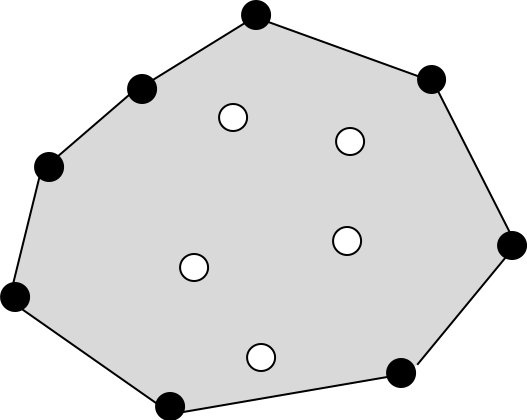
\includegraphics[width=0.5\linewidth]{figures-ext/convexhull} 

}

\caption[Convex hull illustration]{\textbf{Convex hull illustration}. A set of
points and its convex hull (line). Convex hull vertices are black;
interior points are white. Image reproduced after \citet{Erickson2018}.}\label{fig:convexhull}
\end{figure}





Convex hull methods have been used in many fields, from economics and
engineering, I will discuss it with a focus on biological context to
link tightly to cell-type deconvolution.

The main assumptions of Convex hull optimization are that the gene
expression of pure cell types is non-negative and that cell type
proportions are linearly independent.

The shapes can be fitted to a cloud of points in many ways in order to
respond to a given optimality criteria. A popular method introduced by
\citet{Shoval2012} and applied to gene expression and morphological
phenotypes of biological species employ the \textbf{Pareto front}
concept which aims to find a set of designs that are the best trade-offs
between different requirements.

Visually Pareto front correspond to the edge of the convex hull.

\citet{Wang2013} proposed Complex Analysis of Mixtures (CAM) method to
find the Pareto front (the vertices of \(X\) mixed matrix (a convex
set)). In the context of the cell-type deconvolution it can be said that
``the scatter simplex of pure subpopulation expressions is compressed
and rotated to form the scatter simplex of mixed expressions whose
vertices coincide with cell proportions''\citep{Wang2016}. In respect to
the assumptions, under a noise-free scenario, novel \emph{marker genes}
can be blindly identified by locating the~\emph{vertices}~of the mixed
expression scatter simplex \citep{Wang2010}. In the figure (Fig.
\ref{fig:cam}), the \(a_i\)'s are cell-type proportions of \(k\) cell
types, \(s_i\) pure cell type expression and \(x_j\) mixed expression in
sample \(j\). Therefore the vertices correspond to the column vectors of
the matrix \(A\) (Eq. \eqref{eq:linear}). The genes placed in a distance
\(d\) from the vertices can be interpreted as marker genes.

\begin{figure}

{\centering 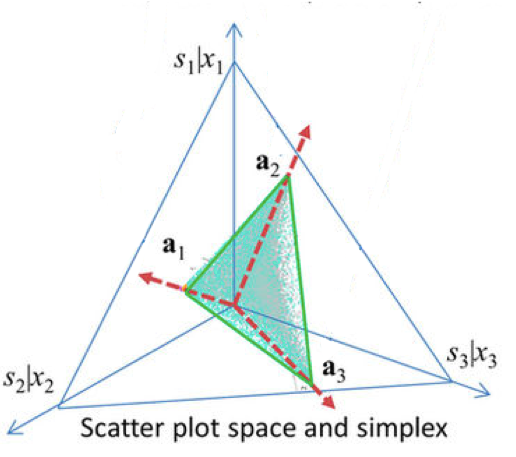
\includegraphics[width=0.5\linewidth]{figures-ext/cam} 

}

\caption[Fitting gene expression data of mixed populations to a convex hull shape]{\textbf{Fitting gene expression data of mixed
populations to a convex hull shape}. Geometry of the mixing operation in
scatter space that produces a compressed and rotated scatter simplex
whose vertices host subpopulation-specific marker genes and correspond
to mixing proportions.}\label{fig:cam}
\end{figure}







In the procedure suggested by \citet{Wang2013}, before performing CAM,
clustering (more precisely affinity propagation clustering (APC) ) is
applied to the matrix in order to select genes representing clusters,
called cluster centers \(g_m\) and dimention reduction(PCA) is applied
to the sample space. Then in order to fit a convex set, a
margin-of-error should be minimized. The Eq. \eqref{eq:camErr} explains
the computation of the error which computes \(L2\) norm of the
difference between \(g_m\) possible vertices and remaining exterior
clusters. All possibilities of combinations drew from \(C^M_K\), \(M\)
number of clusters and \(K\) true vertices, are tested.

\begin{equation}
\begin{aligned}
\text{given }\alpha_k \geq 0, \sum^K_{k=1}\alpha_k=1 \\
\delta_{m, \{1,...,K\} \in C^M_K }= \underset{\alpha_k}{min} \sqrt{{g_m} - \sum^K_{k=1}\alpha_kg_k} \label{eq:camErr}
\end{aligned}
\end{equation}

Once optimal configuration is found, the proportions are computed using
standardised averaging: \begin{equation}
\hat{\alpha_k} = \frac{1}{n_{markers}} \sum_{i \in markers} \frac {x(i)}{\rVert x(i)\lVert}
\end{equation} where \(\hat{\alpha_k}\) is proportion of cell type
\(k\), \(n_{markers}\) number of marker genes (obtained from CAM), and
\(\rVert x(i)\lVert\) is the \(L1\) or \(L2\) norm of a given marker
gene \(x_i\).

Then the cell-type specific profiles are obtained with linear
regression. Authors of CAM also propose a minimum description length
(MDL) index that determines number of sources in the mixture. It selects
the \(K\) minimizing the total description code length.

So far, the published R-Java package \emph{CAM} does not allow to
extract gene specific signatures and it is not scalable to big cohorts
(many samples). In the article, authors apply important pre-processing
steps that are not trivial to reproduce and which are not included in
their tool. Authors apply CAM and validate on rather simple mixtures
(tissue \emph{in vitro} mixtures and yeast cell cycle).

A slightly different approach was proposed by \citet{Newberg2018}. It
does not require initial dimension reduction steps or clustering before
fitting the convex hull and it is based on a probabilisitic framework.
The toll \emph{CellDistinguisher} was inspired by topic modelling
algorithm \citep{Arora2013}. It first computes \(Q\) matrix (Eq.
\eqref{eq:q}). Then each row vector of \(Q\) is normalized to 1 giving
\(\overline{Q}\) matrix. Every row of \(\overline{Q}\) lies in the
convex hull of the rows indexed by the cell-type specific genes. Then
\(L_2\) norm of each row is computes. Genes which rows have the highest
norm can be used as \emph{distinguishers} or \emph{marker} genes. Then
another runs of selections are applied after recentering the matrix to
find more markers.

\begin{equation}
Q=XX^T \label{eq:q}
\end{equation}

Once the set of possible distinguishers is defined, proportions and cell
profiles are computed using Bayesian framework to fit the convex hull.
Authors provide a
\href{https://github.com/GeneralElectric/CellDistinguisher}{user-friendly
R package \emph{CellDistinguisher}}. Unfortunately, they do not provide
any method for estimation of number of sources, which is critical for
source separation of complex tissues. Additionally, quantitative weights
are provided only for signature genes which number can vary for
different sources, and can be as small as one gene. Authors do not apply
their algorithm to complex mixtures as tumor transcriptome, they
establish a proof of concept with \emph{in vitro} mixtures of tissues.

The convex hull-based method does not require the independence of cell
types assumption, nor the non-correlation assumption which can be
interesting in the setup of closely related cell types. In theory, they
also allow \(k>j\) (more sources than samples). So far, the existing
tools are not directly applicable to tumor transcriptomes.

\hypertarget{matrix-factorisation-methods}{%
\subsection{Matrix factorisation
methods}\label{matrix-factorisation-methods}}

Matrix factorisation is a general problem not specific to cell types
deconvolution. It has been extensively used for signal processing
\citep{Zinovyev2013}and extraction of features from images
\citep{Hastie2009}. Matrix factorisation can also be called BSS or
dimension reduction. Despite quite simple statistical bases they have
been proven to be able to solve quite complex problems. Many matrix
factorisation methods can solve the problem of Eq. \eqref{eq:linear}. They
can solve it in different ways and in respect with different hypotheses.

Naturally matrix factorisation methods estimate simultaneously \(A\) and
\(S\) matrices (cell proportions and profiles) given \(X\) rectangualr
matrix (genes \(\times\) samples) without any additional input.

\begin{figure}

{\centering 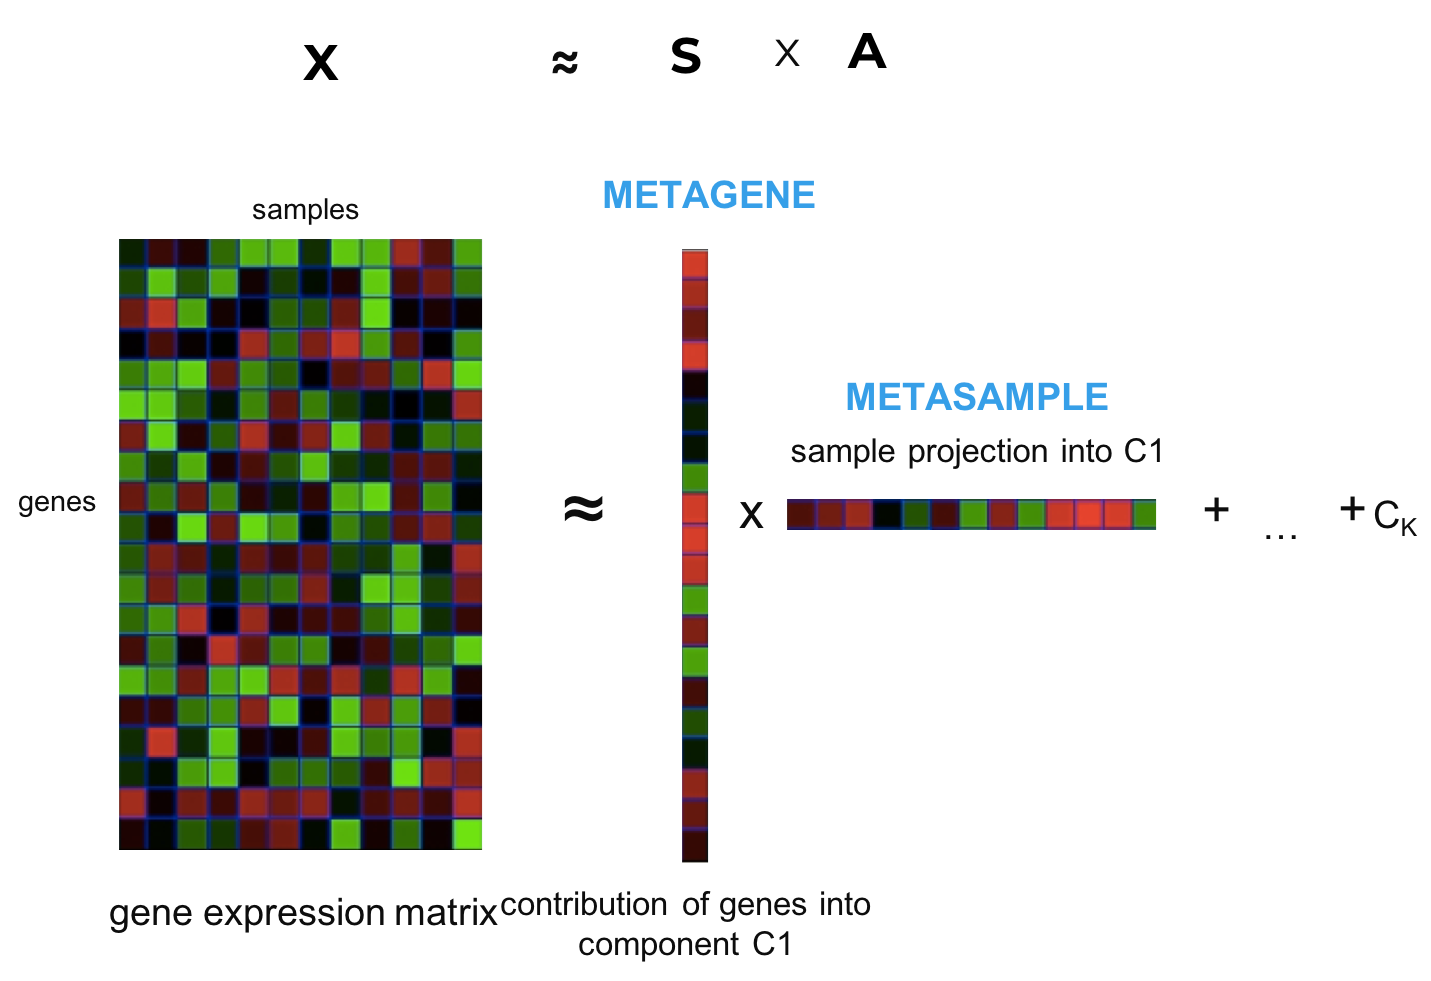
\includegraphics[width=0.8\linewidth]{figures-ext/factor} 

}

\caption[Principle of matrix factorisation of gene expression]{\textbf{Principle of matrix factorisation of gene
expression}. The gene expression matrix \(X\) is decomposed into a set
of \emph{metagenes} \(S\) matrix and \emph{metasamples} \(A\). Number of
components \emph{C} is defined with parametre \(k\).}\label{fig:fact}
\end{figure}






\hypertarget{principal-components-analysis}{%
\subsubsection{Principal Components
Analysis}\label{principal-components-analysis}}

One of the most popular methods, \textbf{Principal Components Analysis}
(PCA). computes projections of the data, mutually uncorrelated and
ordered in variance. The principal components provide a sequence of best
linear approximations to that data.

Traditionally PCA is computed through eigen decomposition of the
covariance matrix. Covariance matrix is computed as follows:

\begin{equation}
\Sigma = \frac{1}{n-1}((X-\bar{x})^T(X-\bar{x})) \label{eq:covPCA}
\end{equation}

where \(\bar{x}\) is mean vector of feature column in the data \(X\).

Then the matrix is decomposed to eigenvalues: \begin{equation}
\mathbf{V^{-1}\Sigma V=D} \label{eq:eigenvecPCA}
\end{equation}

where \(\mathbf{V}\) is matrix of eigenvectors and \(\mathbf{D}\)
diagonal matrix of eigenvalues.

It can be also computed using \textbf{singular value decomposition}
(SVD) (computationally more efficient way):

\begin{equation}
X= UDV^T \label{eq:svd}
\end{equation}

Here \(U\) is an \(N \times p\) orthogonal matrix (\(U^T U = I_p\))
whose columns \(u_j\) are called the left singular vectors; \(V\) is a
\(p \times p\) orthogonal matrix (\(V^T V = I_p\)) with columns \(v_j\)
called the right singular vectors, and \(D\) is a \(p \times p\)
diagonal matrix, with diagonal elements
\(d_1 \geq d_2 \geq ... \geq d_p \geq 0\) known as the singular values.
The columns of \(UD\) are called the principal components of \(X\).

PCA \emph{sees'} the data as a cloud of points and finds directions in
which the samples to define Principal Components. This dispersion is
measured with variance, and resulting PCA components are
variance-ordered.

As nicely described in \citep{Rutledge2013}

\begin{quote}
\emph{The first PC is the vector describing the direction of maximum
sample dispersion. Each following PC describes the maximal remaining
variability, with the additional constraint that it must be orthogonal
to all the earlier PCs to avoid it containing any of the information
already extracted from the data matrix. In other words, each PC extracts
as much remaining variance from the data as possible. The calculated PCs
are weighted sums of the original variables, the weights being elements
of a so-called loadings vector. Inspection of these loadings vectors may
help determine which original variables contribute most to this PC
direction. However, PCs being mathematical constructs describing the
directions of greatest dispersion of the samples, there is no reason for
the loadings vectors to correspond to underlying signals in the data
set. Most of the time, PCs are combinations of pure source signals, and
do not describe physical reality. For this reason their interpretation
can be fraught with danger.}
\end{quote}

Especially in the context of the cell-type deconvolution, it can be
imagine that different cell-types contribute to the variance but one PC
could explain joint variance of many cell types.

\citet{Wang2015} used SVD to compute matrix inversion in order to
separate tumor from the stroma. The method was applied to tumor
transcriptomes and gives purity estimation quite different from other
popular enrichment-based method ESTIMATE \citep{Yoshihara2013}.

\citet{Nelms2016} in CellMapper uses a semi-supervised approach based on
SVD decomposition to dissect human brain bulk transcriptome. Authors
define a query gene (a specific known gene) and then they decompose
transcriptome into components (eigenvectors) and multiply by weights
that are higher for the components correlated with the query gene. Then
the matrix is transformed back to gene \(\times\) samples matrix but
query signal is amplified. The point being to find marker genes that
characterise the same cell-type as the query gene. Authors did not aim
the identification of cell-type proportions or cell types profiles but
identification of cell-type specific markers. They underline
applicability of the method to rare cell types where many markers are
not available. This approach was proposed by authors to be used in order
to prioritize candidate genes in disease susceptibility loci identified
by GWAS.

\hypertarget{non-negative-matrix-factorisation}{%
\subsubsection{Non-negative matrix
factorisation}\label{non-negative-matrix-factorisation}}

Non-negative matrix factorization \citep{Seung1999} is an alternative
approach to principal components analysis. It assumes that data and
components are non-negative. It finds its application in image analysis
and gene expression analysis where data are indeed non-negative. The
\(N \times p\) data matrix \(X\) is approximated by

\[X \approx WH \]

where \(W\) is \(N \times r\) and \(H\) is \(r \times p\),
\(r ≤ max(N,p)\). We assume that \(x_{ij}\) ,\(w_{ik}\),
\(h_{kj}\)\(\geq 0\).

Which is a special case of Eq. \eqref{eq:linear}.

The matrices \(W\) and \(H\) are found by maximizing \begin{equation}
\mathcal{L}(W, H) = \sum^N_{i=1}\sum^{p}_{j=1}[x_{ij} log(WH)_{ij} − (WH)_{ij} ] \label{eq:nmf}
\end{equation}

This is the log-likelihood from a model in which \(x_{ij}\) has a
Poisson distribution with mean \((WH)_{ij}\).

This formula can be maximized through minimization of divergence:

\begin{equation}
\underset{W,H}{min} f(W,H)  = \frac{1}{2}\rVert X-WH\rVert^2_F \label{eq:divNMF}
\end{equation}

Where \(\rVert .\rVert_F\) is Forbenius norm, which can be replaced by
Kullback-Leibler divergence.

The optimization can be done employing different methods:

\begin{itemize}
\tightlist
\item
  \textbf{euclidean} update with multiplicative update rules, it is the
  classic NMF \citep{Seung1999}
  \begin{equation}\begin{aligned} W \leftarrow W \frac{XH^T}{WHH^T}\\H \leftarrow H\frac{W^TX}{W^TWH}  \label{eq:euclidNMF} \end{aligned}\end{equation}
\item
  \textbf{alternating least squares} \citep{Paatero1994} where the
  matrices W and H are fixed alternatively
\item
  \textbf{alternating non-negative least squares} using projected
  gradients (\citet{Lin2007})
\item
  \textbf{convex-NMF }\citep{Ding2010} imposes a constraint that the
  columns of \(W\) must lie within the column space of~\(X\),
  i.e.~\(W = XA\)~(where~\(A\)~is an auxiliary adaptative weight matrix
  that fully determines~\(W\)), so that \(X=XAH\).~In this method only
  \(H\) must be non-negative.
\end{itemize}

The NMF algorithms can differ in initialization method as well and even
in situations where \(X = WH\) holds exactly, the decomposition may not
be unique. This implies that the solution found by NMF depends on the
starting values. The performance of different combinations applied to
MRS data from human brain tumours can be found in
\citet{OrtegaMartorell2012}.

\citet{Brunet2004} created a NMF matlab toolbox and demonstrated
applicability of NMF (using Kullback-Leibler divergence and euclidean
multiplicative update \citep{Lee2000} to cancer transcriptomes with
focus on cancer subtyping (focusing on \(H\) matrix). \citet{Brunet2004}
also proposed a way to evaluate optimal number of factors (sources) to
which matrix should be decomposed.

NMF as imposing non-negaivity in the context of decomposition of
transcriptomes seems as an attractive concepts as both cell profiles and
cell proportions should be non-negative. It is not suprising then that
some authors used NMF to perform cell-type deconvolution.

To my knowledge, \emph{deconf} \citep{Repsilber2010} was the first tool
proposing NMF cell-type deconvolution of PBMC transcriptome, of
considerable dimensions, 80 samples (40 control and 40 case) of
Tuberculosis. \citet{Repsilber2010} employed random initialization and
alternating non-negative least squares to minimize the model divergence.
The complete deconvolution of the transcriptome was used to perform DEG
analysis on the deconvoluted profiles.

\citet{Shen-Orr2013}, not only presented exhaustive literature review
through implementing cell-type deconvolution methods in a R package
\emph{CellMix} \citep{Gaujoux2013} but also proposed a semi-supervised
NMF for cell-type deconvolution and published an R package implementing
different NMF methods \citep{Gaujoux2010}. The semi-supervised version
of NMF proposed by \citet{Gaujoux2013}, need a set of specific marker
genes for each desired cell type. Then at initialization and after each
iteration of the chosen NMF algorithm (applies to some versions of NMF
\citep{Seung1999, Brunet2004, PascualMontano2006}, ``each cell type
signature has the values corresponding to markers of other cell types
set to zero. The values for its own markers are left free to be updated
by the algorithm's own iterative schema''. Applying their algorithm to
\emph{in vitro} controlled dataset {[}GSE11058 \citep{Abbas2009},
testing selected NMF implementations and varying number of markers per
cell, authors observed the best performance with guided version of
\emph{brunet} \citep{Brunet2004} implementation.

\citet{Moffitt2015} applied NMF to separate tumor from stroma in
pancreatic ductal carcinoma (PDAC) using multiplicative update NMF. They
scaled \(H\) matrix rows to 1 so that the values correspond to the
proportions. Authors tested different possibilities of number of sources
(\(k\)), the final number of factors was defined through hierarchical
clustering on gene-by-gene consensus matrix of top 50 genes of each
component.

Finally \citet{Liu2017} proposed post-modified NMF in order to separate
\emph{in vitro} mixtures of different tissues.

In brief, NMF is a popular, in biology, algorithm performing source
separation with non-negativity constraint. It was applied to \emph{in
vitro} cell-mixtures and blood transcriptome showing satisfying accuracy
of cell-type \emph{in silico} dissection and evaluating proportions. It
was also applied in cancer context, however it did not recover cell-type
specific signals but rather groups of signals that could be associated
to cancer or stroma.

\hypertarget{independent-components-analysis}{%
\subsubsection{Independent Components
Analysis}\label{independent-components-analysis}}

Independent Components Analysis is written as in Eq. \eqref{eq:linear}
with assumption that columns of \(S\): \(S_i\) are \emph{independent}
and \emph{non-Gaussian}, which adds orthogonality condition to \(A\),
since \(S\) also has covariance \(I\). It was first formulated by
\citet{Herault1986}

The independence can be measured with entropy, kurtosis, mutual
information or negentropy measure \(J(Y_j )\) \citep{Hyvarinen2000}
defined by

\begin{equation}
J(Y_j ) = H(Z_j ) − H(Y_j ) \label{eq:negentropy}
\end{equation}

where \(Z_j\) is a Gaussian random variable with the same variance as
\(Y_j\) . Negentropy is non-negative, and measures the deviation of
\(Y_j\) from Gaussianity. It is used in a popular implementation of
\textbf{FastICA} \citep{Hyvarinen2000}. Other existing implementations
of ICA are

\begin{itemize}
\tightlist
\item
  Infomax \citep{Bell1995} using Information-Maximization that maximizes
  the joint entropy
\item
  JADE (\citet{Cardoso1993}) on the construction of a fourth-order
  cumulants array from the data
\end{itemize}

However, they are usually a lot slower which limits their application to
big corpus of data and \citet{Teschendorff2007} demntrated that
\emph{FastICA} gives the most interpretable results.

Therefore, I will focus on FastICA implementation as it will be
extensively used in the \protect\hyperlink{results}{Results} part.

FastICA requires \emph{prewhitening} of the data (centering and
whitening). Centering is removing mean from each row of \(X\) (input
data). Whitening is a linear transformation that columns are not
correlated and have variance equal to 1.

\textbf{Prewhitenning }

\begin{enumerate}
\def\labelenumi{\arabic{enumi}.}
\tightlist
\item
  Data centering \begin{equation}
    x_{ij} \leftarrow x_{ij} - {\frac {1}{M}}\sum_{j^{\prime }}x_{ij^{\prime }}  \label{eq:cent}
    \end{equation} \(x_{ij}\): data point
\item
  Whitenning \begin{equation}
   \mathbf {X} \leftarrow \mathbf {E}\mathbf {D} ^{-\frac{1}{2}}\mathbf {E} ^{T}\mathbf {X} \label{eq:whit}
   \end{equation} Where \(\mathbf {X}\) - centered data, \(\mathbf {E}\)
  is the matrix of eigenvectors, \(\mathbf{D}\) is the diagonal matrix
  of eigenvalues
\end{enumerate}

\begin{algorithm}
  \caption{ FastICA multiple component extraction}
  \begin{algorithmic}[1]
  \INPUT{$K $ Number of desired components}
  \INPUT{$X \in \mathbb{R}^{N \times M}$ Prewhitened matrix, where each column represents an $N$-dimensional sample, where $K \leq N$ }
  \OUTPUT{$A \in \mathbb{R}^{N \times K}$ Un-mixing matrix where each column projects  $\mathbf {X}$ onto independent component.}
  \OUTPUT{$S \in \mathbb{R}^{K \times M}$ Independent components matrix, with $M$ columns representing a sample with $K$ dimensions.}
  \begin{equation}\label{eq:fasticaMul}\end{equation}
    \For{$p\gets 1, K$}
        \State $\mathbf{w}_{p} \gets$ \emph{Random vector of length} $N$
        \While{$\mathbf{w_{p}}$ \emph{ changes}}
            \State $\mathbf{w}_p \gets \frac{1}{M}Xg(\mathbf{w}_p^TX)^T - \frac{1}{M}g'(\mathbf{w}_p^TX)1w_p$ 
            \State $\mathbf{w}_p \gets \mathbf{w}_p - (\sum_{j=1}^{p-1}\mathbf{w}_p^T\mathbf{w}_j\mathbf{w}_j^T)^T$
            \State $\mathbf{w}_p \gets \frac{\mathbf{w}_p}{\lVert \mathbf{w}_p \rVert}$
        \EndWhile
    \EndFor 
    \State where $\mathbf {1}$  is a column vector of 1's of dimension $M$ 
     \OUTPUT{$A = [\mathbf{w}_1, ..., \mathbf{w}_K]$}
     \OUTPUT{$S = \mathbf{A}^T\mathbf{X}$}

  \end{algorithmic}

\end{algorithm}

However, the results of this algorithm (Alg. 1. \eqref{eq:fasticaMul}) are
not deterministic, as the \(\mathbf{w}_{p}\) initial vector of weights
is generated at random in the iterations of fastICA. If ICA is run
multiple times, one can measure \textbf{stability} of a component.
Stability of an independent component, in terms of varying the initial
starts of the ICA algorithm, is a measure of internal compactness of a
cluster of matched independent components produced in multiple ICA runs
for the same dataset and with the same parameter set but with random
initialization \citep{Himberg2003}.

Icasso procedure can be summarized in a few steps :

\begin{enumerate}
\def\labelenumi{\arabic{enumi}.}
\tightlist
\item
  applying multiple runs of ICA with different initializations
\item
  clustering the resulting components
\item
  defining the final result as cluster centroids
\item
  estimating the compactness of the clusters
\end{enumerate}

In brief, ICA looks for a sequence of orthogonal projections such that
the projected data look as far from Gaussian as possible. ICA starts
from a factor analysis solution, and looks for rotations that lead to
independent components.

So far, ICA was used to deconvolute transcriptomes into biological
functions
\citep{Biton2014, Engreitz2010, Gorban2007, Teschendorff2007, Zinovyev2013}.
However, it have never been used for cell-type deconvolution.

In theory, ICA outputs: \(S\) could be interpreted as sources and \(A\)
as proportions in the cell-type deconvolution context. In practice, the
fact that the ICA allows negative weights of projections, it makes the
interpretation less trivial.

To my knowledge my \protect\hyperlink{DeconICA}{DeconICA} R-package
(that will be described in the results part) is the first method
allowing interpretation of ICA-based signals as cell-type
context-specific signatures and quantify their abundance in
transcriptome.

\begin{figure}

{\centering 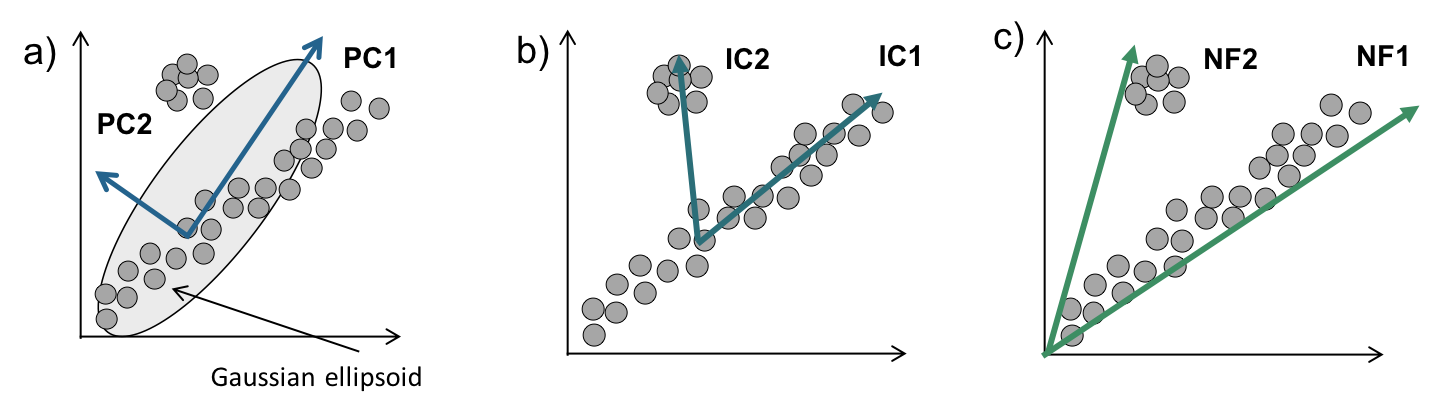
\includegraphics[width=0.8\linewidth]{figures-ext/bss} 

}

\caption[Simple illustration of matrix factorisation methods]{\textbf{Simple illustration of matrix
factorisation methods}. Adapted with permision from \citep{Zinovyev2013}}\label{fig:matrixfact}
\end{figure}




Taken together, matrix factorisation methods are able to decompose a
gene expression matrix into a weigheted set of genes (metagene)(\(S\))
and weigheted set of samples (metasample \(A\)). Discussed here PCA, NMF
and ICA differ in constraints and starting hypotheses. PCA components
are ordered by variance and are orthogonal in the initial space of data
(Fig. \ref{fig:matrixfact} ). NMF impose non-negativy contraint and ICA
independence of sources hypothesis. NMF and ICA do not have a prticular
order. For all the matrix factorization methods number of components (or
factors) (\(k\)) needs to be given to the algorithm. Some authors
propose way to estimate optimal number of components usualy justified in
a specific context. NMF and SVD wera applied in the contex of cell-type
deconvolution while ICA, so far, was used to dissect transcriptome into
factors related to signaling pathwyas, technical biases or clinical
feautres. In addition, ICA was proven to find reproducible signals
between different datasets \citep{Cantini2018, Teschendorff2007}. I am
going to discuss this aspect in the {[}Results{]} section.

\hypertarget{attractor-metagenes}{%
\subsection{Attractor metagenes}\label{attractor-metagenes}}

A method proposed by \citet{Cheng2013}, that can be run in
semi-supervised or unsupervised mode, is called attractor metagenes.
Authors describe their rationale as follows:

\begin{quote}
\emph{We can first define a consensus metagene from the average
expression levels of all genes in the cluster, and rank all the
individual genes in terms of their association (defined numerically by
some form of correlation) with that metagene. We can then replace the
member genes of the cluster with an equal number of the top-ranked
genes. Some of the original genes may naturally remain as members of the
cluster, but some may be replaced, as this process will ``attract'' some
other genes that are more strongly correlated with the cluster. We can
now define a new metagene defined by the average expression levels of
the genes in the newly defined cluster, and re-rank all the individual
genes in terms of their association with that new metagene; and so on.
It is intuitively reasonable to expect that this iterative process will
eventually converge to a cluster that contains precisely the genes that
are most associated with the metagene of the same cluster, so that any
other individual genes will be less strongly associated with the
metagene. We can think of this particular cluster defined by the
convergence of this iterative process as an ``attractor'' i.e., a module
of co-expressed genes to which many other gene sets with close but not
identical membership will converge using the same computational
methodology.}
\end{quote}

Which in pseudocode works as described in Algorithm 2 \eqref{eq:attr} and
it is implemented in R code is available online in
\href{https://www.synapse.org/\#!Synapse:syn1446295}{Synapse portal}.

\begin{algorithm}
  \caption{ Attractor metagenes algorithm}
  \begin{algorithmic}[2]
  \INPUT{$\alpha$ shrinkage parameter}
  \INPUT{$X \in \mathbb{R}^{N \times M}$ gene expression matrix }
  \OUTPUT{$m_j$ metagene of $g_{seed}$ }

    \begin{equation}\label{eq:attr}\end{equation}
    \State{$g_{seed} \gets$ \emph{a gene from} $1:N$ }
    \State{$I^{\alpha}(g_{seed}; g_i)$} \Comment{compute association beteen $g_{seed}$ and $g_i$}
    \State{$w_i = f(I^{\alpha}(g_{seed}; g_i))$} \Comment{compute weights for each gene}
    \State{$m_0 = \frac{\sum^N-1_{i=1}(g_iw_i)}{\sum^N-1_{i=1}w_i} $}\Comment{compute metagene as weighted average of all genes}
    \State{$I^{\alpha}(m_0; g_i)$} \Comment{compute association between metagene $m_0$ and each gene $g_i$}
    \Repeat 
        \State{$w_i = f(I^{\alpha}(m_0; g_i))$}
    \State{$m_j = \frac{\sum^N-1_{i=1}(m_0w_i)}{\sum^N-1_{i=1}w_i} $}
    \Until {$m_{j+1} =  m_j$}

  \end{algorithmic}

\end{algorithm}

The produced signatures' weights are non-negative. In the original
paper, the generation of tumor signatures leads to three reproducible
signatures among different tumor types, including \emph{leucocyte}
metagene. Typically with the essential parmeter \(\alpha=5\), they
discovered typically approximately 50 to 150 resulting attractors.

Attractor Metagenes algorithm can be seen as a variant of clustering
approach where distance metric is mutual information between genes and
metagenes are weighed average of gene expression. This method was
further to study breast cancer \citep{AlEjeh2014} and to SNP data
\citep{Elmas2016}.

There is a possibility to tune the \(\alpha\) parameter in order to
obtain more or less metagenes that would be possibly interpretable as
cell-type signatures.

\hypertarget{others-aspects}{%
\subsection{Others aspects}\label{others-aspects}}

Here I will discuss transversal aspects common to most of deconvolution
methods. They play critical role in the final results and are often
omitted while algorithms are published which impacts significantly the
reproducibility.

\hypertarget{types-of-biological-reference}{%
\subsubsection{Types of biological
reference}\label{types-of-biological-reference}}

Let us consider the most common case of the deconvolution where neither
\(A\) or \(S\) are not known (Eq. \eqref{eq:linear}) and we would like to
estimate cell proportions or both cell proportions and cell profiles. No
matter if the method is supervised or unsupervised at some point of the
protocol the biological knowledge about cell types is necessary in order
to either derive the model or interpret the data. I discussed signatures
from biological perspective in
\protect\hyperlink{immune-signatures}{Section X}. Here, I would like to
stress the importance of the design of gene signatures which aim is to
facilitate cell-type deconvolution.

Depending on chosen solution different type of reference can be used. In
regression algorithms a proxy for purified cell profiles are necessary
to estimate proportions. However, the genes that are the most variant
between cell types are enough for regression and not all profiles are
necessary. The choice of the genes and the number of the genes impacts
significantly the outcome \citep{Vallania2017}. Therefore, most of
regression methods come together with a new \textbf{basis matrix},
ranging from hundreds to tens of genes. Normally, genes selected for
basis matrix should be cell-type specific in respect to other estimated
cell types, validated across many biological conditions
\citep{Hoffmann2006}. \citet{Racle2017} adds a weight directly in the
regression formula (see Eq. \eqref{eq:epic} ) that corresponds to the
variability of a signature gene between independent measurements of the
same cell type so that the least inter-cell type variable genes have
more weight in the model. \emph{CellMix} \citep{Gajoux2013} regroups
different indexes to select the most specific genes based on
signal-to-noise ratio. However, the most popular method is selection of
differentially expressed genes between pure populations. Often criteria
for optimal number of genes in the basis matrix are not knowledge-based
but data-driven. \citet{Abbas2009} uses condition number of basis matrix
(\emph{kappa}) in order to select the number of genes. The same approach
is followed by CIBERSORT and many other regression methods.
\citet{Newman2015} also added another step while constructing the basis
matrix, it preselects reference profiles having maximal discriminatory
power. Some authors \citep{Ju2013, Nelms2016} propose to find marker
genes though correlation with a provided marker gene (a single one or a
group of genes).

In enrichment methods, \textbf{gene list} can be enough to estimate cell
abundance, sometimes (i.e.~GSEA) ranked gene list is necessary. The
choice of extremely specific markers is crucial for accurate call-type
abundance estimation. The choice of markers can also be
platform-dependent, this point is strongly underlined in
\citep{Becht2016}. Interesting possibility is the use of gene list of
different \emph{cell states} in order obtain coarse-grain resolution.

The impact of missing gene from a signature in the bulk dataset remains
an unanswered question. It would be logical that shorter the gene list
for a specific cell, a lack of a gene can have more impact on the
result. There is a need of an accurate threshold between robustness and
accuracy of the method.

In unsupervised methods, purified cell-profiles, signatures or list of
genes can be used \emph{\textbf{a posteriori}} to interpret the obtained
sources. Even though the choice of reference do not affect the original
deconvolution, it affects the interpretation. The advantage of \emph{a
posteriori} interpretation is a possibility to use different sources and
types of signatures in order to provide the post plausible
interpretation. It is common, that the way of interpretation of
components is not included in the deconvolution tool (\citet{Wang2016},
\citet{CellDistinguisher}, \citet{Nanodissection}), even though it is a
crucial part of the analysis.

For the deconvolution of tumoral biopsies, most of reference profiles,
up to now, are coming from the blood, which is the most available
ressource. Therefore most of methods make a hypothesis that blood
cell-type profiles/signatures are correct approximation of cancer
infiltrating immune cells. Rare models like PERT \citep{Qiao2012} or
ImmuneStates \citep{Vallania2017} discuss the perturbation of the
blood-derived profiles in diseases.

With availability of single-cell RNA-seq of human cancers
\citep{Chung2017, Lavin2017, Li2017, Puram2017, Schelker2017, Tirosh2016, Zheng2017},
we gain more knowledge on immune cells in TME and there is a growing
evidence that they differ importantly from blood immune cells.
\citet{Racle2017} show that lymph node resident immune cells have
expression profile closer to blood immune cells than cancer immune
cells. \citet{Schelker2017} shows, using a synthetic bulk dataset, that
using single cell profiles with existing regression methods (CIBERSORT)
can improve their performance in the cancer context. However,
availability of scRNA-seq remains succinct and probably do not embrace
the patient heterogeneity that can be found in big bulk transcriptome
cohorts.

\hypertarget{data-normalization}{%
\subsubsection{Data normalization}\label{data-normalization}}

Data pre- and post-processing can have an important impact on the
deconvolution. Many authors apply stong filetering of genes
\citep{Wang2016}, removing probes with low and moderate expression as
well as genes with the highest expression (potential outliers). In many
cases, data preprocessing is not detailed and therefore impossible to
reproduce.

There is also a debate on the data normalization. Most of authors
suggest to use counts (not log-space) for estimating cell abundance as
log) transformed data violate the libearity assumption
\citep{Zhong2013}, some opt against it \citep{Shannon2010, Clarke2010}
and some envisage both possiblities {[}\citet{Erkkila2010};
\citet{Repsilber2010}). For the RNA-seq data TPM (transcriprs per
milion) normalization is paciced or even required by most methods
(\citet{Chen2018}; \citet{Finotello2017}; \citet{Racle2017}).

\hypertarget{Validation}{%
\subsubsection{Validation}\label{Validation}}

Most of algorithm validation starts with \emph{in silico} mixtures. In
published articles, the bulk transcriptome is simulated in two ways (1)
mixing numerically simulated sources at defined proportions of given
distribution (i.e.~uniform) using linear model (for instance NMF) (2)
using sampling (for instance Monte Carlo) to randomly select existing
pure profiles and mixing them (additive model) at random proportions. To
the obtained bulk samples, noise can be added at different steps of the
simulation. Additional parameters can be defined in \emph{in silico}
mixtures, for instance, CellMix allows defining number of marker genes
(specific to only one source) for each cell type. The simulated
benchmark based on single cell data was used in \citet{Schelker2017} and
\citet{Gortler2018}. In this framework simulated data was obtained
though summing single cell profiles at known proportions. The main
pitfall of those methods is that in the proposed simulations the gene
covariance structure is not preserved. In reality, the proportions of
cell types are usually not random and some immune cell types can be
correlated or anti-correlated. In addition, these simulations create a
simple additive model which perfectly agrees with the linear
deconvolution model. This is probably not the case of the real bulk data
affected by different factors as cell cycle, technical biases, patients
heterogeneity and especially cell-cell interactions.

Naturally, algorithms validated with simulated mixtures are then
validated with controlled \emph{in vitro} mixtures of cell types or
tissues mixed in known proportions. The most popular benchmark datasets
are:

\begin{itemize}
\tightlist
\item
  mix of human cell lines Jurkat, THP-1, IM-9 and Raji in four different
  concentration in triplicates and the pure cell-line profiles
  (\href{https://www.ncbi.nlm.nih.gov/geo/query/acc.cgi?acc=GSE11058}{GSE11058})
  \citep{Abbas2009};
\item
  mix of rat tissues: liver, brain, lung mixed in 11 different
  concentrations in triplicates and the pure tissues
  expression(\href{https://www.ncbi.nlm.nih.gov/geo/query/acc.cgi?acc=GSE19830}{GSE19830})
  \citep{ShenOrr2010}
\end{itemize}

Similar simple mixtures are proposed also by other authors
\citep[\citet{Kuhn2011}]{Becht2016}. This type of benchmark adds
complexity of possible data processing and experimental noise. However,
it still follows an almost perfect additive model as the cell/tissues do
not interact and they are only constituents of the mixture.

Several tools performed systematic benchmark using PBMC or whole blood
datasets, where for a number of patients (that can be over one hundred)
FACS measured proportions of selected cell types and bulk transcriptomes
are available. Many of such datasets can be found at
\href{http://www.immport.org/immport-open/public/home/home}{IMMPORT}
database. \citet{Aran2017} kindly shared with scientific community two
datasets with considerable number of patients (\(\sim80\) and
\(\sim110\)) and processed FACS data (actual proportions) on their
\href{https://github.com/dviraran/xCell/blob/master/Dev_scripts/xCell_ImmPort.zip}{github
repository}. It is still important to remember that liquid tissues are
easier to deconvolute and for the tools using \emph{a priori} reference,
the reference profiles are obtained from the blood. Therefore the
context remains consistent.

Fo the cancer solid tissues deconvolution, some of the tools were
validated with the stained histopathology cuts using in
situ-hybridisation (ISH) \citep{Kuhn2011} or immunohistochemistry (IHC)
(\citet{Becht2016}). Often this method estimate a limited number of cell
types and the measured abundance from pictures can also be biased by the
technical issues (image/ staining quality).

Authors of EPIC validated thier tool with paired RNAseq and Lymph node
FACS-derived proportions in 4 patients
(\href{https://www.ncbi.nlm.nih.gov/geo/query/acc.cgi?acc=GSE93722}{GSE93722}).
They also noticed that it is more straightforward to correctly evaluate
lymph node immune cell types than cancer infiltrating cell types as
lymph node resident cells are more similar to the blood immune cells.

FACS and gene expression of blood cancer (Folicular lymphoma) was also
used by \citet{Newman2015} for a 14 patients (unpublished data). For
solid tissues \citet{Newman2015} used paired FACS and expression
datasets of lung normal tissues for B-cell and CD8 and CD4 T cels of 11
patients (unpublished data).

Some authors proposed to cross validate estimated proportions with
estimated proportions based on a different data input (i.e.~methylome)
\citep[\citet{Senbabaoglu2016}]{Li2016} or CNA
(\citet{Senbabaoglu2016}). This type of validation is interesting, even
though in many projects only one type of data types is available for the
same samples. TCGA data is one of few exceptions.

Finally, a validation of deconvolution of solid cancer tissues remains
incomplete as no paried expression and FACS data is available up to
date.

\hypertarget{statistical-significance}{%
\subsubsection{Statistical
significance}\label{statistical-significance}}

Little number of tools propose a statistical significance assessment.
CIBERSORT computes empirical p-values using Monte Carlo sampling. Infino
authors \citep{Zaslavsky2017} provide a confidence interval for the
proportion estimations. This allows to know which proportion estimation
are more trustful than other.

Most tools compare themselves to others measuring accuracy of the
prediction, or Pearson correlation, on the benchmark datasets (described
above). Often, in the idealized mixtures, methods perform well.
Evaluation of their performance in cancer tissues remains unanswered
without proper statistical evaluation.

\hypertarget{summary-2}{%
\subsection{Summary}\label{summary-2}}

The field of computational transcriptome deconvolution is constantly
growing. Initially used to solve simple in vitro or simulated mixtures
of quite distinct ingredients, then to deconvolute blood expression
data, finally applied to solid cancer tissues. In cancer research
digital quantification of cancer purity become a routine part of big
cancer research projects \citep{Yoshihara2013}. Cell-type
quantification, even though the validation framework and statistical
significance of deconvolution tools can still be improved, seems to be
considered as a popular part of analytical pipeline of bulk tumor
transcriptomes \citep{Cieslik2017}. Different types of approaches try to
solve the deconvolution problem, focusing on different aspects of the
quantification, or proposing methodologically different approaches.
Methods proposing unsupervised solution to the deconvolution problem of
transcriptomes are still underrepresented. All the tools assume a linear
additive model without explicitly including impact of possible
interactions on the cell-type quantification. The tools that met the
biggest success were proven by the authors to be easily applicable to a
variety of cancer datasets and reusable without an extra effort (through
a programming library or web interface). The field is still waiting for
a gold standard validation benchmark that would allow a fair comparison
of all the tools in solid cancer tissues. It is also remarquable that
the recent methods focus on quantification of abundance of average
representation of cell-types without aspiring to deconvolute the
cell-type context-specific profiles. Thanks to diverse cancer single
cell data and big-scale projects \citep{Regev2017}, we will be able to
improve the existing deconvolution approaches and finally replace the
collection of bulk transcriptomes by a collection of scRNA-seq ones.

\hypertarget{otherDecon}{%
\section{Deconvolution of other data types}\label{otherDecon}}

The transcriptome data is not the unique omic data type that can be used
to infer cell type proportions. Genomic and epigenomic data was used in
numerous publications to perform cell-type deconvolution or estimate
sample purity. I will present a general landscape of the tools and
methods used for this purpose.

\hypertarget{dna-methylation-data}{%
\subsection{DNA methylation data}\label{dna-methylation-data}}

Cell-type composition can be computed from DNA methylation data
(described in \protect\hyperlink{epi}{Section X}). In EWAS (Epigenome
Wide Assotication Studies) variation origination from cell types is
considered as important confounding factor that should be removed before
comparing cases and controls and defining Differentialy Methylated
Positions (DMPs). \citet{Teschendorff2017} reviewed 10 tools for
epigenome deconvolution. Six of the described methods are identified by
authors as reference-free (which I called in this Chapter
\emph{unsupervised}), three are regression-based and one is
semi-supervised.

Unsupervised methods employed in methylome cell-type deconvolution are
RefFreeEWAS \citep{Houseman2014}, SVA \citep{Leek2007} are based on SVD,
ISVA based on ICA {[}\citet{Teschendorff2011}) are more general methods
that aim to detect and remove confounders from the data (that do not
need to be necessary the cell types). RUVm \citep{Maksimovic2015} is
semi-supervised method using generalized least squares (GLS) regression
with negative reference also used to remove \emph{unwanted variation}
from the data and could be potentially adapted to cell-type
deconvoltion. EWASher (\citet{Zou2014}) is linear mixed model and PCA
based method that corrects for cell-type composition. Similarly,
ReFACTor \citep{Rahmani2016} use sparse PCA to remove the variation due
to cell-type proportions. \citet{Houseman2016} proposed RefFreeCellMix:
a NMF model with convex constraints to estimate factors representing
cell types and cell-type proportions and a likelihood-based method of
estimating the underlying dimensionality~(\(k\) number of factors). A
different tool MeDeCom \citep{Lutsik2017} uses alternating non-negative
least squares to fit a convex hull.

As far as supervised methods are concerned, EPiDISH
(\emph{E}pigenetic~\emph{D}issection
of~\emph{I}ntra-\emph{S}ample-\emph{H}eterogeneity) R-package
\citep{Teschendorff2017} includes previously published tools: Quadratic
programming method using reference specific DNAse hypersensitive sites
{[}Constrained Projection (CP) \citep{Houseman2012}), adapted to
methylome deconvolution CIBERSORT algorithm (\(\nu\)-SVR) and robust
partial correlations~(RPC) method (a form of linear regression).
Reference cell-type specific profiles were obtained from the blood.

eFORGE \citep{Breeze2016} can detect in a list of DMPs if there is a
significant cell-type effect.

EDec \citep{Onuchic2016} uses DNAm to infer factors proportions using
NMF and then derives factors profiles though linear regression of
transcriptome data of cancer datasets. Authors identify tumor and stroma
compartments and profiles. However, they admit the error rate for
profiles is quite high for most genes.

\citet{Wen2017} focused on intra-tumor heterogeneity (clonal evolution)
based on DNAm data. Profiles obtained from cell lines were used in a
regression model to identify the proportions of sub-clones in breast
cancer data. InfiniumPurify \citep{Zheng2017} and LUMP (\citet{Aran2015}
) uses DNAm to estimate sample purity.

Validation framework for methylation deconvolution is very similar to
transcriptome ones: in silico mixtures and FACS-measured proportions of
the blood. Most of the tools assume the cell composition is a factor the
most contributing to the variability and therefore SVD/PCA based
approaches are sufficient to correct for the variability. According to
\citet{Teschendorff2017} this assumption was not proven to hold true in
solid tissues like cancer. Supervised methods have the same drawback as
in the case of transcriptome, they use purified profiles from one
context to derive cell proportions in a different context. In overall,
it seems that there was no study that proposed cell-type quantification
based on methylome profiles in pan-cancer manner.

\hypertarget{copy-number-aberrations-cna}{%
\subsection{Copy number aberrations
(CNA)}\label{copy-number-aberrations-cna}}

To my knowledge there is no method using CNA data in order to estimate
cell-type composition, as CNA occur in tumor tissue and natural
distinction can be made between tumor and normal cells and within tumor
cells (intra-tumor).

Therefore, copy number aberrations can be used to estimate tumor purity
and clonality. BACOM 2.0 \citep{Fu2015}, ABSOLUTE \citep{Carter2012},
CloneCNA \citep{Yu2016}, PureBayes \citep{Larson2013}, CHAT
\citep{Li2014}, ThetA \citep{Oesper2013}, SciClone \citep{Miller2014},
Canopy \citep{Jiang2016}, PyClone \citep{Roth2014}, EXPANDS
\citep{Andor2014} estimate tumor purity and quantify true copy numbers.
\href{https://omictools.com/tumor-purity-and-heterogeneity-category}{OmicTools
website} reports 70 tools serving this purpose and their review goes
beyond the scope of my work. Most of tools use tumor and normal samples,
paired if possible.
\href{https://github.com/DeveauP/QuantumClone/}{QuantumClone} seem to be
the only tool that requires a few samples from the same tymor (in time
or space dimension).

\citet{Aran2015} published Consensus measurement of purity estimation
that combines purity estimations based on different data types
(available in \href{http://www.cbioportal.org/}{cBioportal}) using:
ESTIMATE \citep{Yoshihara2013} (gene expression data), ABSOLUTE
\citep{Carter2012} (CNA), LUMP \citep{Aran2015} (DNAm and IHC of stained
slides. Authors concluded that the estimation based on different data
types highly correlate with each other, besides the IHC estimates, which
suggests that IHC provides a qualitative estimation of purity.

\hypertarget{summary-of-the-chapter-1}{%
\section{Summary of the chapter}\label{summary-of-the-chapter-1}}

A plethora of machine learning solutions have been developed to solve
problems of different nature. Supervised and Unsupervised approaches can
be distinguished depending if a model is provided set of training data
with known response or the algorithm works blindly trying to find
patterns in the data. Some of the algorithms found an important
application in healthcare and are included in clinical routine.

One of important problems that can, in theory, be solved with ML, is
bulk omic data deconvolution. Different types of deconvoluton of cancer
samples can be distinguished: clonal, purity and cell-type
deconvolution. Here I focused on cell-type deconvolution of
transcriptome data. Through an extensive review I presented 64 tools and
divided them in categories depending on adapted type of approach. I
distinguished probabilistic, enrichment-based, regression-based, convex
hull, matrix factorisation and attractor metagene approaches that can be
used for cell-type deconvolution. I detailed basis of the different
models and highlighted the most important features counting for
cell-type deconvolution.

DNAm data were also used to estimate cell-type proportions. However, the
heterogeneity found in methylome data resulting from difference in cell
type proportions is usually seen as a confounding factor to be removed.
CNA data can be used for estimation of tumor purity and clonality.

In brief, for the transcriptome cell-type deconvolution, it can be
observed that just a limited number of tools are usable in practice in
order to deconvolute big cancer cohorts and without need to provide hard
to estimate parameters. Supervised methods appleid to cancer use
reference-profiles coming from different context. Unsupervised tools, so
far, are rather underrepresented in the field and do not offer a
solution directly applicable to cancer transcriptomes of high
dimensions. All of the presented methods are still waiting for
consistent validation with gold standard benchmark. This could be done
if systematic data of bulk transcriptome paired with FACS-measured
cell-type proportions information for many cell and in many samples were
generated. Another unanswered question is the validity of the linear
mixture model in the presence of cell-cell interactions.

There is still a room for improvement in the field in order to provide
more user-friendly, accurate and precise cell-type abundance
estimations.

A question can be asked, \textbf{are cell-type proportions enough to
understand tumor immune phenotypes?} Can we extract more valuable
information from the bulk omic data that would give use insight to
biological functions of the \emph{in silico} dissected cells?

\hypertarget{objectives}{%
\chapter*{Objectives}\label{objectives}}
\addcontentsline{toc}{chapter}{Objectives}

In the introduction, I have described two sides of studying TME
complexity. I placed in the context of cancer research and cancer
therapy the most recent studies of tumor immunity with focus on
system-level computational approaches. I have also introduced a wide
array of available approaches to address deconvolution of bulk omic
data. I reviewed thier strong and weak points and I presented general
trends since the field was established.

Answers to important questions on \emph{how TME modulates tumor},
\emph{how to propose better cancer subtyping for immune therapies} and
\emph{how to better predict a response to treatment} are perhaps hidden
in already produced bulk omic data. However, new methodological tools
and more overall view is needed to better uncover hidden patterns.

In this thesis I aim to bring new insights into composition and function
of TME. It is clear that complex information is necessary to understand
the role of different immune cells in cancer and not only presence but
also function are to be deciphered from available data. Therefore, this
project, on its biological side, has two main aims:

\begin{enumerate}
\def\labelenumi{\arabic{enumi}.}
\tightlist
\item
  fundamental research: understand presence of different cell type,
  their interactions and functions in TME of different cancers types and
  how other factors as stress, cell cycle etc. shape them. Thanks to
  data-driven and discovery nature of the project, I will also hope to
  understand how signature of cell type evolves in different conditions
  shaped by other cells and factors.
\item
  translational research: how immune landscape and its state can help to
  predict patient survival and better tailor recommendation for therapy.
  The analysis could also bring to the light possible biomarkers or drug
  targets for immune therapies.
\end{enumerate}

I aim to explore publicly available data, challenge inter-lab and
inter-platform biases. I will use mainly bulk transcriptomic data
(because of accessible volume) and cross-validate with other data types:
scRNA-seq, FACS, IHC when possible.

On its computational/mathematical side it will face following
challenges:

\begin{enumerate}
\def\labelenumi{\arabic{enumi}.}
\tightlist
\item
  Establish state-of-art of existing bulk deconvolution methods, discuss
  their advantages and limits
\item
  Propose new unsupervised method that will fill the knowledge gap
  giving an insight into context-specific signatures of cell types/cell
  states in cancer
\item
  Deliver well-documented and user friendly tool that can be used by the
  scientific community
\item
  Decompose a big corpus of bulk omic data into interpretable biological
  functions, with a particular focus on the immune cell types
\item
  Use different data types (scRNAseq, microarray, RNAseq, FACS etc.) to
  complete, compare and contrast findings of the analysis.
\item
  Decompose established immune cells populations from metastatic
  melanoma in order to better understand cell-type heterogeneity
\end{enumerate}

In order to face those challenges, I have first focused on testing and
creating new methods. This is why methods and results are interlaced in
this thesis. Reproducing work of other researchers it is not always
easy, sometimes it is even impossible. A lot of time was invested to
understand and reuse previous publications, part of this effort was
reflected in the introduction, some of my thoughts will be expressed in
the discussion.

Next important step was improving and testing ideas born in our team. I
collaborated to a publication on a topic (Chapter X) and I have authored
an extension of this work described in Chapter Z. I have also compared
my tool to other similar methodn an overview of the results are in
Chapter U.

Once I have found the most appropriate way to apply my method, that I
validated with multiple datasets, I have build a tool to share it with
scientific community. The tool is freely available online as an R
package. During my work, I have collected many datasets of tumor
signatures, tumor metagenes, benchmark datasets some of which are part
of my tool. I have also accessed, thanks to curtesy of our collaborators
a collection of pan-cancer bulk transcriptomic datasets that I competed
with other publicly available datasets. I build my working environment
in which I managed and cleaned the data.

Finally, I realized a pan-cancer analysis of over 100 datasets which is
the main outcome of my work. I completed results of this work with
published scRNAseq data from tumor samples. This analysis is a source of
many information, I have, so far, explored only part of possible
direction focusing on cancer infiltrating T-cells. This results will be
find in a manuscript in preparation in Chapter X. However, more
information can still be extracted in the further work. There is also a
possibility to provide an experimental validation to my finding and it
will be considered in the discussion part.

In parallel, I used part of methods to study cell-type heterogeneity in
an independent project resulted in a submitted publication.

The remaining time, I have invested into collaborations and
contributions to different works within and outside of my team.
Published work from those projects will be shortly described in Annexes.

\hypertarget{part-results}{%
\part{Results}\label{part-results}}

\hypertarget{sens}{%
\chapter{Study of sensitivity and reproducibility of known
methods}\label{sens}}

\hypertarget{finding-optimal-number-of-components-and-over-decomposition-of-transcriptopmes}{%
\section{Finding optimal number of components and over-decomposition of
transcriptopmes}\label{finding-optimal-number-of-components-and-over-decomposition-of-transcriptopmes}}

\begin{itemize}
\tightlist
\item
  Explain why this problem is important
\item
  Explain shortly my role in the paper
\end{itemize}

\citep{Ulykbek2017}

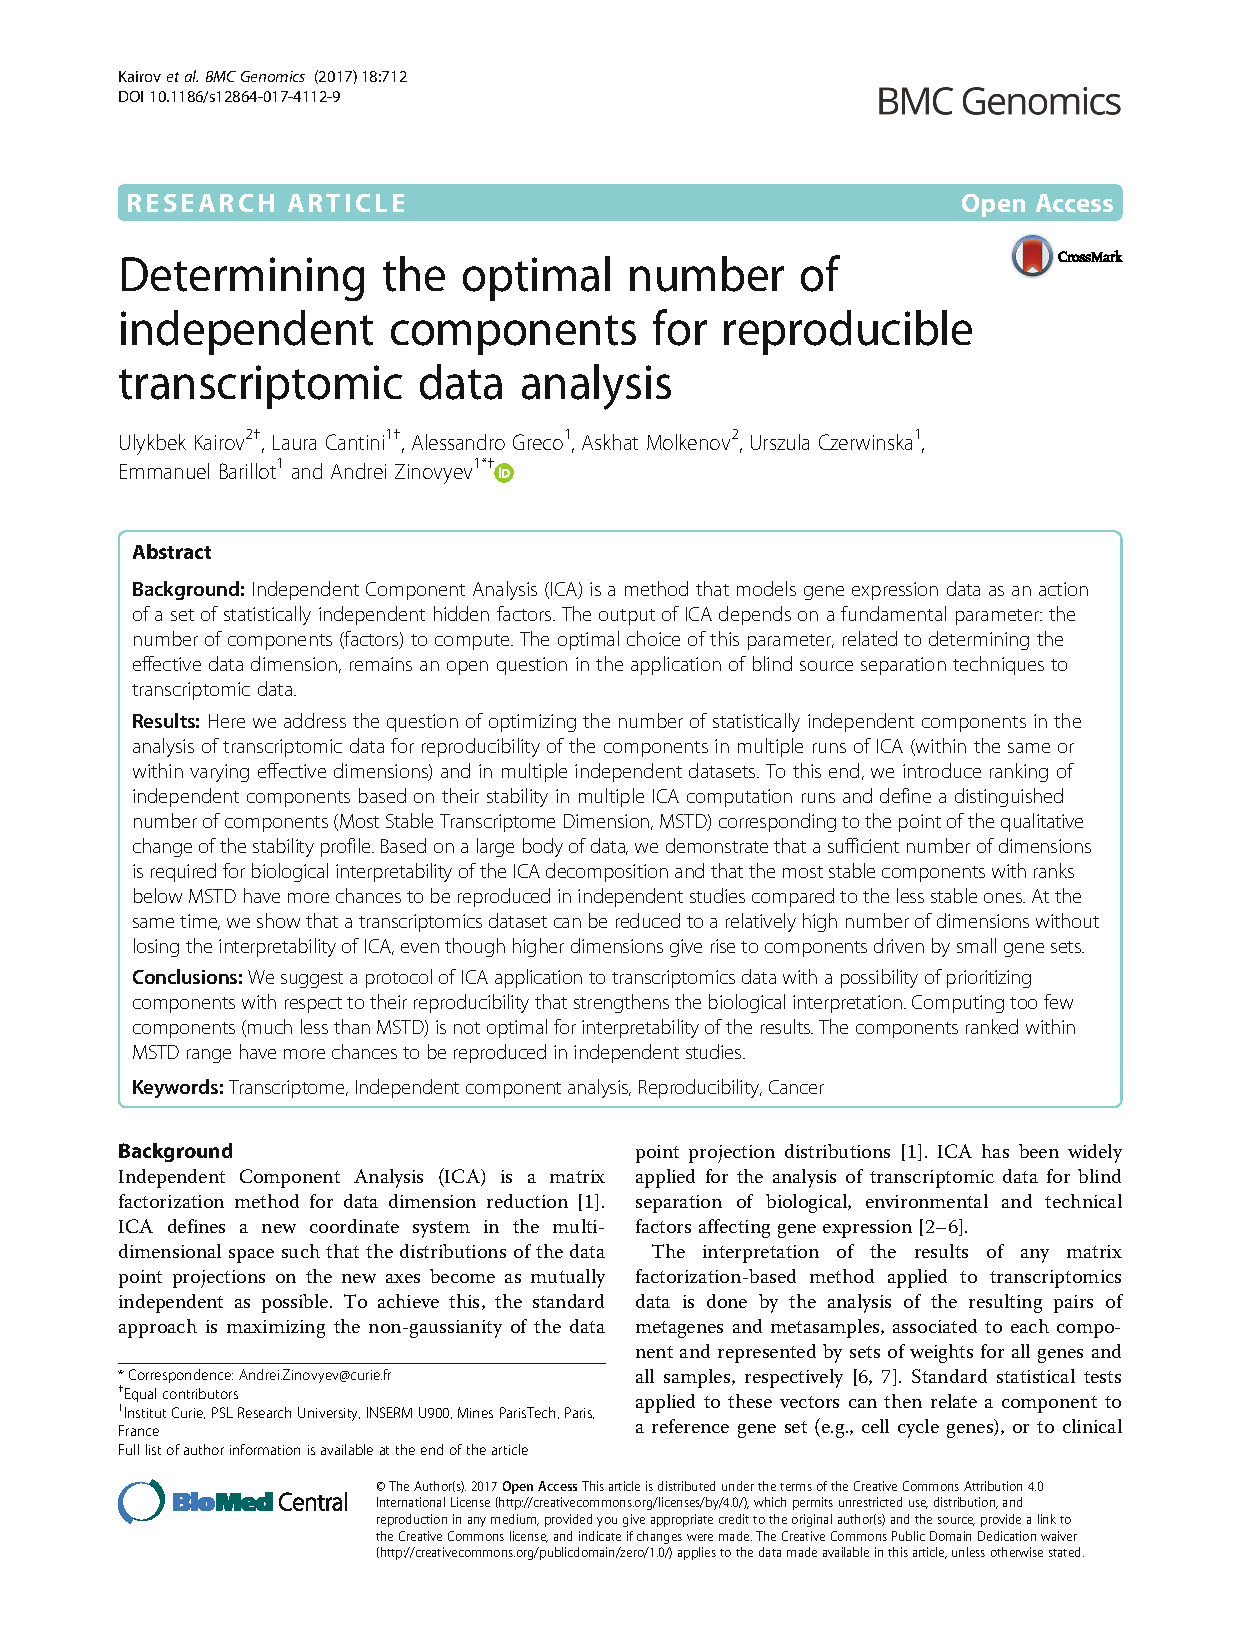
\includepdf[pages={1-}, scale=1]{pdf-ext/BMCMSTD.pdf}

\hypertarget{section-1}{%
\section{}\label{section-1}}

\hypertarget{reproducibility-of-nmf-versus-ica-vs-cam}{%
\section{REPRODUCIBILITY OF NMF VERSUS ICA (VS
CAM?)}\label{reproducibility-of-nmf-versus-ica-vs-cam}}

NMF and ICA are both algorithms often applied to solve blind source
deconvolution problem. NMF gained a popularity as a tool of
transcriptomic analysis mainly thanks to the publications
{[}publicaition\_list{]}. However, the non-negativity contraint, an
attractive concept in the case of non-negative transcriptome counts, may
be a reason why the reusults of NMF decomposition are not the best
candidate for our deconvolution task. We observed that NMF-based
metagenes are less reprouctible between different transcriptomic
datasets than ICA-based metagenes.

\hypertarget{comparing-metagenes-obtained-with-nmf-vs-ica.}{%
\subsection{Comparing metagenes obtained with NMF vs
ICA.}\label{comparing-metagenes-obtained-with-nmf-vs-ica.}}

We compared the reproducibility of NMF and ICA through decomposition of
four breast cancer datasets (BRCATCGA, METABRIC, BEK, WAN){[}ref{]}.
Those datasets were selected because of their size (number of samples
\textgreater{} 50) and because they were available in not centred format
necessary for NMF.

For NMF the procedure was following:

\begin{itemize}
\tightlist
\item
  data was transformed into log2
\item
  zero rows were removed
\item
  the algorithm assesing cophentic index was applied to chose optimal
  number of components
\item
  datasets were decomposed with matlab NMF implementation from Brunet et
  al. \citep{Brunet} into (i) number of components suggested by
  cophenetic coefficient (ii) MSTD dimension (iii) 50 components
  (approaching overdecomposition)
\item
  the obtained metagenes were decorellated from the mean using a linear
  regression model
\end{itemize}

For ICA, the procedure was following:

\begin{itemize}
\tightlist
\item
  data were transformed into log2
\item
  transformed data were mean-centered by gene
\item
  our implementation of MSTD (most stable transcriptomic dimension) from
  \citep{Ulykbek2017} was used to evaluate most stable dimension
\item
  datasets were demposed into (i) MSTD dimension and (ii) 50 components
  (approaching overdecomposition) with matlab implementantion of fastICA
  with icasso stabilisation
\end{itemize}

We did not decompose ICA into low number of components as we consider it
as strong underdecomposition and we suspect signals would not be the
most reproducible. We limited the over decomposition higher than 50 with
NMF as for our biggest dataset (METABRIC) NMF decomposition into 50 took
30245 minutes (3 weeks).

Then separately for NMF and ICA, we correlated all obtained metagens
with each other and with known Biton et al.~metagenes (obtain from
previous ICA decompostion applied pan-cancer). We represented the
results in a form of a correlation graph where nodes are metagenes from
different datasets and decompostion levels and edge width corresponds
peasron correaltion coefficients (Fig \ref{fig:ICAvsNMF}).

\begin{figure}

{\centering 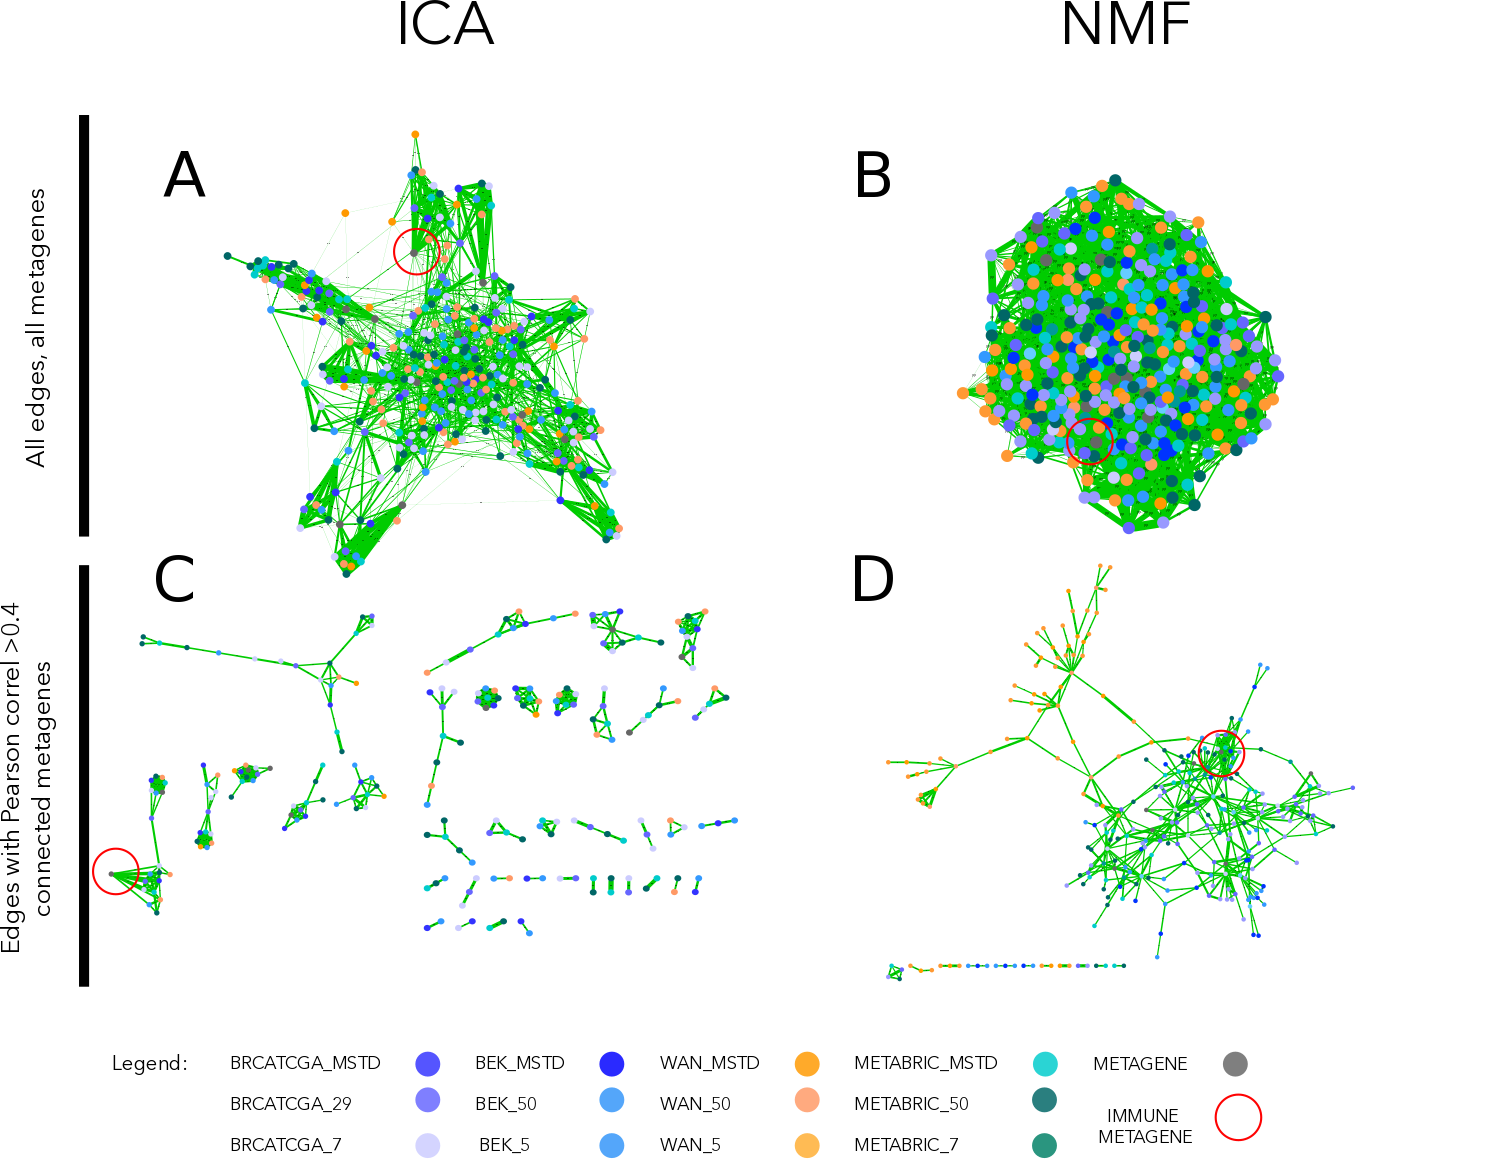
\includegraphics[width=1\linewidth]{figures-ext/ICANMF} 

}

\caption{\textbf{Correlation graph of ICA and NMF multiple
decompositions.} In the upper part of the figure (A,B) we observe the
correlation graph of all metagenes (ICA or NMF-based) disposed using
edge-weighted bio layout. In the lower part of the figure (C,D) we
applied \textgreater{}0.4 thereshold in order to filter the edges. In
the case of ICA (C), remaining nodes form pseudo-cliques, immune-related
pseudo-clique is highlighted. In the case of NMF (D), components cluster
by dataset. Edges' width coressponds to Pearson correlation coefficient.
Node colors correspond to dataset from which a metagene was obtained
(see legend).}\label{fig:ICAvsNMF}
\end{figure}












We hoped to observe a subset of components from different datasets (no
matter the decomposition level) correlate with each strongly and much
less with other components in order to confirm that the signal is
reproducible (can be found in several dataset) and specific. We used the
Biton et al.~componets here to help with eventual identification of
signals (labelling). What we observe from ICA-decomposition that indeed,
without applying any threshold some emerging clusters can be remarked
and after application of \textgreater{}0.4 threshold on the correlation
coeffcient pseudo-cliques emerge. While metagenes from NMF-decpmpostion
are more tighlty connected globally and when the threshold is applied,
remaing metagenes do not form clear clusters but group by data set. In
NMF decomposition if it hard to define different signals as the datasets
seem to be all related to each other. We can see from (Fig
\ref{fig:ICAvsNMF}D) that the IMMUNE signal is correlated
\textgreater{}0.4 with a high number of NMF components that are also
linked to some other components. In ICA (Fig \ref{fig:ICAvsNMF}C)
components related to the IMMUNE metagens form a pseudo-clique that is
related with one link to INTERFERON metagene.

This simple analysis illustrates that NMF applied to cancer
transcriptomes decomposes them to metagenes that are not highly
reproductible between datasets. In practice, it will not always be
possible to work with big cohorts and the same processing methods. Using
ICA for decomposition gives mor credit that it will be possible to use
the obtained metagenes as reference in which new data of similar type
could be projected.

\emph{to do:}

\begin{itemize}
\item
  \emph{quantify: with clustering coefficient?}

  ​
\item
  Explain why ICA is more reproducible
\end{itemize}

\hypertarget{impact-of-modification-of-signatures-list-on-result-for-signature-based-deconvolution-methods}{%
\section{Impact of modification of signatures list on result for
signature-based deconvolution
methods}\label{impact-of-modification-of-signatures-list-on-result-for-signature-based-deconvolution-methods}}

Carry on a ``sensitivity study'':

\begin{itemize}
\tightlist
\item
  remove some \% of genes from basis matrix or marker gene list
\item
  evaluate how it changes results
\end{itemize}

\hypertarget{deconica}{%
\chapter{Deconvolution of transcriptomes and
methylomes}\label{deconica}}

We describe our methods in this chapter. The pre-eliminary pipeline and
simple results are described in the manuscript submitted to
Springer-Verlag's Lecture Notes in Computer Science
(\href{http://www.springer.com/gb/computer-science/lncs}{LNCS}) entitled
\textbf{Application of Independent Component Analysis to Tumor
Transcriptomes Reveals Specific And Reproducible Immune-related Signals}
that is placed at the end of this chapter. In the final thesis final
pipeline will be split into following structure

\hypertarget{from-blind-deconvolution-to-cell-type-quantification-general-overview}{%
\section{From blind deconvolution to cell-type quantification: general
overview}\label{from-blind-deconvolution-to-cell-type-quantification-general-overview}}

Few lines describing our idea

Figure?

\hypertarget{the-ica-based-deconvolution-of-transcriptomes}{%
\subsection{The ICA-based deconvolution of
Transcriptomes}\label{the-ica-based-deconvolution-of-transcriptomes}}

\begin{itemize}
\tightlist
\item
  remind shortly ICA
\item
  describe stabilisation procedure \emph{icasso}
\item
  explain IC-metagene concept
\end{itemize}

If completed add related section about two other ways of getting
metagenes

\begin{itemize}
\tightlist
\item
  attractor metagenes
\item
  k-lines
\end{itemize}

\hypertarget{interpretation-of-independent-components}{%
\subsection{Interpretation of Independent
components}\label{interpretation-of-independent-components}}

\hypertarget{correlation-based-identification-of-confounding-factors}{%
\subsubsection{Correlation based identification of confounding
factors}\label{correlation-based-identification-of-confounding-factors}}

\hypertarget{identification-of-immune-cell-types-with-enrichment-test-other}{%
\subsubsection{Identification of immune cell types with enrichment test
/
other}\label{identification-of-immune-cell-types-with-enrichment-test-other}}

\hypertarget{transforming-metagenes-into-signature-matrix}{%
\subsection{Transforming metagenes into signature
matrix}\label{transforming-metagenes-into-signature-matrix}}

\hypertarget{regression-based-estimation-of-cell-type-proportions-solving-system-of-equations}{%
\subsection{Regression-based estimation of cell-type proportions :
solving system of
equations}\label{regression-based-estimation-of-cell-type-proportions-solving-system-of-equations}}

\hypertarget{deconica-r-package-for-ica-based-deconvolution}{%
\section{\texorpdfstring{\emph{DeconICA} R package for ICA-based
deconvolution}{DeconICA R package for ICA-based deconvolution}}\label{deconica-r-package-for-ica-based-deconvolution}}

This part of the chapter will be adapted from package vignettes

It will contain

\begin{itemize}
\item
  technical package description
\item
  user guide
\item
  examples
\end{itemize}

\hypertarget{demo}{%
\subsection{\texorpdfstring{\emph{Demo}}{Demo}}\label{demo}}

The package needs to installed and then imported.

\begin{Shaded}
\begin{Highlighting}[]
\CommentTok{#import package}
\KeywordTok{library}\NormalTok{(deconica)}
\end{Highlighting}
\end{Shaded}

Then we can perform our pipeline on sample data available in the package

\begin{Shaded}
\begin{Highlighting}[]
\CommentTok{#import sample data}
\KeywordTok{data}\NormalTok{(BRCA)}
\CommentTok{#decompose data}
\NormalTok{fastica.res <-}\StringTok{ }\KeywordTok{run_fastica}\NormalTok{ (}
\NormalTok{  BRCA,}
  \DataTypeTok{optimal =} \OtherTok{TRUE}\NormalTok{,}
  \DataTypeTok{row.center =} \OtherTok{TRUE}\NormalTok{,}
  \DataTypeTok{with.names =} \OtherTok{TRUE}\NormalTok{,}
  \DataTypeTok{gene.names =} \OtherTok{NULL}\NormalTok{,}
  \DataTypeTok{alg.typ =} \StringTok{"parallel"}\NormalTok{,}
  \DataTypeTok{method =} \StringTok{"C"}\NormalTok{,}
  \DataTypeTok{n.comp =} \DecValTok{100}\NormalTok{,}
  \DataTypeTok{isLog =} \OtherTok{TRUE}\NormalTok{,}
  \DataTypeTok{R =} \OtherTok{TRUE}
\NormalTok{)}
\CommentTok{#correlate obtained metagenes with Biton et al. }
\CommentTok{#metagenes (by default)}
\NormalTok{correlate.res <-}
\StringTok{  }\KeywordTok{correlate_metagenes}\NormalTok{(fastica.res}\OperatorTok{$}\NormalTok{S, fastica.res}\OperatorTok{$}\NormalTok{names)}
\CommentTok{#assign reciprocal components}
\NormalTok{assign.res <-}\StringTok{ }\KeywordTok{assign_metagenes}\NormalTok{(correlate.res}\OperatorTok{$}\NormalTok{r)}
\CommentTok{#identify components that are >0.1 correlated with }
\CommentTok{#immune and are not assigned to any other component}
\NormalTok{identify.immune <-}
\StringTok{  }\KeywordTok{identify_immune_ic}\NormalTok{(correlate.res}\OperatorTok{$}\NormalTok{r[, }\StringTok{"M8_IMMUNE"}\NormalTok{], assign.res[, }\DecValTok{2}\NormalTok{])}
\CommentTok{#test enrichment with fisher test in }
\CommentTok{#Immgen signatures (by default)}
\NormalTok{enrichment.res <-}\StringTok{ }\KeywordTok{gene.enrichment.test}\NormalTok{(}
\NormalTok{  fastica.res}\OperatorTok{$}\NormalTok{S,}
\NormalTok{  fastica.res}\OperatorTok{$}\NormalTok{names,}
  \KeywordTok{names}\NormalTok{(identify.immune),}
  \DataTypeTok{gmt =}\NormalTok{ ImmgenHUGO,}
  \DataTypeTok{alternative =} \StringTok{"greater"}\NormalTok{,}
  \DataTypeTok{p.adjust.method =} \StringTok{"BH"}\NormalTok{,}
  \DataTypeTok{p.value.threshold =} \FloatTok{0.05}
\NormalTok{)}
\end{Highlighting}
\end{Shaded}

The present state of the package is described in Fig
\ref{fig:deconICAflow}.

\begin{figure}

{\centering 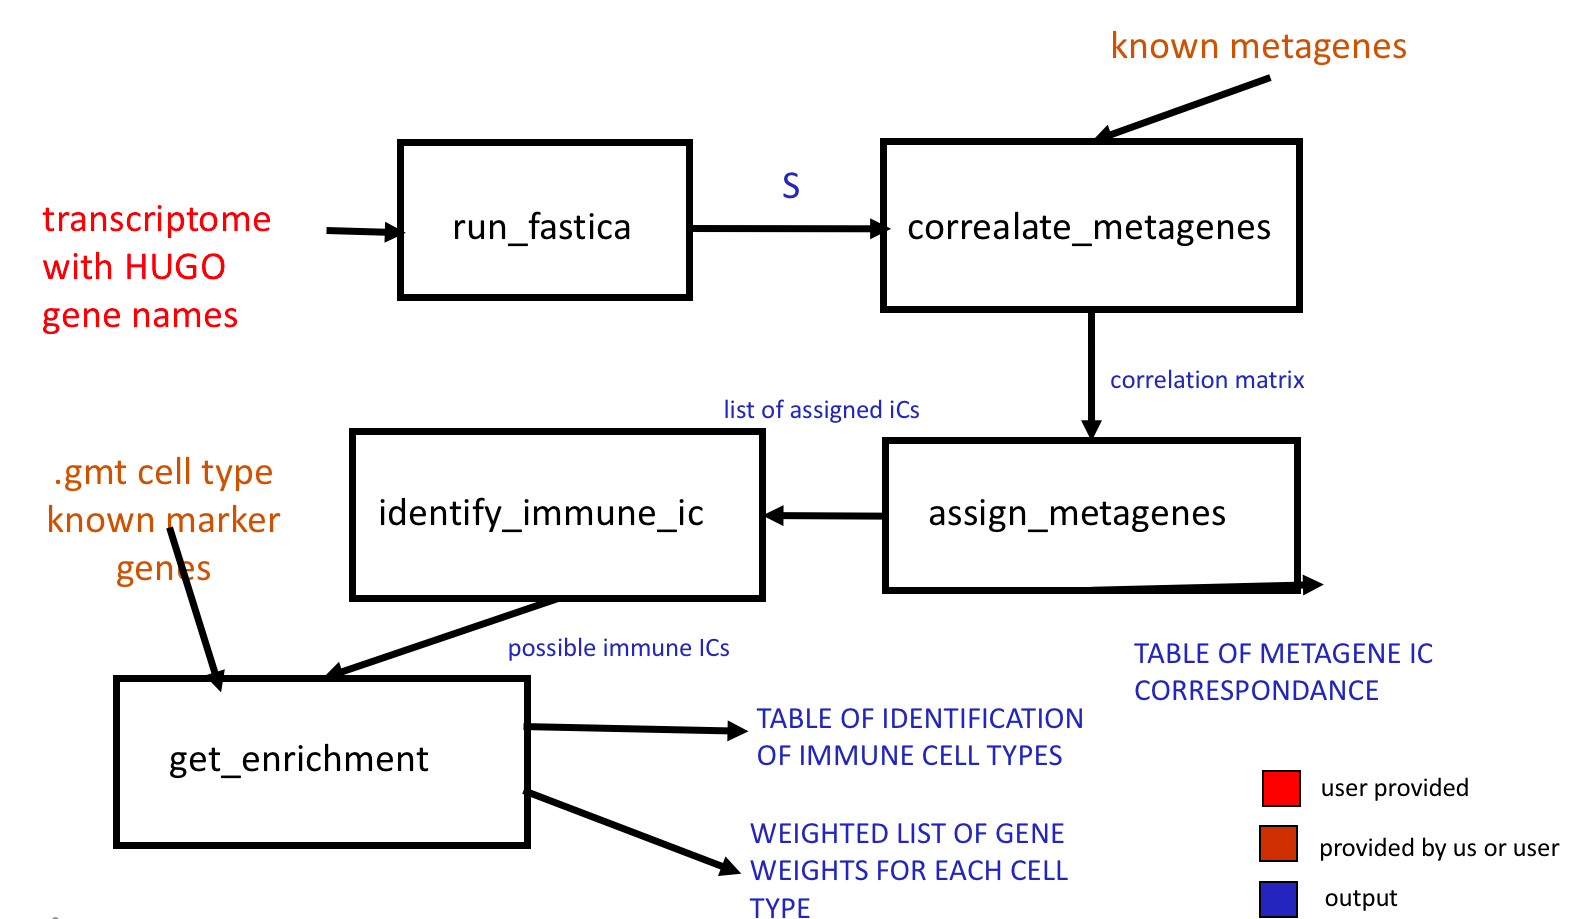
\includegraphics[width=1\linewidth]{figures-ext/deconICApipeline} 

}

\caption{\textbf{State of the deconICA package in
January 2018.} The flow chart illustrates existing functions in the R
package \emph{DeconICA}. Squares represent functions, red are
user-provided inputs, brown are inputs we provide but that can be
replaced easily by user and in blu we marked outputs.}\label{fig:deconICAflow}
\end{figure}







Next step will be:

\begin{itemize}
\tightlist
\item
  adding the metagenes selection and transformation into basis matrix
  for deconvolution
\item
  identifying confounding factors
\item
  estimating purity with an existing tool
\item
  running an equations solver (based on least squares or other type of
  regression) including basis matrix, confounding factors, purity
\item
  including regularisation factos
\item
  adding graphics
\item
  adding user interface
\item
  writing a demo (best interactive)
\end{itemize}

\newpage

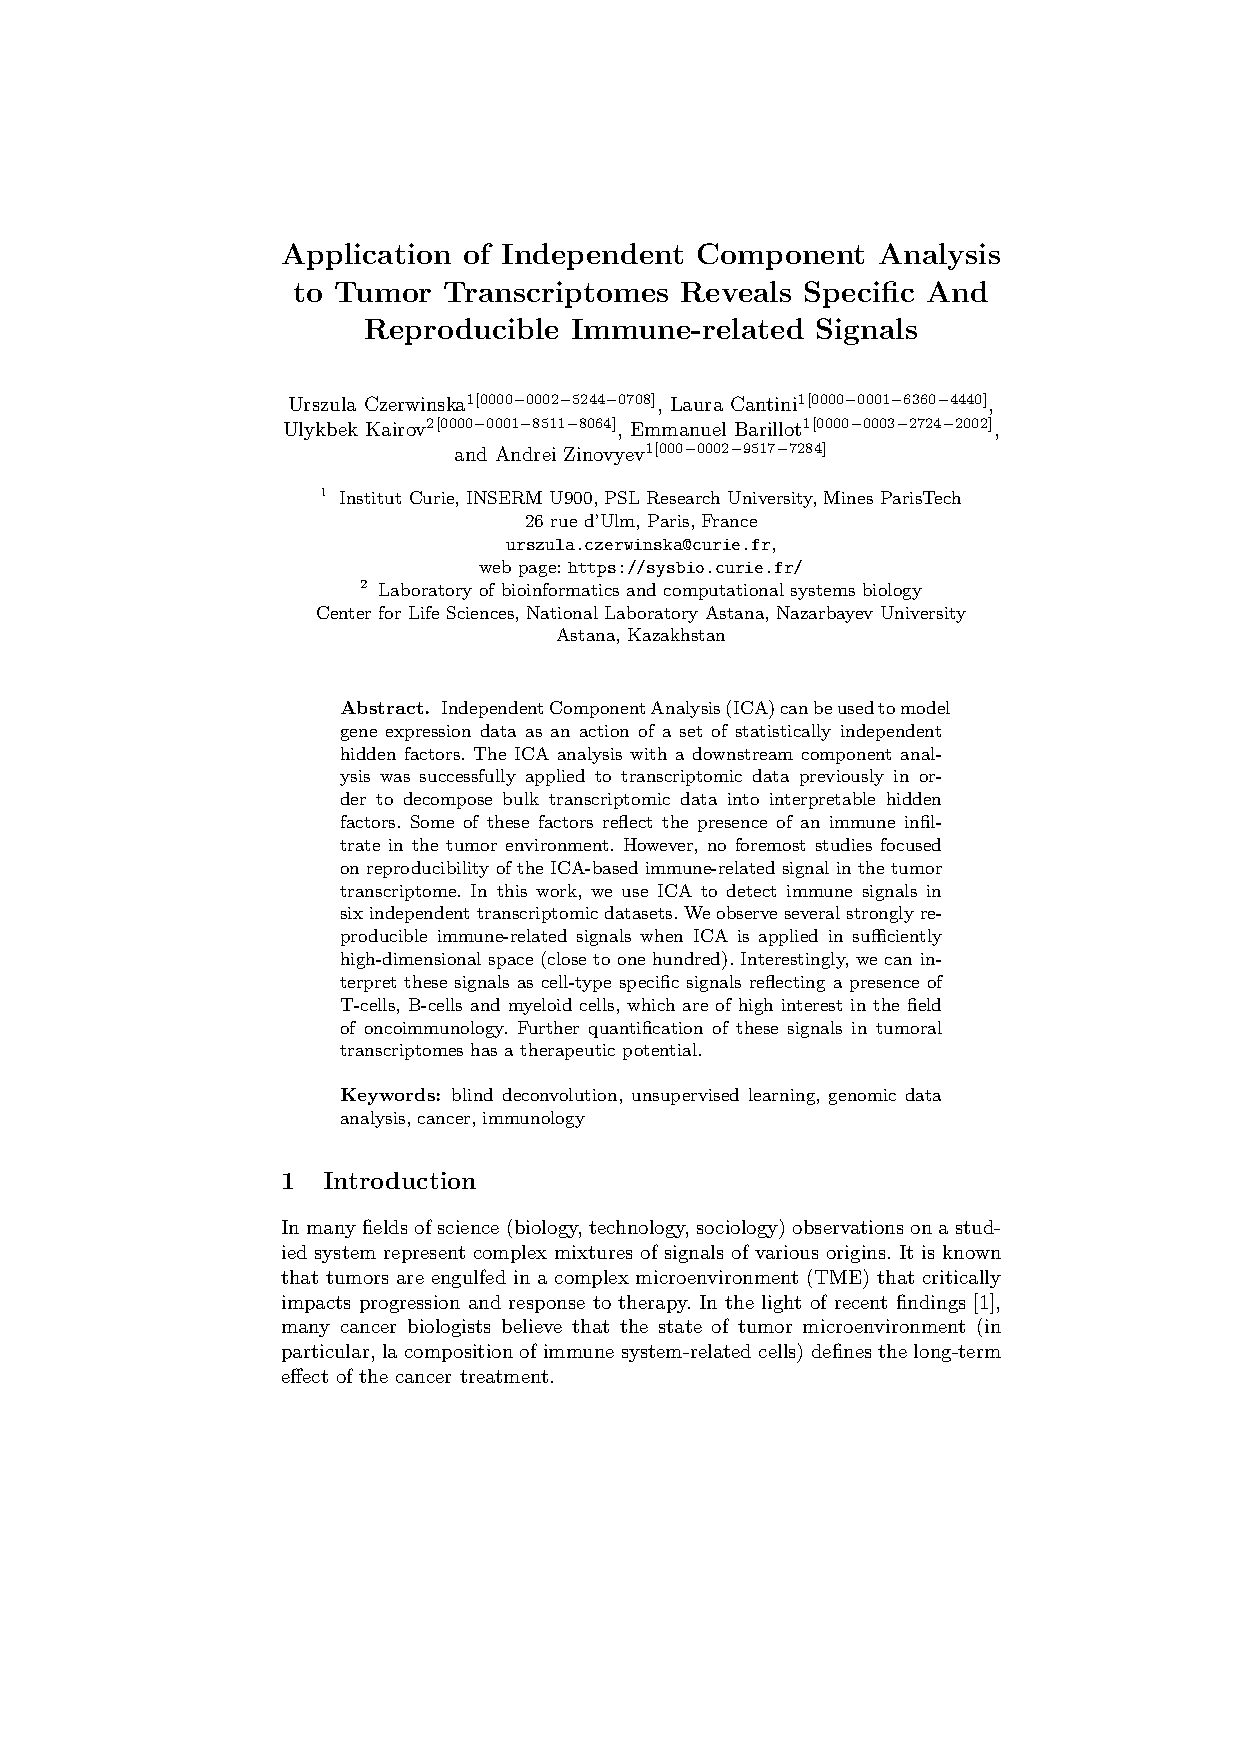
\includepdf[pages={1-}, scale=1]{pdf-ext/LVAICA.pdf}

\hypertarget{results}{%
\chapter{Comparative analysis of cancer immune
infiltration}\label{results}}

This chapter will include biological interpretation of Pan-cancer
analysis with DeconICA

\begin{itemize}
\item
  application to Breast cancer

  \begin{itemize}
  \item
    compare metagenes of the same cell type in different datasets
  \item
    compare metagenes of the same cell type in the same dataset (happens
    sometimes)
  \item
    compare A matrix (sample weights) with clinical metadata
  \item
    compare patients with opposite extreme phenotypes (the gene
    expression) with DEG ou others
  \item
    run enrichment with more specific list of genes ex. Th1/2/17 cells
    in T cels etc.

    ​
  \end{itemize}
\item
  application pan cancer

  \begin{itemize}
  \tightlist
  \item
    derivation of meta-metagenes for immune cell types
  \item
    above points are true for pan cancer
  \end{itemize}
\item
  follow up of Biton paper ?

  \begin{itemize}
  \tightlist
  \item
    \emph{Idea of Vassili from the lab meeting}, personally I am not
    sure if there is no conflict of interest with other members of the
    team
  \end{itemize}
\end{itemize}

\hypertarget{map}{%
\chapter{Heterogeneity of immune cell types}\label{map}}

We include here an extract of a \emph{ready to submit} article of
Kondratova et al. \textbf{(co-first authored by Urszula Czerwinska)} -
the abstract and figures which are result of work on single cell
heterogeneity.

Explication how deconvolution methodology can be used for analysis of
heterogeneity of immune cells

\begin{itemize}
\item
  describe the context briefly
\item
  describe more in details my part - data analysis of single cell data
\end{itemize}

To be defined:

\begin{itemize}
\tightlist
\item
  add CAFS (that will maybe appear in \emph{JBM})
\item
  add unpublished analysis made for the Nature Immunology \emph{Michea
  et al.} paper (to be defined)
\item
  The single T-cell study (if done)
\end{itemize}

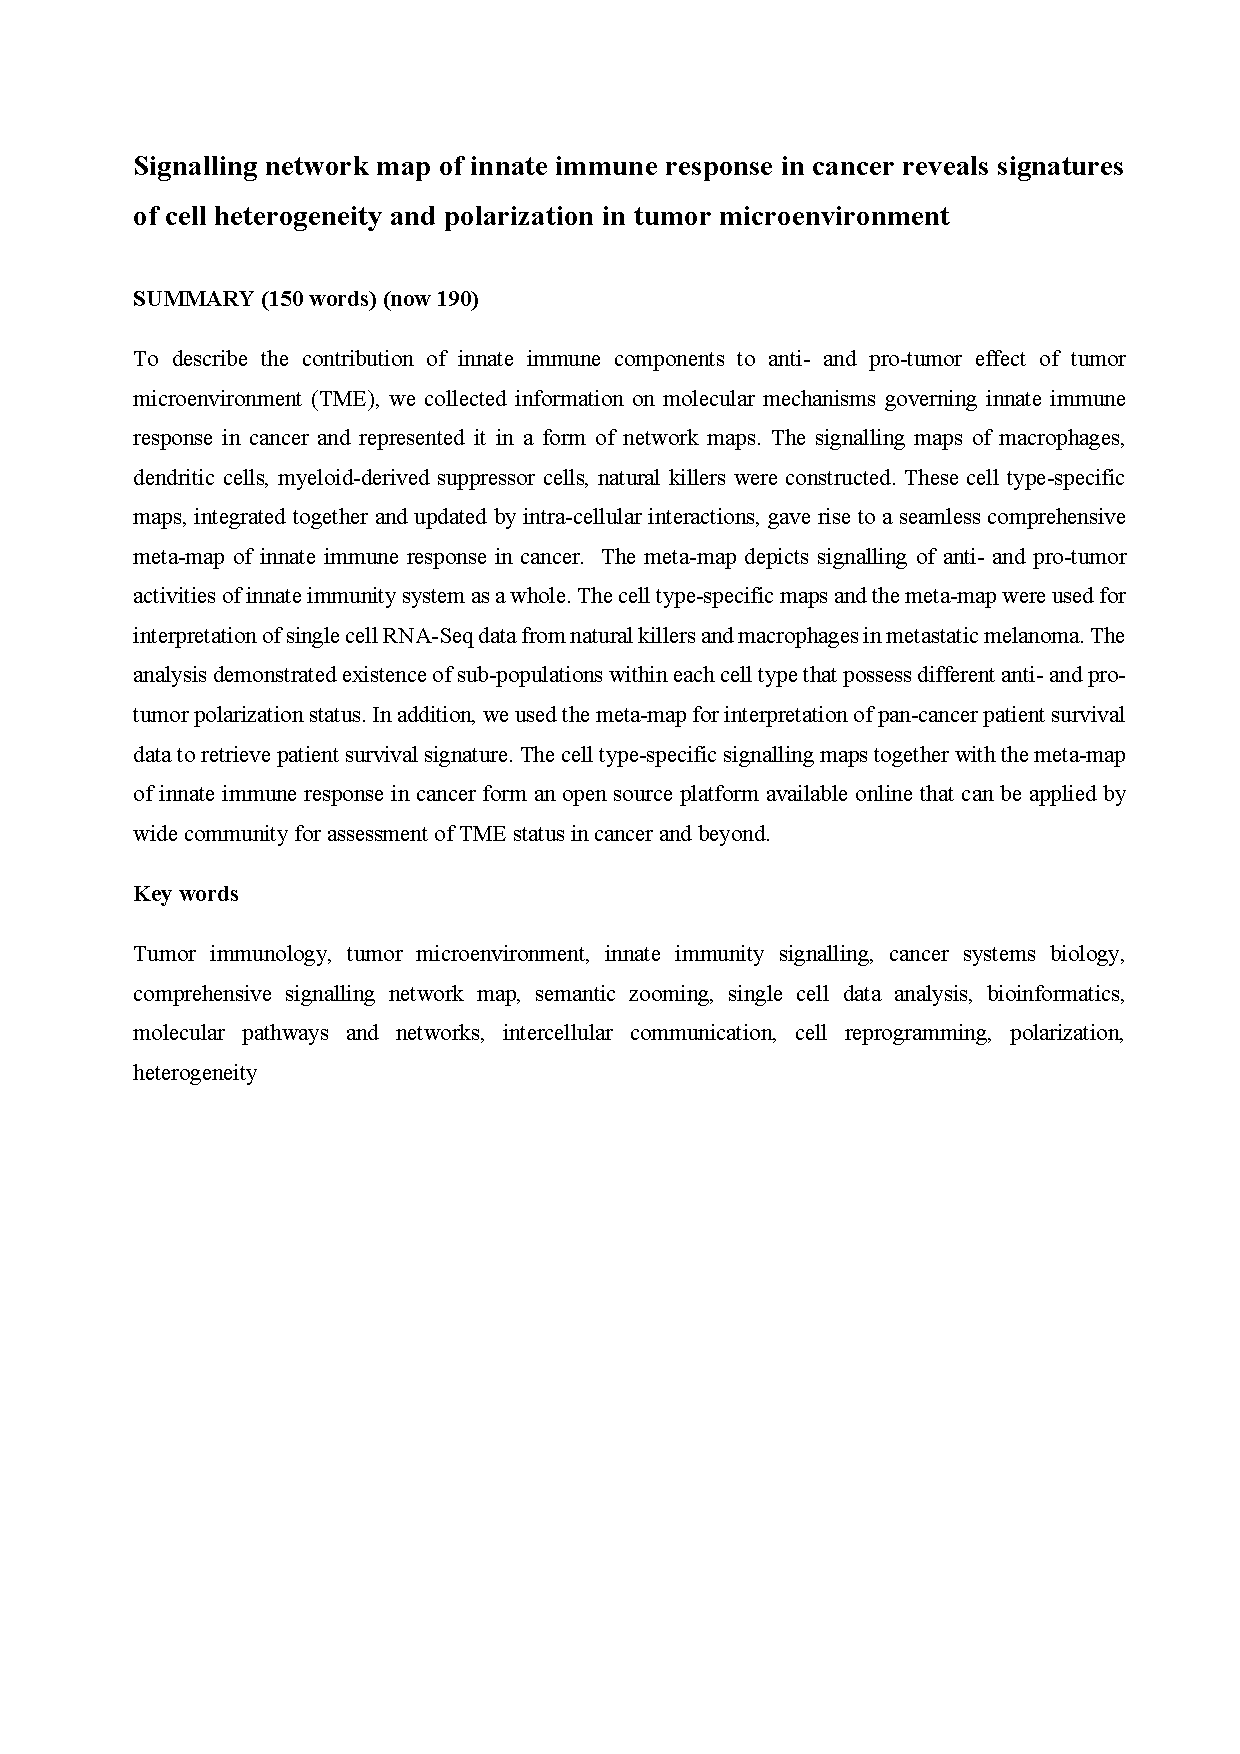
\includepdf[pages={1-}, scale=1]{pdf-ext/ImmuneMap.pdf}

\hypertarget{part-discussion}{%
\part{Discussion}\label{part-discussion}}

\hypertarget{discussion}{%
\chapter{Discussion}\label{discussion}}

\hypertarget{conclusions}{%
\chapter{Conclusions and perspectives}\label{conclusions}}

Here we will have some interesting and well-written conclusion that will
validate the quality of this thesis.

Problems:

\begin{itemize}
\item
  reproducibility of other tools (code accessing, making work,
  pre-processing)
\item
  no-spatial dimension
\item
  heterogeneity - analyse sample by samples (need of big dimension)
\item
  time dimention
\item
  validation - no gold statndard
\item
  our solution - more contex specific but less interpretable?
\end{itemize}

A major part of this thesis has been to reproduce earlier
work{[}7{]}{[}8{]}, and it has been time consuming to try to reproduce
different approaches or scripts. It has been brought up that other
scientists have struggled - and many failed - to reproduce another
scientists work{[}48{]}. The article states that of 1,576 researchers,
over 70\% have failed to reproduce others work and over 50\% have failed
to reproduce their own. 52\% of the participants in the survey state
that is is a ``significant crisis'', which indicates that we could call
this a ``reproducibility crisis''{[}48{]}. Such high numbers may suggest
in- accurate or poor documentation of the different steps towards
achieving the results, or even going as far as suggesting untrustworthy
results. The latter is a bold statement, but according to the article,
less than 31\% believe that struggles to reproduce published results are
due to wrong results{[}48{]}.

Moreover, the immune cells can be situated in different locations,
either in the core, in the invasive margin or in the adjacent tertiary
lymphoid structures (TLS), ectopic lymphoid formations found in
inflamed, infected, or tumoral tissues exhibiting all the
characteristics of structures in the lymph nodes (LN) associated with
the generation of an adaptive immune response (Dieu-Nosjean et
al.~2014): a correlation has been found between high densities of TLS
and prolonged patient's survival in more than 10 different types of
cancer (Sautès-Fridman et al.~2016).

For instance, CD8+ T cells can be visible in both the invasive margin
and the core of the tumor, while the TLS seem to lack these cells. In
addition, the mixture of immune cells can vary differently in relation
to tumor types. Some components of the immune contexture, more than
others, are helpful in terms of good prognosis: this fact is shared by
multiple papers, such as Dave et al.~2004, which paved the way in the
early years of the XXI century, while in Parker et al.~2008 and Parker
et al.~2009

----

. In the case of T cells and cancer, although the total frequencies of
tumor-specific T cells are difficult to assess (due to uncertainties
about the range of targets, see below), reports of blood-derived
tumor-specific T cells suggest that these frequencies are low (much less
than 1\% of CD8þ T cells, which typically make up 10\%--20\% of
peripheral blood mononuclear cells; refs. 50, 51). Therefore, at least
in the case of blood, a large part of the signal measured in bulk T-cell
profiles should originate from irrelevant cells. In tumor tissues, the
problem is certainly less severe, in that tumor-infiltrating T cells are
likely enriched for tumor-specific T cells. However, as discussed above,
because the immunologic composition of tumor tissues is complex and
heterogeneous, similar efforts dedicated to identifying, quantifying,
and profiling relevant (tumor-specific) T cells are still needed.

\hypertarget{annexes}{%
\chapter*{Annexes}\label{annexes}}
\addcontentsline{toc}{chapter}{Annexes}

\hypertarget{dc-subtypes}{%
\section*{Dc subtypes}\label{dc-subtypes}}
\addcontentsline{toc}{section}{Dc subtypes}

\hypertarget{dreamidea-challenge}{%
\section*{DreamIdea Challenge}\label{dreamidea-challenge}}
\addcontentsline{toc}{section}{DreamIdea Challenge}

\hypertarget{full-list-of-publications}{%
\section*{Full list of publications}\label{full-list-of-publications}}
\addcontentsline{toc}{section}{Full list of publications}

\hypertarget{cv}{%
\section*{CV}\label{cv}}
\addcontentsline{toc}{section}{CV}

\newpage

\hypertarget{post-scriptum-thesis-writing}{%
\chapter*{Post Scriptum: Thesis
writing}\label{post-scriptum-thesis-writing}}
\addcontentsline{toc}{chapter}{Post Scriptum: Thesis writing}

This Thesis is written in
\href{https://github.com/rstudio/bookdown}{\emph{bookdown}}. I have
chosen this form as it can easily compile to \emph{LaTeX}, PDF, MS Word,
ebook and html. Optimally, the final manuscript will be also published
online in a form of an open source
\href{https://www.gitbook.com/about}{gitBook} and an ebook including
interactive figures and maybe even data demos. Another good reason for
using \href{https://github.com/rstudio/bookdown}{\emph{bookdown}} is its
simple syntax of markdown and natural integration of code snippets with
.Rmd. It reduces formatting time and give multiple outputs.

The template of for this thesis manuscript was adapted from \emph{LaTeX}
template provided by University Paris Descartes.

Citations are stocked in Mendeley Desktop and exported to .bib files
automatically.

\addcontentsline{toc}{chapter}{Bibliography}

\bibliography{00-Inter,01-Intro02,02-MathIntro,packages,UCzcite}


\end{document}
